\documentclass[11pt]{article}
\usepackage[utf8]{inputenc}
\usepackage[T1]{fontenc}
\usepackage{lmodern}
\usepackage[margin=1in]{geometry}
\usepackage{amsmath,amssymb,amsthm,mathtools}
\usepackage{bm}
\usepackage{textcomp}
\usepackage{graphicx}
\usepackage{booktabs}
\usepackage{multirow}
\usepackage{threeparttable}
\usepackage{siunitx}
\sisetup{group-separator={,},group-minimum-digits=4,detect-all}
\usepackage{xcolor}
\usepackage[font=small,labelfont=bf]{caption}
\usepackage{subcaption}
\usepackage[numbers,sort&compress]{natbib}
\usepackage{microtype}
\usepackage[colorlinks=true,linkcolor=blue!50!black,citecolor=blue!50!black,urlcolor=blue!50!black]{hyperref}
\usepackage[capitalise,noabbrev]{cleveref}

\newtheorem{proposition}{Proposition}
\newtheorem{lemma}{Lemma}
\newtheorem{corollary}{Corollary}
\theoremstyle{definition}
\newtheorem{definition}{Definition}
\theoremstyle{remark}
\newtheorem{remark}{Remark}

% Shared notation. Use these macros in every section.
\newcommand{\E}{\mathbb{E}}
\newcommand{\Prob}{\mathbb{P}}
\newcommand{\Var}{\operatorname{Var}}
\newcommand{\Cov}{\operatorname{Cov}}
\newcommand{\Corr}{\operatorname{Corr}}
\newcommand{\sgn}{\operatorname{sgn}}
\newcommand{\ind}[1]{\mathbf{1}\{#1\}}
\newcommand{\dd}{\mathrm{d}}
\newcommand{\F}{\mathcal{F}}
\newcommand{\N}{\mathcal{N}}
% model objects
\newcommand{\pr}{p}                 % fair price / probability, p_t
\newcommand{\Zt}{Z}                 % probit price, Z_t = \Phi^{-1}(p_t)
\newcommand{\tauexp}{\tau}          % time to the scheduled end of information
\newcommand{\Vrem}{V}               % remaining information variance V_t
\newcommand{\irate}{\lambda}        % information rate lambda_t = s_t^2 / V_t
\newcommand{\ustd}{u}               % standardised innovation
\newcommand{\Fmed}{F}               % implied median of a ladder
\newcommand{\satm}{\sigma_{\mathrm{ATM}}}
\newcommand{\hbarimp}{\bar h}       % implied average hazard
\newcommand{\cents}{\,\text{\textcent}}
\newcommand{\estim}{estimation sample}


\title{Black--Scholes for Binaries: Information Clocks, Jumps and Smiles\\in Prediction-Market Prices}
\author{[Author names]\\[2pt]\small [Affiliation]}
\date{November 2026}

\begin{document}
\maketitle
\begin{abstract}
The fair price of a binary event contract is a bounded martingale that ends at zero or one, so
its total variance is fixed by its initial price. We develop an option-pricing framework for such
contracts.

In the base model, the contract is a Bachelier digital option on a latent Gaussian score. Its price
solves the Black--Scholes equation with a digital payoff and has an exact transition law. The role
of implied volatility is played by an \emph{information clock}: the rate at which remaining
uncertainty is resolved. We extend the model with SABR-type stochastic volatility, a general
backbone and jumps, and adapt it to strike ladders, which are strips of digitals with an implied
smile, and to deadline contracts, which are reduced-form hazard claims.

Calibrating on Kalshi, out of sample, we use hourly quotes on 47,500 contracts, 24,000 ladder
snapshots, 5,900 deadline contracts and full order-book recordings of in-game sports markets.
Prices respect the variance budget, and the clock is category-specific: uniform within games, as in
Stern's Brownian model; back-loaded for weather; nearly flat before games; and rising steeply into
deadlines.

Half or more of the variance arrives in jumps, even at the scale of seconds. Volatility scales with
the price close to the Wright--Fisher backbone, and it is stochastic with half-lives of 7--21
hours. Ladder smiles are convex and sticky in moneyness.

Implied tail mass, implied hazards and implied variance all exceed their realized counterparts: a
tail-and-time form of the favourite--longshot bias, bounded by the one-cent tick and fees.

\end{abstract}

\section{Introduction}\label{sec:intro}
Prediction markets have become a large, regulated asset class. In the United States, an exchange
such as Kalshi lists hundreds of thousands of binary contracts on sports, weather, entertainment,
politics and public statements, many of them each week. Their prices are routinely read as
probabilities \citep{wolferszitzewitz2004,wolferszitzewitz2006}. A large literature asks whether
those probabilities are calibrated, documenting in particular the favourite--longshot bias
\citep{griffith1949,thalerziemba1988,snowbergwolfers2010,burgi2025}.

Much less is known about how these prices \emph{move}. Option pricing begins from a model of the
dynamics; the analogue for an event contract is largely missing. Such a model is needed to price
derivatives of prediction-market prices, to manage the risk of quoting them, to read a probability
correctly when it has just jumped, and to say what ``volatility'' even means for a security that
must end at 0 or 1.

This paper develops such a model and calibrates it on Kalshi. The starting point is simple: the
fair price of a binary contract is a bounded martingale that terminates at 0 or 1. Its total
variance over its life is therefore fixed at $\pr_0(1-\pr_0)$ (\cref{lem:variance}). What a model
must describe is \emph{when}, \emph{at which price levels} and \emph{in what shape} this fixed
variance is released.

We formalise this with a latent Gaussian score. The contract pays if the score ends above zero, so
the price is a Bachelier digital option. It solves the Black--Scholes equation with a digital payoff
and has an exact transition law (\cref{prop:m0}). The role of implied volatility is taken by an
\emph{information clock}: the rate at which the remaining uncertainty is resolved. We then add a
SABR-type stochastic volatility with a general backbone (M1) and jumps (M2). We extend the framework
to two other contract structures that Kalshi lists at scale:
\begin{itemize}
  \item \emph{ladders} of contracts on one numeric outcome, such as a daily high temperature or a
  points total. These are strips of digital options with an implied distribution, an implied
  volatility per strike and a smile.
  \item \emph{deadline} contracts that pay if an event occurs by a date. These are reduced-form
  credit claims with an implied hazard term structure and a theta.
\end{itemize}

We calibrate the three branches on several data sets:
\begin{itemize}
  \item 4.8 million hourly quote observations on 47,500 single contracts;
  \item 24,000 snapshots of 10,200 ladders in 9,200 events;
  \item 26,000 priced observations of 5,900 deadline contracts;
  \item full order-book recordings of 50 in-game sports markets.
\end{itemize}
Parameters are chosen on data before October 2026 and evaluated on October.

Our findings can be summarised as seven stylized facts.
\begin{enumerate}
  \item \textbf{Prices are fair in level and in total variance.} The variance identity holds within
  a few percent in the broad categories.
  \item \textbf{Clocks differ sharply by contract type.} In-game sports follow Stern's Brownian game
  almost exactly, with a uniform clock. Weather information is back-loaded into the final hours.
  Pre-game sports learn almost nothing. Deadline contracts carry an implied hazard that rises
  steeply into the deadline.
  \item \textbf{Variance arrives in jumps.} Half or more of price variance comes from discrete moves,
  even within games at the scale of seconds. Prices drift toward resolution more slowly than the
  Gaussian model predicts. Outside sports the one-cent grid accounts for this; in sports, jumps do.
  \item \textbf{The backbone is close to Wright--Fisher.} Price volatility scales like
  $[\pr(1-\pr)]^\beta$ with $\beta$ between 0.3 and 0.8; the logit-normal model ($\beta=1$) is
  rejected everywhere.
  \item \textbf{Volatility is stochastic but short-lived,} with half-lives of 7--21 hours outside weather.
  \item \textbf{Ladders have a smile, and it moves with the market.} The smile is sticky in moneyness
  rather than in strike. Implied widths and skews are close to calibrated, but implied tails are
  too heavy.
  \item \textbf{Tails and time are overpriced.} Implied tail mass across strikes, implied hazards
  before deadlines and implied variance before games all exceed their realized counterparts.
  Prices of deadline contracts decay toward zero at only a third to two-thirds of the model rate.
\end{enumerate}
These premia are the favourite--longshot bias in its cross-sectional and term-structure forms. The
one-cent tick and fees bound them to a few cents per contract.

The paper proceeds as follows.
\begin{itemize}
  \item \Cref{sec:lit} reviews related work.
  \item \Cref{sec:data} describes the market and the data.
  \item \Cref{sec:model} develops the model.
  \item \Cref{sec:method} describes the estimators.
  \item \Cref{sec:results} reports the results.
  \item \Cref{sec:discussion} discusses their interpretation and limitations.
  \item \Cref{sec:conclusion} concludes.
\end{itemize}


\section{Related literature}\label{sec:lit}
This paper draws on four literatures: prediction-market prices as probabilities, models of
probability-price dynamics, option pricing and the volatility smile, and reduced-form credit
models.

\paragraph{Prediction-market prices as probabilities.} \citet{wolferszitzewitz2004} survey prediction
markets and their forecasting record. \citet{manski2006} and \citet{wolferszitzewitz2006} ask when
an equilibrium price equals a mean belief. \citet{berg2008} document long-run accuracy in the Iowa
Electronic Markets, and \citet{pageclemen2013} find that prediction markets are well calibrated
except for contracts with long horizons. In betting markets the dominant departure from
calibration is the favourite--longshot bias: longshots are overpriced relative to their win
frequency \citep{griffith1949,thalerziemba1988}. \citet{snowbergwolfers2010} attribute it to
misperception of small probabilities rather than risk love. \citet{ottaviani2008} survey the
explanations. On Kalshi, \citet{burgi2025} use transaction data on more than 300,000 contracts.
They document a favourite--longshot bias that is stronger for takers than for makers, and model it
as modest belief disagreement with an overestimation of small probabilities.
\citet{rothschildsethi2016} study trader types and microstructure in a political prediction market.

These papers study the \emph{level} of prices relative to outcomes. We study how prices
\emph{move}. We also show that the favourite--longshot bias reappears, in different guises, in the
cross-section of strikes and in the term structure of deadlines.

\paragraph{Dynamics of probability prices.} \citet{stern1994} models the score difference of a game
as a Brownian motion. The win probability is then a normal distribution function of the lead,
scaled by the square root of time remaining: our M0 with a uniform clock.
\citet{polsonstern2015} invert betting lines to obtain the implied volatility of a game, and
\citet{fengpolsonxu2016} extend the approach to soccer with a Skellam process.

\citet{archakipeirotis2009} derive the volatility of a binary contract's price from latent ability
diffusions. They show that volatility depends on the price and on time to expiration, and that the
structural model beats GARCH in forecasting InTrade volatility. \citet{taleb2018} uses the same
construction to argue that a well-calibrated election forecast must stay close to one half when
uncertainty is high.

Two recent papers are the closest to ours.
\begin{itemize}
  \item \citet{dalen2025} proposes a ``Black--Scholes for prediction markets''. It models log-odds as
  a jump-diffusion whose drift is fixed by the martingale condition. It describes an EM
  calibration that separates diffusion from jumps, and a layer of variance and correlation
  derivatives. Its validation is largely on synthetic paths.
  \item \citet{xi2026} estimate a structural volatility model on a large panel of Kalshi contracts.
  It combines a Wright--Fisher deadline-resolution component with a Glosten--Milgrom order-flow
  component \citep{glostenmilgrom1985}. They find that it forecasts volatility better than ARCH and
  GARCH benchmarks, that volatility peaks near even odds and rises into resolution, and that sports
  contracts jump while economics contracts move smoothly.
\end{itemize}
\citet{feilnendel2026} derive optimal market making when the price is a transformed latent-belief
diffusion; inventory-based market making goes back to \citet{avellanedastoikov2008}. Cost-function
market makers \citep{hanson2003} are an alternative price-formation mechanism, which Kalshi does
not use.

Relative to this work, we make five contributions.
\begin{itemize}
  \item We state the exact transition law of the Gaussian model and test it as a distributional
  restriction: the standardised innovation $\ustd$ must be $\N(0,1)$ at every horizon, given the
  clock.
  \item We estimate information clocks, backbones, stochastic volatility and jumps by contract
  category on out-of-sample data. At high frequency, we use simulated controls that reproduce the
  tick grid.
  \item We extend the framework to strips of contracts on a numeric outcome. There, implied
  distributions, smiles, smile dynamics and a variance-swap analogue are observable.
  \item We treat deadline contracts as a reduced-form hazard model, with implied hazard term
  structures, theta and event timing.
  \item We show that a common tail-and-time premium links these settings.
\end{itemize}
Our estimated backbone is close to the Wright--Fisher exponent of one half. This independently
supports the specification of \citet{xi2026}.

\paragraph{Option pricing, smiles and variance premia.} The model is a cash-or-nothing digital
option under Bachelier dynamics
\citep{bachelier1900,blackscholes1973,merton1973}. The extensions follow familiar steps:
\begin{itemize}
  \item jumps \citep{merton1976};
  \item stochastic volatility \citep{heston1993};
  \item local and stochastic smiles \citep{dupire1994,hagan2002}.
\end{itemize}
SABR's backbone exponent and correlation have direct counterparts in M1.
\citet{breedenlitzenberger1978} show that a strip of option prices identifies the risk-neutral
density; a strip of digitals does so directly. The distinction between sticky-strike and
sticky-delta smile dynamics is due to \citet{derman1999}; \citet{gatheral2006} reviews smile
modelling. Comparing realized with implied variance follows the variance-risk-premium literature
\citep{carrwu2009,bollerslev2009}.

\paragraph{Reduced-form credit.} A contract that pays if an event occurs by a deadline is the
complement of a defaultable zero-coupon claim with zero recovery. Intensity models
\citep{jarrowturnbull1995,lando1998,duffiesingleton1999} supply the implied hazard, forward
hazards and the compensated-jump martingale. The square-root intensity of \citet{cox1985cir} is
the natural Cox specification.

\paragraph{Econometrics of volatility and jumps.} At high frequency we use:
\begin{itemize}
  \item volatility signature plots \citep{andersen2000signature} and the noise framework of
  \citet{zhang2005}, to separate microstructure noise from volatility;
  \item bipower variation \citep{barndorffnielsen2004} and threshold tests
  \citep{leemykland2008}, to separate jumps from diffusion;
  \item a bid--ask bounce measure \citep{roll1984} and price discreteness \citep{harris1991}, for
  the tick grid.
\end{itemize}
The EM decomposition of hourly moves into diffusion and jumps follows \citet{dempster1977}.


\section{Institutional setting and data}\label{sec:data}
\subsection{Kalshi event contracts}

Kalshi is a US exchange for event contracts, regulated by the Commodity Futures Trading Commission
as a designated contract market. Each binary contract pays \$1 if its event occurs and \$0
otherwise, and is fully collateralised. Trading takes place in a central limit order book. A bid
for NO at price $q$ is economically an offer of YES at $1-q$, so each market has a single YES book.
During our sample, prices were quoted on a one-cent grid from 1\cents to 99\cents.

Kalshi charges a taker fee per order of $0.07\times C\times P(1-P)$, rounded up, for $C$ contracts at
price $P$, with series-specific multipliers. Some series also carry a maker fee with coefficient
$0.0175$. Both fees vanish at the edges of the price range. Together with the one-cent tick, this
shapes trading near 0 and 1 and matters for interpreting small departures from fair pricing
(\cref{sec:discussion}).

Contracts are organised as \emph{series} (a recurring question), \emph{events} (one instance, such
as one game or one city-day) and \emph{markets} (one binary leg). Several of our designs exploit
this structure. A game has a winner leg and ladders of spread and total legs. A city-day of
temperature has a ladder of threshold or bracket legs. A question such as ``Will a model be
released before $T$'' is often listed with several deadlines.

\subsection{Scope}

We study \emph{non-financial} contracts in Kalshi's seven categories:
\begin{itemize}
  \item Sports;
  \item Climate and Weather;
  \item Entertainment;
  \item Mentions (whether a speaker says a phrase during an event);
  \item Science and Technology;
  \item Politics;
  \item Elections.
\end{itemize}
We exclude crypto, equity-index, interest-rate and economic-release contracts. Their prices are
tied to traded underlyings with their own dynamics, whereas the events we study have no traded
underlying, so the information structure of the contract itself is the object of interest.

\subsection{Data}

All data come from Kalshi's public market-data interface. We use no account-level information.

\paragraph{Market metadata.} 1.30 million binary markets in the seven categories that closed between
15 August and 31 October 2026. For each market we have:
\begin{itemize}
  \item its series and event;
  \item the rules text;
  \item open and close times;
  \item the scheduled expected expiration;
  \item the settlement result;
  \item the fee schedule.
\end{itemize}

\paragraph{Hourly quotes.} Hourly candles with the closing best bid and ask. The base panel has
60,231 markets with the highest volume in each category, from 13 February to 31 October 2026. Two
studies supplement it:
\begin{itemize}
  \item the ladder study fetches complete ladders, 1.76 million additional hourly candles;
  \item the deadline study fetches the full history of deadline contracts whose deadlines fall
  between 1 January and 2 November 2026.
\end{itemize}

\paragraph{Trades.} 7.3 million trade prints on 14,771 markets between 30 July and 31 October 2026,
each with size, price and aggressor side.

\paragraph{Order-book recordings.} We recorded the full WebSocket feed: order-book snapshots, deltas
and trades. Receive timestamps were taken on a server in the exchange's cloud region. The
recordings cover two evenings with many live games: 7 November 17:00 to 8 November 06:00 UTC, and
8 November 17:00 to 9 November 06:00 UTC. They give event-time order books for in-game
game-winner markets (NBA, NCAAF, NFL, NHL).

\subsection{Timing conventions and look-ahead}

Three timestamps in the metadata could bias the analysis if used naively.
\begin{itemize}
  \item \emph{Close time.} The recorded close time of a market that resolves early reveals the event.
  We never use it to define a horizon.
  \item \emph{Scheduled settlement.} The scheduled \emph{expected expiration} is announced in advance,
  but it marks settlement, not the end of information. It lies 11--14 hours after the last weather
  observation and days after many speeches.
  \item \emph{Deadlines.} The deadline of a ``by $T$'' contract is parsed from its rules text.
\end{itemize}
Each study therefore defines time to expiry $\tauexp$ from information available at the decision
time:
\begin{itemize}
  \item the single-contract study uses a per-series scheduled end of information, estimated on the
  estimation sample only;
  \item the ladder study uses leads before the scheduled settlement;
  \item the deadline study uses the parsed deadline.
\end{itemize}
Quotes are always taken from the last candle (or book state) strictly before the decision time.

\subsection{Sample split}

Every parameter, functional form and threshold is chosen on the \emph{estimation sample}, data
before 1 October 2026. Results are then reported on the \emph{holdout}, October 2026, without
re-estimation. The order-book study covers two November evenings and is purely descriptive.


\section{A pricing model for binary event contracts}\label{sec:model}
This section develops the pricing framework. \Cref{sec:model-setup} states the one property every
model must respect. \Cref{sec:model-m0,sec:model-m1,sec:model-m2} build the single-contract model
in three layers: a Gaussian ``Bachelier digital'' with a deterministic information clock (M0), a
stochastic-volatility extension with a general backbone (M1), and jumps (M2).
\Cref{sec:model-ladder} treats strips of contracts on one numeric outcome, and
\Cref{sec:model-hazard} treats contracts that pay if an event occurs before a deadline. Proofs are
in \cref{app:derivations}.

\subsection{Setup}\label{sec:model-setup}

Fix a filtered probability space $(\Omega,\F,(\F_t)_{t\le T},\Prob)$. A binary contract pays one
unit at $T$ if an event $A\in\F_T$ occurs. Its fair price is the conditional probability
\begin{equation}\label{eq:fair}
  \pr_t=\Prob(A\mid\F_t),\qquad 0\le t\le T .
\end{equation}
We abstract from interest (collateral is posted in full and settlement horizons are short), from
fees and from risk premia. Whether market prices equal $\pr_t$ is an empirical question we return
to in \cref{sec:discussion}. By construction $\pr_t$ is a martingale bounded in $[0,1]$ with
$\pr_T\in\{0,1\}$. That alone fixes the total variance.

\begin{lemma}[Variance identity]\label{lem:variance}
For any binary contract, $\E\big[\langle \pr\rangle_T\big]=\E\big[(\pr_T-\pr_0)^2\big]=\pr_0(1-\pr_0)$,
where $\langle\pr\rangle$ is the quadratic variation. For prices observed at
$0=t_0<t_1<\dots<t_n=T$, $\E\sum_i(\pr_{t_{i+1}}-\pr_{t_i})^2=\pr_0(1-\pr_0)$.
\end{lemma}

A model of prediction-market prices is therefore a model of \emph{when} and \emph{how} a fixed
budget of variance $\pr_0(1-\pr_0)$ is released. It specifies the timing (a clock), the dependence
on the price level (a backbone), randomness in the release rate (stochastic volatility) and its
lumpiness (jumps). These are the four dimensions the empirical work measures.

\subsection{M0: the Bachelier digital and the information clock}\label{sec:model-m0}

\begin{definition}[M0]\label{def:m0}
A latent score $Y$ satisfies $\dd Y_t=s(t)\,\dd W_t$ with a deterministic information flow
$s(\cdot)$, and $A=\{Y_T>0\}$. Write
\[
  \Vrem_t=\int_t^T s(u)^2\,\dd u
\]
for the remaining information variance, and $\irate_t=s(t)^2/\Vrem_t$ for the
\emph{information rate}, the fraction of the remaining uncertainty resolved per unit time.
\end{definition}

The construction goes back to \citet{stern1994}'s Brownian model of sports scores. Its implication
for the volatility of a probability price was developed by \citet{archakipeirotis2009}, and
\citet{taleb2018} applies it to election forecasts.

\begin{proposition}[Pricing, dynamics and transition under M0]\label{prop:m0}
Under M0, with $\Phi$ and $\varphi$ the standard normal distribution and density:
\begin{enumerate}
  \item \emph{Price.} $\pr_t=\Phi\big(Y_t/\sqrt{\Vrem_t}\big)$. As a function $\pr(t,y)$ it solves the
  backward heat equation with a digital payoff,
  \begin{equation}\label{eq:pde}
    \partial_t \pr+\tfrac12 s(t)^2\,\partial_{yy}\pr=0,\qquad \pr(T,y)=\ind{y>0}.
  \end{equation}
  This is the Black--Scholes equation with zero rate and normal (Bachelier) dynamics for a
  cash-or-nothing payoff.
  \item \emph{Dynamics.} In probit units $\Zt_t=\Phi^{-1}(\pr_t)=Y_t/\sqrt{\Vrem_t}$,
  \begin{equation}\label{eq:zdyn}
    \dd\Zt_t=\sqrt{\irate_t}\,\dd W_t+\tfrac12\irate_t\Zt_t\,\dd t,\qquad
    \dd\pr_t=\varphi(\Zt_t)\sqrt{\irate_t}\,\dd W_t .
  \end{equation}
  \item \emph{Transition.} For $h>0$ let $R=\Vrem_t/\Vrem_{t+h}\ge1$. Then
  \begin{equation}\label{eq:transition}
    \Zt_{t+h}\mid\F_t\sim\N\!\big(\Zt_t\sqrt R,\;R-1\big),\qquad
    \Prob(\pr_{t+h}\le x\mid\pr_t)=\Phi\!\left(\frac{\Phi^{-1}(x)-\Phi^{-1}(\pr_t)\sqrt R}{\sqrt{R-1}}\right).
  \end{equation}
\end{enumerate}
\end{proposition}

Three implications organise the empirical work.
\begin{itemize}
  \item \emph{Clock.} The price's instantaneous volatility is $\varphi(\Phi^{-1}(\pr))\sqrt{\irate_t}$:
  a level factor times a clock factor. With a uniform flow ($s$ constant) the clock is
  $\irate_t=1/\tauexp$, with $\tauexp=T-t$, so volatility at a given price rises like
  $\tauexp^{-1/2}$ into expiry.
  \item \emph{Test statistic.} The standardised innovation
  \begin{equation}\label{eq:u}
    \ustd=\frac{\Zt_{t+h}-\Zt_t\sqrt R}{\sqrt{R-1}}
  \end{equation}
  is standard normal under M0. Its variance tests the clock and its kurtosis tests the Gaussian
  shape.
  \item \emph{Drift.} In probit units the price drifts away from zero at rate $\tfrac12\irate\Zt$. The
  martingale requires this drift to offset the convexity of $\Phi$.
\end{itemize}

The analogues of the option Greeks follow directly. Delta is $\partial\pr/\partial Y=\varphi(\Zt)/\sqrt{\Vrem}$.
The ``vega'' with respect to remaining variance is $\partial\pr/\partial\Vrem=-\tfrac12\Zt\varphi(\Zt)/\Vrem$:
more uncertainty pulls the price toward $\tfrac12$. Theta at a fixed score is
$\partial\pr/\partial t=\tfrac12\Zt\varphi(\Zt)\irate$: with no news, favourites drift up and
longshots down. Theta is exactly offset in expectation by the diffusion term of \eqref{eq:pde}.

\subsection{M1: a bounded SABR model}\label{sec:model-m1}

M0 ties volatility to the level through $\varphi(\Phi^{-1}(\pr))$ and to time through a
deterministic clock. M1 relaxes both, in the spirit of SABR \citep{hagan2002}.

\begin{definition}[M1]\label{def:m1}
\begin{equation}\label{eq:m1}
  \dd\pr_t=\alpha_t\,c(\tauexp_t)\,g_\beta(\pr_t)\,\dd W_t,\qquad
  g_\beta(\pr)=[\pr(1-\pr)]^\beta,\qquad
  \dd\alpha_t=\nu\,\alpha_t\,\dd B_t,\qquad
  \dd\langle W,B\rangle_t=\rho\,\sgn(\Zt_t)\,\dd t .
\end{equation}
\end{definition}

The parameters play the following roles.
\begin{itemize}
  \item \emph{Backbone $\beta$.} It nests the leading bounded diffusions:
  \begin{itemize}
    \item $\beta=1$ is the logit-normal model, $\dd\,\mathrm{logit}\,\pr=\sigma\,\dd W+\dots$, the
    analogue of lognormal dynamics;
    \item $\beta=\tfrac12$ is the Wright--Fisher or Jacobi diffusion \citep{karlintaylor1981}, the
    analogue of square-root dynamics;
    \item the M0 backbone $\varphi(\Phi^{-1}(\pr))$ behaves like $\pr\sqrt{2\ln(1/\pr)}$ near zero,
    between the two.
  \end{itemize}
  Pure Bachelier dynamics for $\pr$ ($\beta=0$) are inadmissible, because they do not keep the
  price in $[0,1]$.
  \item \emph{Clock $c(\cdot)$.} The deterministic information schedule.
  \item \emph{Vol of vol $\nu$.} How strongly the information rate itself fluctuates.
  \item \emph{Correlation $\rho$.} The factor $\sgn(\Zt)$ makes the specification invariant to
  relabelling YES and NO. With $\rho<0$, volatility rises when the price moves toward
  $\tfrac12$; with $\rho>0$, it rises as the price moves toward resolution.
\end{itemize}

\Cref{lem:variance} holds for every specification of M1. Stochastic volatility redistributes the
variance budget across time and paths; it does not enlarge it.

\subsection{M2: jumps}\label{sec:model-m2}

Information often arrives discretely: scores, rulings, releases, the start of a speech. M2 adds
compensated jumps to the latent score,
\begin{equation}\label{eq:m2}
  \dd Y_t=s(t)\,\dd W_t+J_t\,\dd N_t,
\end{equation}
where $N$ is a counting process with intensity $\kappa(t)$ and $J$ an independent jump size. With
Gaussian jumps $J\sim\N(\mu_J,\sigma_J^2)$, a constant intensity and $n$ jumps remaining with
Poisson probability $\pi_n$, the price is a \citet{merton1976}-type mixture,
\begin{equation}\label{eq:m2price}
  \pr_t=\sum_{n\ge0}\pi_n\,\Phi\!\left(\frac{Y_t+n\mu_J}{\sqrt{\Vrem_t+n\sigma_J^2}}\right).
\end{equation}
Between jumps, the drift that keeps $\pr$ a martingale is the compensator of the expected jump,
not the diffusive convexity term. The M0 link between local variance and outward probit drift
(\cref{prop:m0}, item 2) therefore breaks when a share of the variance arrives in jumps. We use
this in \cref{sec:res-hf}.

\subsection{Strips of digitals on one outcome: implied distributions and smiles}\label{sec:model-ladder}

Many contracts are listed as ladders on one numeric outcome $X_T$, such as a temperature, a
points total or a score. Each leg pays $\ind{X_T>K}$ (or $\ind{K_1<X_T\le K_2}$ for brackets). The
survival function $S_t(K)=\Prob(X_T>K\mid\F_t)$ is then the price of a strip of digital options,
and it identifies the conditional distribution of $X_T$. This is the digital counterpart of
\citet{breedenlitzenberger1978}.

\begin{definition}[Implied median, implied volatility, moneyness]\label{def:smile}
The implied median is $\Fmed_t=S_t^{-1}(\tfrac12)$. The Bachelier-digital implied volatility of
strike $K$ solves
\[
  S_t(K)=\Phi\big((\Fmed_t-K)/\sigma_K\big),
\]
and moneyness is $m=(K-\Fmed_t)/\satm$. The smile is the map $m\mapsto\sigma_K/\satm$, summarised by
\[
  \sigma_K/\satm-1=a+s\,m+c\,m^2 ,
\]
with skew $s$ and curvature $c$.
\end{definition}

\begin{proposition}[Shape of the digital smile]\label{prop:smile}
\begin{enumerate}
  \item If $X_T\mid\F_t$ is Gaussian, the smile is flat: $\sigma_K\equiv\satm$.
  \item If $X_T\mid\F_t$ is symmetric with tails heavier than the Gaussian of the same
  interquartile range, then $\sigma_K>\satm$ for every strike beyond the quartiles: the smile turns
  up in the wings. For Student-$t$ outcomes, $\sigma_K/\satm$ increases in $|m|$ (verified
  numerically; \cref{app:derivations}).
  \item Skewness tilts the smile: right skew makes $\sigma_K$ larger above $\Fmed$ than below it.
\end{enumerate}
\end{proposition}

Two further concepts carry over from equity options. The first is smile dynamics: a smile is
\emph{sticky-strike} if $\sigma_K$ at a fixed $K$ does not respond to moves in $\Fmed$, and
\emph{sticky-moneyness} if $\sigma_K$ depends on $K$ only through $m$ \citep{derman1999}. The
second is a variance-swap analogue. If $X_T$ is Gaussian given $\F_t$, each leg is an M0 contract
with $Y=X-K$ and $\Vrem_t=\satm(t)^2$. The ladder's at-the-money term structure is then an
\emph{implied information clock}, and the implied median is a martingale with
\begin{equation}\label{eq:varswap}
  \E\big[(\Fmed_{t+h}-\Fmed_t)^2\big]=\E\big[\satm(t)^2-\satm(t+h)^2\big].
\end{equation}
Comparing the two sides is the prediction-market analogue of comparing realized and implied
variance \citep{carrwu2009,bollerslev2009}.

\subsection{Deadline contracts: a reduced-form hazard model}\label{sec:model-hazard}

A large class of contracts pays if an event occurs \emph{by} a date $T$: a product release, a
statement, an elimination, a weather system forming. We model the event time $\vartheta$ with an
intensity $h_t$, as in reduced-form credit models
\citep{jarrowturnbull1995,lando1998,duffiesingleton1999}.

\begin{proposition}[Hazard pricing]\label{prop:hazard}
On $\{\vartheta>t\}$ the price is
\[
  \pr_t=1-\E_t\Big[\exp\Big(-\int_t^T h_u\,\dd u\Big)\Big].
\]
\begin{enumerate}
  \item \emph{Deterministic hazard.} $\pr_t=1-e^{-H(t,T)}$ with $H(t,T)=\int_t^T h_u\,\dd u$. Before
  the event the price decays deterministically,
  \begin{equation}\label{eq:theta}
    \frac{\dd\pr_t}{\dd t}=-h_t\,(1-\pr_t),
  \end{equation}
  and at $\vartheta$ it jumps to $1$. The decay is exactly the compensator of the jump, so $\pr$ is
  a martingale.
  \item \emph{Implied average hazard.} $\hbarimp_t=-\ln(1-\pr_t)/(T-t)$.
  \item \emph{Term structure.} For a strip with deadlines $T_1<T_2$ written on the same event, the
  forward hazard is
  \[
    h(T_1,T_2)=-\frac{\ln\big[(1-\pr_t(T_2))/(1-\pr_t(T_1))\big]}{T_2-T_1}\ \ge 0,
  \]
  so $\pr_t(T_1)\le\pr_t(T_2)$ is a static no-arbitrage condition.
\end{enumerate}
\end{proposition}

A Cox specification, in which $h$ is itself a diffusion (for example the square-root intensity
of \citealp{cox1985cir}), adds news-driven diffusion to the deterministic decay and the resolution jump. We call the
deterministic decay in \eqref{eq:theta} the contract's theta.

\paragraph{Summary.} The three contract types share one structure: a latent state, an information
clock that releases a fixed variance budget, and jumps. They differ in the latent state, which is
a Gaussian score, a numeric outcome, or an event time. \Cref{tab:model-map} maps the objects to
their option-pricing analogues.

\begin{table}[t]
\centering
\begin{threeparttable}
\caption{Model objects and their option-pricing analogues.}\label{tab:model-map}
\small
\begin{tabular}{@{}lll@{}}
\toprule
Prediction-market object & Symbol & Analogue \\
\midrule
Remaining information variance & $\Vrem_t$ & total implied variance $\sigma^2\tauexp$ \\
Information rate (clock) & $\irate_t=s_t^2/\Vrem_t$ & forward variance per unit of total variance \\
Probit price & $\Zt=\Phi^{-1}(\pr)$ & normalised moneyness $d_2$ \\
Backbone & $\beta$ in $[\pr(1-\pr)]^\beta$ & CEV exponent / SABR $\beta$ \\
Vol state, vol of vol, correlation & $\alpha,\nu,\rho$ & SABR $\alpha,\nu,\rho$ \\
Ladder implied median & $\Fmed$ & forward \\
Ladder implied volatility & $\sigma_K$, $\satm$ & Bachelier implied volatility \\
Deadline implied hazard & $\hbarimp$ & credit spread / default intensity \\
Decay with no event & $-h(1-\pr)$ & carry of a short credit position \\
\bottomrule
\end{tabular}
\end{threeparttable}
\end{table}


\section{Empirical methodology}\label{sec:method}
The three studies share a set of conventions, collected here.

\paragraph{Price proxy.} The price is the mid-quote. Each study admits it only when the quoted
spread is narrow: at most 3--5\cents, depending on the study. Away from the edges the mid is then
within a cent or two of any reasonable estimate of the fair price. Near 0 and 1, the one-cent grid
and the price floor make probit and logit transforms of the mid unstable. Studies therefore either
restrict the price range or model the grid explicitly.

\paragraph{Inference.} Observations within an event (one game, one city-day, one question) share
information shocks. All standard errors are cluster-robust by event \citep{cameronmiller2015},
and $t$-statistics are reported with event clustering unless stated otherwise. Each study reports
the number of clusters.

\paragraph{Distributional tests.} Distributional statements are tested with probability integral
transforms (PIT) of realized outcomes under the model or implied distribution
\citep{diebold1998}. Interval-censored outcomes, where only the settled bracket is known, are
handled by splitting the PIT over the interval. Volatility forecasts are compared with the QLIKE
loss, which is robust to noise in the realized-variance proxy \citep{patton2011}. MSE is reported
alongside it.

\paragraph{Microstructure controls.} Ticks, spreads and price clipping mechanically affect
higher-moment and drift statistics. Where they could, the studies simulate the null model on the
same one-cent grid with the observed spreads and the same filters, and report every statistic for
both the data and this matched control. A finding is attributed to the market only where it differs
from the control.

\paragraph{Economic significance.} Some sections translate a mispricing into the return of a simple
rule. Those rules use executable quotes (the bid or the ask, not the mid) and Kalshi's fee schedule.
Positions are held to settlement. Thresholds are chosen on the estimation sample. These
calculations measure the size of departures from fair pricing; they are not proposed as trading
strategies.

\paragraph{Multiple comparisons.} Results are reported across categories, horizons and leads.
We emphasise patterns that are consistent in sign across the estimation and holdout samples, and
across related cells, over individual significant cells.

\subsection{Single-contract dynamics}\label{sec:method-dyn}
% Single-contract dynamics: sample construction and estimators.
% Code: src/albert/research/pm_vol.py (steps prep, fit, vi, fc, hf_extract, hf, drift_sim, drift_tail).

\subsubsection{Sample, clock time and look-ahead guards}\label{sec:dyn-sample}

\paragraph{Hourly panel.}
We use the hourly candles of \cref{sec:data} for the settled markets of the seven non-financial
categories, February to October 2026. Kalshi omits a candle when nothing changed, so each market
is placed on a regular hourly grid from its first candle to its last candle at or before
\texttt{close\_time}, with the closing yes bid and ask forward-filled. Candles ending after the
close are dropped. This gives 4{,}828{,}986 market-hours on 47{,}505 markets.
% source: data/research/pm_vol/prep.log
Sports rows are split into \emph{pre-game} (the step ends before the scheduled start, parsed from the
ticker or set to expected expiration minus 3\,h) and \emph{in-game}.

A step is $(t,t+h]$ with $h=1$\,h. The decision quote must have a spread of at most 4\cents{} and a
mid in $[0.03,0.97]$; the end quote must be two-sided with a spread of at most 10\cents. This
measurement filter removes 0.4--5.2\% of otherwise valid steps.
% source: results_cat.json:categories.*.dropped_end_quote / base_steps
Mids are clipped to $[0.005,0.995]$ before taking $\Zt=\Phi^{-1}(\pr)$.

\paragraph{Time to the scheduled end.}
The model needs $\tauexp$, the time until information stops arriving (\cref{sec:model}).
\texttt{close\_time} cannot be used: for markets that close early it is look-ahead, since an early
close usually reveals the outcome. \texttt{expected\_expiration\_time} is the settlement schedule
and can lag the information by days. We therefore set $T=\texttt{expected\_expiration\_time}-o_s$
per series. The offset $o_s$ is the modal (expiration $-$ close) among the series' markets that
closed before 1 October 2026 if at least half share it, and otherwise their median over NO-settled
markets, which run to the scheduled end. Series without such markets have no schedule and are
excluded; this removes all October Elections series, so Elections has no holdout. Sports use
$T=\texttt{expected\_expiration\_time}$, about the start plus 3\,h.

On NO-settled markets the median of $\texttt{close\_time}-T$ is 0 in every non-sports category in
the \estim{}, and in the holdout everywhere except Mentions ($+10.4$\,h).
% source: report research-pm-vol-20261109T215533Z (scheduled-end table)
Steps ending less than 30 minutes before $T$ are dropped. The \estim{} (before 1 October 2026)
contains steps that end before 1 October and the holdout (October 2026) contains steps that start on
or after it. All parameters and tuning choices use the \estim{} only, and $t$-statistics are
clustered by event (\cref{sec:method}).

\subsubsection{Clock, innovations and the variance identity}\label{sec:dyn-clock}

Let $L_t=\int_t^{t+h}\irate_s\,\dd s=\ln(\Vrem_t/\Vrem_{t+h})$ be a step's clock increment, so that
M0 gives $\Zt_{t+h}\mid\Zt_t\sim\N(\Zt_t e^{L_t/2},\,e^{L_t}-1)$ (\cref{sec:model}). Treating the
observed mid as the fair price plus noise of variance $k s_t^2$ ($s_t$ the spread), we maximize
\begin{equation}\label{eq:dyn-nll}
\ell=\sum\log\varphi_{\N}\!\Big(\tilde\Zt_{t+h};\,\tilde\Zt_t e^{L_t/2},\;e^{L_t}-1+k\,s_t^2/\varphi(\tilde\Zt_t)^2\Big)
\end{equation}
over the clock and $k$. Tildes denote observed mids.

The candidate clocks are uniform ($\irate=1/\tauexp$, $L=\ln[\tauexp/(\tauexp-h)]$), scaled
($a/\tauexp$), power ($a\tauexp^{-b}$, $L=a[\tauexp^{1-b}-(\tauexp-h)^{1-b}]/(1-b)$), piecewise
constant over $\tauexp$ buckets with edges $2,4,\ldots,1024$\,h, and the power and piecewise forms
times 24 hour-of-day factors with mean one (``$\times$hour''). Each is fitted per category by
L-BFGS on up to 200{,}000 estimation steps. The BIC-best form is used downstream, and forms are
compared by holdout mean negative log-likelihood per step relative to uniform.

The standardized innovation
\begin{equation}\label{eq:dyn-u}
\ustd_t=\frac{\tilde\Zt_{t+h}-\tilde\Zt_t e^{L_t/2}}{\sqrt{e^{L_t}-1+k\,s_t^2/\varphi(\tilde\Zt_t)^2}}
\end{equation}
is $\N(0,1)$ under M0. We report its variance, excess kurtosis and tail frequencies.

The \emph{probit-drift} test regresses $\tilde\Zt_{t+h}-\tilde\Zt_t$ on $\tilde\Zt_t(e^{L_t/2}-1)$ for
steps with $L_t\le2$. M0 predicts a slope of one, the outward drift that keeps $\pr$ a martingale.
An IV version instruments with the previous hour's $\tilde\Zt$ to remove errors-in-variables bias
from quote noise.

The \emph{variance identity} is checked per market: $\sum(\Delta\pr)^2$ over two-sided quotes
(spread at most 4\cents) sampled every $k\in\{1,6,24\}$\,h, plus the final move
$(y-\pr_{\text{last}})^2$, compared with $\pr_0(1-\pr_0)$.

\subsubsection{Backbone, stochastic volatility, leverage and jumps}\label{sec:dyn-sv}

\paragraph{Backbone.}
For each backbone $g$ we fit by QLIKE
\begin{equation}\label{eq:dyn-backbone}
\E[(\Delta \pr)^2\mid \pr,\tauexp]=c_{j(\tauexp)}^2\,g(\pr)^2/g(1/2)^2+k\,s^2,
\end{equation}
with one scale per $\tauexp$ bucket $j$. The candidates are the M1 power family
$g=[\pr(1-\pr)]^\beta$, logit-normal ($\beta=1$), Jacobi ($\beta=1/2$) and the probit backbone
$\varphi(\Phi^{-1}(\pr))$ of M0; they are compared by holdout QLIKE relative to probit. A model-light
check regresses log cell means of $(\Delta\pr)^2$, Roll-corrected as
$\E(\Delta\pr_t)^2+2\E(\Delta\pr_t\Delta\pr_{t+1})$ \citep{roll1984}, on $\tauexp$-bucket fixed
effects and $2\beta\log[\pr(1-\pr)]$, with an event-level Poisson bootstrap (100 draws).

\paragraph{Volatility clustering.}
We estimate the within-market autocorrelation of $|\ustd_t|$ at lags 1--168\,h. It is computed
pooled and, removing static differences between markets, demeaned by market (markets with at least
48 steps). We fit $\Corr(|\ustd_t|,|\ustd_{t+k}|)=A\phi^k$ over $k\le24$ and report the half-life
$\ln0.5/\ln\phi$. Under log-normal stochastic volatility \citep{taylor1986},
$A=(x-1)/(\tfrac{\pi}{2}x-1)$ with $x=e^{\sigma_h^2/4}$ and $\sigma_h^2=\Var(\log\alpha^2)$. This
gives the M1 vol-of-vol $\nu=\tfrac12\sqrt{\sigma_h^2(1-\phi^2)}$ per $\sqrt{\text{hour}}$, which we
report per $\sqrt{\text{day}}$.

\paragraph{Leverage.}
The sign of $\rho$, in the $\sgn\Zt$ convention of M1, comes from
\begin{equation}\label{eq:dyn-lev}
\Corr\Big(\sgn(\Zt_t)\,\ustd_t,\;\tfrac16\textstyle\sum_{j=1}^{6}|\ustd_{t+j}|\Big),
\end{equation}
on steps with $\pr\in[0.1,0.9]$ and $\ustd$ winsorized at $\pm8$. A negative value means volatility
rises after moves toward $1/2$. A price-unit version replaces $\ustd$ by $\Delta\pr$ over the fitted
backbone volatility.

\paragraph{Jumps.}
Following M2, an EM \citep{dempster1977} fits the zero-mean scale mixture
\begin{equation}\label{eq:dyn-em}
\ustd\sim(1-\pi)\,\N(0,s_d^2)+\pi\,\N(0,s_d^2+s_J^2)
\end{equation}
to steps in which the mid moved; hours without a change are reported as the zero-move share. The
jump share of variance is $\sum\gamma_i(\Delta\pr_i)^2/\sum(\Delta\pr_i)^2$, with $\gamma_i$ the
posterior jump probability. The mixture is a random clock burst, which keeps $\pr$ an exact
martingale.

\subsubsection{Variance forecasts}\label{sec:dyn-forecast}

The target is $RV_{t,H}=\sum_{j<H}(\Delta\pr_{t+j})^2$ for $H\in\{1,6\}$\,h, on decision rows with at
least 24\,h of history. We compare five forecasts:
\begin{itemize}
\item \textsc{hist}: the trailing mean of $(\Delta\pr)^2$ over $W\in\{6,24,72\}$\,h, times $H$;
\item M0: the closed-form transition variance under the fitted clock;
\item \textsc{bb}: the backbone local variance of \cref{eq:dyn-backbone};
\item M1: the M0 variance times
  $\hat\alpha_t^2=(1-w)+w\,\mathrm{EWMA}_{\mathrm{hl}}[(\Delta\pr)^2/v_1]$ over the market's past
  steps, with $v_1$ the one-step M0 variance plus noise, $\mathrm{hl}\in\{3,12,48\}$\,h and
  $w\in\{0.25,\ldots,1\}$;
\item \textsc{m1bb}: \textsc{bb} times $\hat\alpha_t^2$.
\end{itemize}
Each forecast is calibrated on the \estim{} as $\kappa\cdot\text{base}+c_0s^2H+c_1$ by QLIKE, with
$W$, hl and $w$ chosen there. Holdout accuracy is measured by QLIKE, $\log f+RV/f$
\citep{patton2011}, and by MSE, with event-clustered $t$-statistics on per-row loss differences
\citep{dieboldmariano1995}.

\subsubsection{High-frequency in-game sample}\label{sec:dyn-hf}

For the nights of 7--8 and 8--9 November 2026 (17:00 to 06:00 UTC) we replay every recorded order-book
snapshot and delta of the public Kalshi websocket for game-winner series. Each market's book is
reduced to its top, persists across hourly files and is reset by snapshots. We keep one leg per
game, the first alphabetically excluding ties. Its in-game window runs from expected expiration
minus the league's game length to expected expiration plus 1\,h. The window is cut at the first
decided quote (mid at most 2\cents{} or at least 98\cents{}, spread at most 10\cents) and 10 minutes
before $T$. Legs with at least 30 minutes remaining are kept: 50 legs (NBA 14, NCAAF 14, NFL 10,
NHL 12), 6{,}965 in-game minutes and 267{,}422 top-of-book changes. % source: hf_results.json:games

The mid is sampled as of each point of an $h$-second grid, $h\in\{1,5,15,60,300\}$. Steps do not
overlap and use the uniform clock with $\tauexp$ in seconds. The start spread is at most 3\cents{}
(2\cents{} as a robustness check), the start mid is in $[0.03,0.97]$ and the end spread is at most
10\cents; $t$-statistics cluster by game.

\paragraph{Signature and jumps.}
The variance signature is $RV(h)/T$ per in-game hour for $h$ from 1 to 600\,s on the same windows
\citep{andersen2000signature}. Under i.i.d.\ noise of standard deviation $\eta$ in the mid,
\begin{equation}\label{eq:dyn-signature}
\E[RV(h)]/T=\sigma^2+2\eta^2/h ,
\end{equation}
which we fit across $h$ \citep{zhang2005,aitsahalia2005}.

At 5, 10 and 15\,s we compare realized variance with bipower variation,
$BV=\mu_1^{-2}\sum_i|r_i||r_{i-1}|$ with $\mu_1=\sqrt{2/\pi}$, and report the jump share
$(RV-BV)/RV$ \citep{barndorffnielsen2004,barndorffnielsen2006,huangtauchen2005}. Threshold jumps,
following \citet{leemykland2008}, have $|\ustd_i|>4\hat\sigma_i$ and $|\Delta\pr_i|\ge2$\cents,
where $\hat\sigma_i$ is the bipower scale of $\ustd$ over the preceding 30 minutes, floored at 0.25.

For a fixed score increment, Stern's Brownian game model predicts a jump size proportional to
$\varphi(\Zt)/\sqrt{\tauexp}$ \citep{stern1994,polsonstern2015}. We regress $\log|\Delta\pr|$ on
that quantity over the detected 10-second jumps, with league fixed effects; the predicted slope is
one. Leverage at 1, 2 and 5 minutes uses \cref{eq:dyn-lev} with the next five steps.

\subsubsection{Tick-grid control simulations}\label{sec:dyn-control}

\paragraph{Matched high-frequency control.}
For each leg we simulate an M0 path per second under the uniform clock from the leg's first mid. We
quote it on the 1\cents{} grid with the leg's observed spread, bid
$=\operatorname{round}(100\pr-s/2)$\cents{} and ask $=$ bid $+\,s$, apply the same cuts, and compute
the same statistics. The control therefore has M0, ticks and the real spreads, but no jumps and no
stochastic volatility.

\paragraph{Hourly drift control.}
M0 paths are simulated on each market's real hourly grid with the category's fitted clock, in three
versions:
\begin{itemize}
\item \emph{true}: not quoted;
\item \emph{tick}: quoted on the grid with the real spreads;
\item \emph{stale}: quoted on the grid but re-quoted only in hours with a real candle.
\end{itemize}
To locate any shortfall we refit the drift regression inside $|\ustd|\le2$, a window centred on M0's
mean that biases the slope toward one, and inside $|\Delta\Zt|\le2$\,sd, centred on zero, which
biases it toward zero. On $|\Zt|\ge0.5$ we also compute the local second-order martingale ratio
$\E[\sgn(\Zt)\Delta\Zt]/\E[\tfrac12|\Zt|(\Delta\Zt)^2]$, which is one when $\pr$ is a martingale,
whatever the clock.

\subsection{Strike ladders}\label{sec:method-lad}
% Strike ladders: methodology. Code: src/albert/research/pm_smile.py. Outputs: data/research/pm_smile/.
A ladder is the set of markets of one Kalshi event that pay on the same numeric outcome $X$: the
daily maximum or minimum temperature at a station, the total points or the margin of a game, an
approval average, a count of posts. Under the strip-of-digitals reading of \cref{sec:model}, each
leg prices one point (or one interval) of the survival function $S_t(K)=\Prob_t(X_T>K)$, and the
ladder as a whole implies a distribution for $X_T$. This subsection describes how we recover that
distribution from quotes, how we summarise its shape and its dynamics, and how we test it against
the realised outcome. Inference follows the conventions of \cref{sec:method}: parameters and rules
are chosen on the \estim{} (events expiring before 1 October 2026), the holdout is October 2026,
and standard errors are clustered by event.

\paragraph{Ladders and legs.}
We take every settled event whose markets all carry a numeric strike in their published
subtitle, in five groups: daily high and low temperature (six-leg bracket sets), sports totals
(full game and periods), sports team totals, sports point spreads, and numeric ladders in politics,
entertainment, science and technology and other climate series. Player props, exact-score and
mention markets are excluded. A leg pays YES iff $X_T\in(\ell,h]$, and the subtitle determines the
edges. In bracket events (any ``between'' or exact-value leg) the underlying is discrete and edges
move half a grid step $d$ outwards, with $d$ half the smallest gap between adjacent brackets:
\begin{equation}\label{eq:lad-edges}
\begin{gathered}
  \text{``}a\text{ to }b\text{''}\mapsto(a-d,\,b+d],\qquad
  \text{``}{\ge}a\text{''}\mapsto(a-d,\infty),\qquad
  \text{``}{>}a\text{''}\mapsto(a+d,\infty),\\
  \text{``}{<}a\text{''}\mapsto(-\infty,\,a-d],\qquad
  \text{``}{\le}a\text{''}\mapsto(-\infty,\,a+d].
\end{gathered}
\end{equation}
Threshold-only ladders use half the strike resolution, which is zero for half-point sports lines.
A spread ladder puts both teams on one margin $X=A-B$ (``$B$ wins by over $k$'' is $X<-k$); team
totals form one ladder per team. The realised outcome is known only as the interval
$X_T\in(L,U]$ implied by which legs settled YES. Ladders whose settlements are inconsistent with
any single value of $X_T$, and events whose expected expiration lies more than three days after
their close (mostly elections), are dropped. Before quote filters this gives 33,002 ladders with
326,286 legs. % source: data/research/pm_smile/ladder_stats.json (summary.json:ladder_stats)

\paragraph{Snapshots and filters.}
For non-weather ladders we take snapshots 48, 24, 6 and 1 hours before the scheduled expected
expiration. For sports this time is close to the scheduled end of the game, so the 48--6 hour
snapshots are pre-game and the 1 hour snapshot is in play. Weather markets close at the end of the
measurement day $D$ in local standard time, and we sample at 12:00 on $D-1$ and at 00:00, 08:00,
12:00 and 16:00 on $D$, that is 36, 24, 16, 12 and 8 hours before the close. The quote of each leg
is the bid and ask close of the last hourly candle that ended at or before the snapshot (at most
two hours old), for legs that are open at the snapshot. A leg enters the fit only if its spread is
at most 5\cents{}; a bid of zero is allowed for a wing whose ask is at most 5\cents.

\paragraph{Survival points.}
A ``greater'' leg with mid $q$ gives $S(\ell)=q$ and a ``less'' leg gives $S(h)=1-q$, each with
weight $1/\max(\text{spread},1\cents)^2$; legs at the same strike are averaged. A bracket set
enters only if every leg passes the filter and the edges are contiguous; then $S$ at each interior
edge is the summed mid of the legs above it divided by the summed mid of all legs, which removes
the overround multiplicatively. Weighted isotonic regression~\citep{barlow1972} makes $S$
non-increasing in $K$. A snapshot is kept if it has at least three survival points and the implied
median lies inside the quoted strikes.

\paragraph{Implied median, width and moneyness.}
Let $z_i=\Phi^{-1}(S_i)$ with $S$ clipped to $[0.005,0.995]$. The implied median $\Fmed$ is the
strike at which $z$ crosses zero, by linear interpolation between the two quoted strikes that
straddle it. For the ATM width we use the implied interquartile range,
\begin{equation}\label{eq:lad-satm}
  \satm=\frac{K_{0.25}-K_{0.75}}{2\,\Phi^{-1}(0.75)},\qquad S(K_q)=q,
\end{equation}
with $K_q$ interpolated linearly in $z$. We fall back to the local slope between the two strikes
straddling $\Fmed$ when the quartiles are not both inside the quoted range. Under the Bachelier
digital of \cref{sec:model} the two definitions coincide. In data they do not: adjacent strikes on
a football ladder can be one point apart, and point masses at key margins dominate the local slope,
whereas the interquartile range averages over them. The interquartile definition is used in 84\%
of snapshots overall and in 76--98\% of snapshots in each large group.
% source: data/research/pm_smile/snapshots.parquet:sigma_from_iqr (mean 0.841; group means 0.756-0.980)
Per strike we compute the Bachelier implied volatility and the moneyness
\begin{equation}\label{eq:lad-sigk}
  \sigma_K=\frac{\Fmed-K}{\Phi^{-1}\big(S(K)\big)},\qquad m=\frac{K-\Fmed}{\satm},\qquad v_K=\frac{\sigma_K}{\satm},
\end{equation}
keeping strikes with $|z|\ge0.25$ whose $S$ is strictly inside the clip. Spread ladders are
reflected ($X\mapsto-X$) when $\Fmed<0$, so that $X$ is the favourite's margin; the decision uses
prices only.

\paragraph{Smile regression.}
Within each group and lead we estimate by pooled least squares
\begin{equation}\label{eq:lad-smile}
  v_K-1=a+s\,m+c\,m^2+e_K,\qquad |m|\le3.5,
\end{equation}
excluding the two strikes that straddle $\Fmed$, whose volatilities equal the local slope by
construction. Here $s$ is the skew ($s>0$: upper-wing volatilities exceed lower-wing ones) and $c$
the curvature ($c>0$: implied tails fatter than a normal with the ATM width). We also fit
\eqref{eq:lad-smile} with $a=0$ snapshot by snapshot when at least three off-ATM strikes are
available.

\paragraph{Density shape.}
To compare the implied and realised shapes in common units, we fit the skew-$t$ distribution of
\citet{jonesfaddy2003}, $G(x;a,b)=I_{y(x)}(a,b)$ with $y(x)=\tfrac12\big(1+x/\sqrt{a+b+x^2}\big)$
and $I$ the regularised incomplete beta function. Its left and right tails decay like Student-$t$
tails with $2a$ and $2b$ degrees of freedom. The implied shape is fitted to the pooled
standardised survival points, $S(m)=1-G\big((m-\mu)/\varsigma;a,b\big)$, by least squares on the
logit scale with $S$ clipped to $[0.01,0.99]$. The realised shape is the interval-censored maximum
likelihood fit of $z_T=(X_T-\Fmed)/\satm$. We report two unit-free summaries of each fit: quantile
(Bowley) skewness $(q_{0.9}+q_{0.1}-2q_{0.5})/(q_{0.9}-q_{0.1})$~\citep{groeneveld1984} and tail
weight $(q_{0.975}-q_{0.025})/[2.906\,(q_{0.75}-q_{0.25})]$, which equals one for a normal. The
implied summaries carry 90\% intervals from 30 cluster-bootstrap replications over events.

\paragraph{Smile dynamics.}
Take consecutive snapshots $t$ and $u$ (the next shorter lead) of the same ladder in its original
orientation, and write $\sigma_t$ and $\sigma_u$ for $\satm$ at the two snapshots. Define
$\Delta\Fmed_n=(\Fmed_u-\Fmed_t)/\sigma_t$ and $\Delta\sigma_n=(\sigma_u-\sigma_t)/\sigma_t$. In the terminology
of \citet{derman1999}, a \emph{sticky-strike} smile is fixed in $K$, so the ATM point slides along
it and $\Delta\satm\approx s\,\Delta\Fmed$, since $\partial\sigma_K/\partial K=s$ at the money. A
\emph{sticky-moneyness} smile is fixed in $m$, so $\Delta\satm=0$ apart from level changes, while
the volatility at a fixed strike moves by $-\sigma'(m_K)\Delta\Fmed$, with
$\sigma'(m)=s+2cm$. We estimate, with fixed effects for each group and lead pair,
\begin{align}
  \Delta\sigma_n&=b\,\Delta\Fmed_n+e, \label{eq:lad-atm}\\
  \frac{\sigma_{K,u}-\sigma_{K,t}}{\sigma_t}&=\gamma\,\big[-(s+2c\,m_{K,t})\,\Delta\Fmed_n\big]
     +\phi\,v_{K,t}\,\Delta\sigma_n+e. \label{eq:lad-fixedk}
\end{align}
Sticky strike predicts $b=s$ and $\gamma=0$; sticky moneyness predicts $b=0$ and $\gamma=1$. In
\eqref{eq:lad-fixedk} $(s,c)$ are either the pooled smile of the group and lead, which has no
measurement error at the snapshot level, or the snapshot's own fit, which is noisy and biases
$\gamma$ towards zero. The ATM regression is also run with $s\,\Delta\Fmed_n$ as a regressor, whose
coefficient $\delta$ is 1 under sticky strike. For the backbone (\citet{hagan2002}; \cref{sec:model})
we regress $\Delta\log\satm$ on $\Delta\log\Fmed$ within ladders, for groups whose underlying is
positive, and also run the cross-sectional analogue, $\log\satm$ on $\log\Fmed$ with series-by-lead
fixed effects. An exponent $\beta$ of 0 corresponds to a normal backbone, $\tfrac12$ to a
square-root (Poisson-count) backbone and 1 to a lognormal one.

\paragraph{ATM term structure.}
Under a uniform information clock the remaining variance is proportional to the time left, so
$\satm\propto\tauexp^{1/2}$ (\cref{sec:model}). We estimate the exponent $\eta$ in
$\log\sigma_{\ell j}=\alpha_\ell+\eta\log\tauexp_j+e$, where $\sigma_{\ell j}$ is $\satm$ of ladder
$\ell$ at lead $\tauexp_j$ and $\alpha_\ell$ are ladder fixed effects. Sports use pre-game leads only.

\paragraph{Calibration against the realised outcome.}
\emph{PIT.} Because $X_T$ is interval-censored, its probability integral transform is the interval
$[1-S(a'),\,1-S(b')]$, where $a'\le L$ and $b'\ge U$ are the nearest quoted strikes (0 and 1 beyond
the quoted range). Spreading each interval uniformly gives a fractional histogram that is uniform
under calibration~\citep{diebold1998,czado2009}. We report the share of mass in the outer two
deciles (0.2 under calibration) with $t$ clustered by event. \emph{Width ratio.} We fit
$(X_T-\Fmed)/\satm\sim\N(\mu,\lambda^2)$ by interval-censored maximum likelihood with a cluster
sandwich; $\lambda<1$ means the implied ATM width is too wide. \emph{Tail mass.} For strikes with
$m\ge k$ (upper wing) we compare the implied $S(K)$ with the realised $\ind{X_T>K}$, and for
$m\le-k$ the implied $1-S(K)$ with $\ind{X_T\le K}$. The statistic $z_{H_0}$ treats the implied
probabilities as true: event means of realised minus implied, variance equal to the event mean of
$S(1-S)$, events independent. Unlike a clustered $t$ it remains defined when no tail event occurs.

\paragraph{Implied versus realised variance between snapshots.}
If $\Fmed_t$ were the conditional mean of $X_T$ and $\satm^2$ its conditional variance, the law of
total variance would give $\E_t[(\Fmed_u-\Fmed_t)^2]=\E_t[\sigma_t^2-\sigma_u^2]$. This
motivates the ratio
\begin{equation}\label{eq:lad-vr}
  \mathrm{RV}/\mathrm{IV}=\frac{\sum(\Delta\Fmed_n)^2}{\sum\big[1-(\sigma_u/\sigma_t)^2\big]},
\end{equation}
summed over pairs of a group and window, with a 90\% cluster-bootstrap interval (200 replications
over events). It is a variance-swap analogue of the variance risk premium~\citep{carrwu2009,bollerslev2009}:
a ratio below one means the implied distribution narrows faster than its median moves. With a
median and an interquartile width the identity is exact only for symmetric, normal shapes, and we
read the ratio descriptively.

\paragraph{Economic significance.}
We record the outcome of selling a leg's tail side (buying the other side at the snapshot ask,
Kalshi taker fee by series, one contract, held to settlement), gated either by model moneyness or
by price alone. Because these wins come from rare tail events, we report a $t$ against settlement
risk at the market price, $t_{\text{risk}}$ (per-contract standard deviation $\sqrt{p(1-p)}$,
summed within events), in place of the clustered $t$.

\subsection{Deadline contracts}\label{sec:method-haz}
% Deadline contracts: sample construction, measurement and tests.
% All numbers come from the saved study outputs under data/research/pm_hazard/ (summary.json,
% scan_plan.parquet) and the study report data/reports/research-pm-hazard-20261109T222119Z/report.md.

A deadline contract pays one dollar if a specified occurrence happens after issuance and before a
stated date $T$; the exchange may close it as soon as the occurrence is confirmed. Under the model of
\cref{sec:model} its price is one minus a survival probability. We measure three objects: the implied
average hazard $\hbarimp_t$, its term structure across deadlines, and the no-event decay (theta) of
the price.

\paragraph{Sample and classification.}
Deadline contracts live for weeks or months, so we extend the settled-market table of \cref{sec:data}
backwards series by series through the public historical endpoint. The extension covers 237 series
with a deadline contract in the table and 1{,}450 further non-financial one-off, custom or periodic
series whose title contains a deadline-type word (``before'', ``out'', ``release'', ``visit'',
``eliminated'' and similar). Series are selected on titles, never on outcomes.
% source: data/research/pm_hazard/scan_plan.parquet (tier 1: 237, tier 2: 1450)
Contracts are classified from their rules text alone. A candidate's rules contain a deadline phrase
(``before $D$'', ``by $D$'', ``through $D$'', ``between $D_1$ and $D_2$'', optionally with a clock
time), and candidates fall into four hazard types (\cref{haz-tab-class}):
\begin{itemize}
\item \emph{events}: single occurrences, such as a release, resignation, visit or launch;
\item \emph{mentions}: weekly or monthly windows in which a named speaker must say a word;
\item \emph{counts}: first-passage thresholds (``at least $N$ \dots{} before $D$'');
\item \emph{eliminations}: reality-show eliminations, resolved at scheduled episodes.
\end{itemize}
We exclude competing legs, which resolve NO early when another candidate succeeds; quantities
measured at $T$; scheduled votes; and scheduled shows and elections. A contract is in scope when its
parsed deadline lies in $(1\text{ January}, 2\text{ November }2026]$, it settled YES or NO, and it
was open after 1 January 2026. The upper bound is the key look-ahead guard: a contract whose deadline
lies beyond the data end would appear only if it had already resolved YES. The sample has 5{,}872
contracts, 5{,}761 of them with hourly quotes.
% source: data/research/pm_hazard/summary.json:universe (in_scope_markets 5872, with_candles 5761)

\begin{table}[t]
\centering
\begin{threeparttable}
\caption{Classification of deadline contracts}\label{haz-tab-class}
\small
% source: data/reports/research-pm-hazard-20261109T222119Z/report.md (classification table)
\setlength{\tabcolsep}{4pt}
\begin{tabular}{@{}lrrrrrp{4.8cm}@{}}
\toprule
Type & Cand. & Series & In scope & Clusters & YES rate & Example \\
\midrule
Event        & 3{,}505 & 700 & 2{,}180 & 548 & 0.306 & Google releases next Gemini Pro before 16 Oct \\
Mention      & 2{,}567 &   8 & 1{,}940 &  71 & 0.588 & Trump says ``Epstein'' before 2 Nov \\
Elimination  & 1{,}485 &   8 & 1{,}449 &  88 & 0.109 & Contestant eliminated from DWTS before 28 Oct \\
Count        &    504  &  31 &    303  &  52 & 0.399 & Trump endorses $\ge 5$ people this week \\
\midrule
\multicolumn{7}{@{}l}{\emph{Excluded}} \\
Competing legs     & 2{,}401 & 64 & & & & Player's next team before 1 Dec: Washington \\
Measured at $T$    & 1{,}014 & 25 & & & & Weekly token total above a level \\
Scheduled vote     &    250  & 10 & & & & Senator votes for a cloture motion \\
Scheduled show or election & 36 & 7 & & & & Artist performs a song at a named show \\
\bottomrule
\end{tabular}
\begin{tablenotes}\footnotesize
\item Candidates (Cand.) are non-financial single-leg contracts whose rules contain a deadline
phrase. In scope: parsed deadline in (1 January, 2 November 2026], settled YES or NO, open after
1 January 2026. Clusters: distinct exchange event tickers among in-scope contracts (the clustering
unit). YES rate: share of in-scope contracts that resolved YES. Examples paraphrase contract titles.
\end{tablenotes}
\end{threeparttable}
\end{table}

\paragraph{Deadlines, quotes and look-ahead guards.}
The deadline is parsed from the rules: ``before $D$'' ends at 00:00 US Eastern on $D$; ``by'',
``through'' and ``between \dots{} and $D$'' include $D$; an explicit clock time overrides. The window
start $s$ is an explicit ``after $D$''/``from $D$'' date or, failing that, issuance. Close and
settlement times are never used, since they reveal an early YES. Of contracts resolving NO, 97.6\%
closed within 26 hours of the parsed $T$ (median offset $-0.02$ hours). Contracts resolving YES
closed more than six hours early in 90.1\% of events and 81.8\% of mentions, but only 31.6\% of
eliminations.
% source: summary.json:deadline_validation
Decisions are taken at $t=T-L$ for leads $L$ of 1, 3, 6, 12, 24, 48, 72, 120, 168, 240, 336, 504,
720, 1080 and 1440 hours. The quote is the bid and ask of the last hourly candle that ended strictly before $t$, at most
two hours old. An observation is \emph{priced} when the spread is at most 10\cents{} (fixed in
advance). The \estim{} (before 1 October 2026) holds contracts with $T$ before 1 October 2026. The
holdout (October 2026) holds decisions taken in October with $T\le 2$ November. Straddling contracts
enter pooled tables only. The 26{,}290 priced observations cover 5{,}070 contracts in 709 event
clusters: 22{,}736 in the \estim{} and 2{,}076 in the holdout.
% source: summary.json:universe
Measures that condition on ``no event yet'' use an upper bound on the event time, $\tau_E$: the
earlier of the YES close and the end of the first hourly candle of the final run of mids of at least
97\cents. $\tau_E$ never enters calibration or trading statistics. Conditioned measures are
restricted to mids below 0.9, so that a confidently priced contract is not flagged as resolved before
its event.

\paragraph{Implied hazards and strips.}
$\hbarimp_t=-\ln(1-p_t)/(T-\max(t,s))$, with $p_t$ the mid. A strip is a set of event or mention
contracts with identical rules apart from dates. Legs are compared only while both are open and
their windows have started, and only if the later deadline does not start later than the earlier one.
Where a window starts at issuance, this assumes that a later deadline issued no later than an earlier
one covers its window; without such nesting, monotonicity in $T$ is not an arbitrage bound. From one
daily snapshot per strip (16:00 UTC, spread at most 10\cents) we bootstrap forward hazards
(\cref{sec:model}). The shape is the ratio of the last forward hazard to the spot hazard to the first
deadline: rising above 1.25, front-loaded below 0.8, otherwise flat, and inverted if any forward is
negative.

\paragraph{Calibration ratio.}
In a cell of observations with mids $p_i$ and outcomes $y_i$, the hazard multiplier $k$ solves
\begin{equation}
\textstyle\sum_i\bigl[1-(1-p_i)^{k}\bigr]=\sum_i y_i .\label{haz-eq-k}
\end{equation}
Because $1-(1-p)^k=1-\exp(-k\,\hbarimp\tau)$, $k$ scales every implied cumulative hazard and, under a
flat hazard, is the ratio of realised to implied hazard; $k<1$ means implied hazards are too high.
Intervals are the 5th and 95th percentiles over 200 bootstrap resamples of event clusters
\citep{camerongelbachmiller2008}. We also report the mean of $y-p$ in cents with event-clustered
$t$-statistics (\cref{sec:method}).

\paragraph{Theta and event timing.}
Each priced observation is followed to the next grid point $t_2$, which is set by the grid whether or
not the contract is still open ($t_2=T$ at the 1-hour lead); the step contains a jump if
$\tau_E\le t_2$. We compare the realised no-jump change with the flat-hazard theta
$(1-p_t)(1-e^{\hbarimp_t\Delta})$, the jump count with $\sum(1-e^{-\hbarimp_t\Delta})$, and report
the martingale drift $\E[p_{t_2}-p_t]$, with $p_{t_2}=1$ after a jump. Decay paths compare $p(L)/p(A)$
for contracts with no event yet at an anchor $A=168$ hours against the flat-hazard path
$[1-(1-p_A)^{\tau_L/\tau_A}]/p_A$. For timing, each YES contract is anchored at its earliest priced
pre-event quote $p_0$ at $t_0$, with $s_0=\max(t_0,s)$ and elapsed window share
$u=(\tau_E-s_0)/(T-s_0)$. Under the flat hazard implied by $p_0$, $F(u)=[1-(1-p_0)^u]/p_0$ is uniform
\citep{diebold1998}; a mean above 0.5 means events come later than implied.

\paragraph{Jumps, diffusion and the Cox intensity.}
The quadratic variation of the hourly mid (spread at most 10\cents) is measured from the first quote in
the last 62 days to resolution and split four ways:
\begin{itemize}
\item diffusion: hourly changes below 20\cents{} before resolution;
\item pre-resolution jumps: hourly changes of 20\cents{} or more before resolution;
\item the YES resolution jump $(1-m)^2$, from the last mid at least two hours before $\tau_E$;
\item the NO deadline step $m^2$.
\end{itemize}
This follows the separation of continuous and jump variation in \citet{barndorffnielsen2004} and
\citet{andersenbollerslevdiebold2007}. For a bounded martingale settling at 0 or 1 the expected total
is $p_0(1-p_0)$; bid-ask bounce inflates the realised value \citep{roll1984,zhang2005}. On no-jump
steps with mids in $(0.02,0.98)$ we fit a CIR-type intensity \citep{cox1985cir,duffiepansingleton2000}
to $\lambda=\hbarimp$ by least squares without intercept,
\begin{equation}
\frac{\Delta\lambda}{\sqrt{\lambda}}=\kappa\theta\,\frac{\Delta t}{\sqrt{\lambda}}-\kappa\sqrt{\lambda}\,\Delta t+\sigma\sqrt{\Delta t}\,\varepsilon ,\label{haz-eq-cir}
\end{equation}
separately for leads above and below three days. Because $\hbarimp$ is an average hazard to $T$, a
deadline-shaped intensity loads on $\kappa$ and $\theta$, so the fit is descriptive.

\paragraph{Static arbitrage and economic significance.}
For adjacent nested legs quoted in the same hourly candle, we count the pair-hours in which the
earlier deadline's mid exceeds the later one's, and those in which its bid exceeds the later ask,
before and after the taker fee on both legs. Buying YES on the later deadline and NO on the earlier
one pays at least one dollar in every state; displayed sizes are not observed. The trading test is
recorded briefly. A multiplier table by type, lead and price is fitted on the \estim, and the rule
buys NO at the NO ask when the model's edge net of fees exceeds a threshold chosen on the \estim.
It is compared with a price-only calibration model and with a control that buys NO on every quote
below a dev-chosen price.


\section{Results}\label{sec:results}
\subsection{Single-contract dynamics}\label{sec:res-dyn}
% Single-contract dynamics on hourly candles. Every number traces to data/research/pm_vol/*.json
% (written by src/albert/research/pm_vol.py) or to report research-pm-vol-20261109T215533Z.

We begin with the stylized facts and then document each one. Throughout, ``estimation sample''
means steps that end before 1 October 2026 and ``holdout'' means October 2026.
\begin{enumerate}
\item Where the sample is broad, prices behave as calibrated martingales with the fixed total
  variance that M0 implies.
\item The information clock depends strongly on the category. In-game sports follow the uniform
  clock $\irate=1/\tauexp$ almost exactly. Pre-game sports run at a few per cent of that rate, and
  weather information is concentrated in the last day.
\item Outside in-game sports, increments are far from Gaussian. Most hours show no mid change, and
  most of the variance arrives in jumps.
\item The backbone lies between Jacobi ($\beta=1/2$) and probit. Logit-normal ($\beta=1$) is
  rejected.
\item Stochastic volatility beyond the clock is present but short-lived. Filtering it improves
  variance forecasts under QLIKE but not under MSE.
\end{enumerate}

\subsubsection{Martingale property and the variance identity}\label{sec:dyn-res-mart}

For a calibrated martingale, the sum of squared price changes over a contract's life plus the final
move to settlement has the same expectation as $\pr_0(1-\pr_0)$ (\cref{sec:model}).
\Cref{tab:dyn-vi} in \cref{app:dyn} reports the ratio of the two by category.
% source: data/research/pm_vol/results_vi.json:variance_identity (sample_h = 6)
Weather and sports, the two categories sampled broadly, satisfy the identity. Sampled
  every six hours, the ratio is 0.97 (estimation sample) and 0.93 (holdout) for weather, on 5{,}838
  and 4{,}595 markets. For sports it is 0.98 and 1.01, on 9{,}533 and 10{,}007 markets.
Calibration alone, $\E(y-\pr_0)^2/\E\,\pr_0(1-\pr_0)$, is 0.96 and 0.94 for weather and
  0.99 and 1.01 for sports.
The smaller categories show ratios of 1.0--1.6. Their candle samples were partly
  selected by trading volume, which is ex post, so they over-represent markets that moved. We
  therefore do not read these ratios as evidence against the martingale.

Over six-hour horizons, the mean mid change conditional on the price bin,
  $\E[\pr_{t+6\text{h}}-\pr_t\mid\pr_t]$, has $|t|<2$ in 129 of 156 category-by-split-by-bin cells.
  The 17 cells with a mean of at least 0.3\cents{} and $|t|\ge2$ have mixed signs and no common
  location in $\pr$.
  % source: data/research/pm_vol/maker.json:martingale

\subsubsection{Information clocks}\label{sec:dyn-res-clock}

\Cref{tab:dyn-clock} summarizes the clock fits and \cref{fig:dyn-clock} plots the piecewise
information rate against the uniform clock.
In-game sports are the one regime in which M0 holds in level and shape. With the
  uniform clock to the scheduled end, $\Var(\ustd)$ is 1.02 in the estimation sample and 1.02 in the
  holdout, and excess kurtosis is 3--4. No alternative clock improves the holdout likelihood by more
  than 0.004 nats per step. This is the Brownian game model of \citet{stern1994} observed in prices.

Pre-game sports resolve information at about 4\% of the uniform rate (scaled clock,
  $a=0.04$), and the rate rises steeply in the last hours before the start. Under the uniform clock
  $\Var(\ustd)$ is 0.09 in the holdout. The bucket clock with an hour-of-day profile improves the
  holdout likelihood by 1.24 nats per step ($t=8.9$).
Weather concentrates information in the final day, with $\irate\propto\tauexp^{-2.8}$
  and an hour-of-day profile; the gain over uniform is 0.16 nats per step ($t=10.8$).

Mentions, Politics and Entertainment track the uniform clock in level beyond about a
  day. On the estimation sample their gains come mainly from the hour-of-day profile: Politics gains
  0.198 nats per step with it and 0.043 without.
In Politics, Entertainment and Science \& Technology the clock
  chosen on the estimation sample does not beat the uniform clock on the holdout. October volatility
  there was 1.3--2.3 times the fitted clock ($\Var(\ustd)$ of 1.26--2.31).
% source: data/research/pm_vol/results_cat.json:categories.*.clock_table, clock_fits

\begin{table}[t]
\centering
\begin{threeparttable}
\caption{Information clocks by category}\label{tab:dyn-clock}
\scriptsize
\setlength{\tabcolsep}{2.5pt}
% source: data/research/pm_vol/results_cat.json:categories.*.{n_dev,n_holdout,events_*,clock_chosen,clock_fits,clock_table,u_diag}
\begin{tabular}{lccccccccc}
\toprule
 & Steps & Events & Clock & \multicolumn{2}{c}{Shape} & $\Delta$NLL & \multicolumn{2}{c}{$\Var(\ustd)$} & Exc.\ kurt. \\
\cmidrule(lr){5-6}\cmidrule(lr){8-9}
Category & est.\ / holdout & est.\ / hold. & (BIC) & $a$ & $b$ & vs.\ uniform ($t$) & uniform & fitted & fitted \\
\midrule
Sports in-game & 11{,}536 / 9{,}448 & 5371 / 4488 & Power & 0.97 & 0.86 & 0.004 (5.4) & 1.02 & 1.03 & 3 \\
Sports pre-game & 473{,}272 / 252{,}089 & 8137 / 6014 & Buckets$\times$hour & 0.04 & 5.75 & 1.241 (8.9) & 0.09 & 1.30 & 618 \\
Weather & 102{,}284 / 64{,}657 & 1189 / 840 & Power$\times$hour & 0.98 & 2.81 & 0.163 (10.8) & 0.88 & 1.03 & 22 \\
Mentions & 35{,}261 / 15{,}888 & 105 / 59 & Buckets$\times$hour & 0.85 & 1.10 & 0.114 (1.9) & 0.76 & 1.07 & 582 \\
Politics & 39{,}941 / 21{,}891 & 120 / 100 & Power$\times$hour & 1.12 & 0.72 & $-0.059$ ($-0.3$) & 0.48 & 1.28 & 1281 \\
Elections & 103{,}634 / 0 & 95 / 0 & Power$\times$hour & 1.13 & 0.98 & -- & 1.13$^\dagger$ & 1.00$^\dagger$ & 205$^\dagger$ \\
Entertainment & 199{,}724 / 29{,}501 & 182 / 64 & Buckets$\times$hour & 0.71 & 0.87 & 0.025 (0.2) & 0.74 & 1.26 & 542 \\
Sci.\ \& Tech. & 29{,}154 / 8{,}251 & 90 / 79 & Buckets$\times$hour & 1.27 & 0.80 & $-0.093$ ($-1.0$) & 1.95 & 2.31 & 59 \\
\bottomrule
\end{tabular}
\begin{tablenotes}[flushleft]\footnotesize
\item Hourly steps; decision quote spread $\le4$\cents{} and mid in $[0.03,0.97]$. Estimation sample: steps ending before 1 October 2026; holdout: October 2026.
\item \emph{Clock}: form with the lowest BIC on the estimation sample. \emph{Shape}: $a$ of the scaled clock $\irate=a/\tauexp$ and $b$ of the power clock $\irate=a\tauexp^{-b}$ (uniform: $a=b=1$).
\item $\Delta$NLL: holdout mean negative log-likelihood per step of the uniform clock minus that of the chosen clock (positive: the chosen clock fits better), $t$ clustered by event.
\item $\Var(\ustd)$ and excess kurtosis of \cref{eq:dyn-u} on the holdout. $^\dagger$Elections has no holdout (\cref{sec:dyn-sample}); estimation-sample values.
\end{tablenotes}
\end{threeparttable}
\end{table}

\begin{figure}[t]
\centering
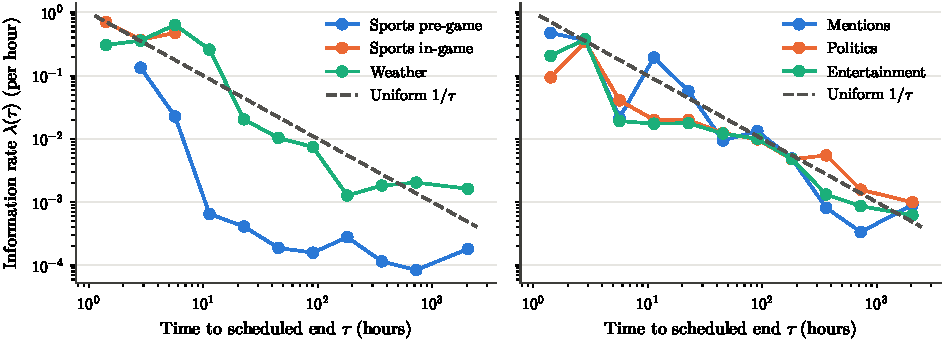
\includegraphics[width=\textwidth]{figures/fig_dyn_clock.pdf}
\caption{Information rate $\irate(\tauexp)$ per hour from the piecewise-constant clock fitted on the estimation sample (before 1 October 2026), against time to the scheduled end of information. The dashed line is the uniform clock $1/\tauexp$; buckets without data are omitted. In-game sports sit on the uniform clock; pre-game sports run one to two orders of magnitude below it; weather information is front-loaded into the final day.}
\label{fig:dyn-clock}
\end{figure}

\subsubsection{Distribution of innovations and jumps}\label{sec:dyn-res-shape}

\Cref{fig:dyn-u} contrasts the variance and the shape of $\ustd$. Once the clock is fitted,
$\Var(\ustd)$ is close to one by construction on the estimation sample. The shape, however, is far
from Gaussian everywhere except in-game.

Holdout excess kurtosis is 22 for weather and 59--1281 in the other non-sports
  categories and pre-game sports. With the fitted clock, $P(|\ustd|>4)$ is 0.7--2.7\% against
  0.006\% for a normal.
  % source: results_cat.json:categories.*.u_diag
Outside in-game sports (12\%), the mid does not change in 22\%
  (weather) to 85\% (Elections) of hours.
The EM mixture assigns 55--85\% of $\sum(\Delta\pr)^2$ to the jump
  component, with similar values in the estimation sample and the holdout (\cref{tab:dyn-sv}).
Outside in-game sports, the probability that a
  $|\ustd|>3$ hour is followed by another is 4.5--15\%, against an unconditional 1.4--4.7\%. Large moves cluster only mildly, so the
  tails are mainly isolated jumps rather than prolonged high-volatility episodes.
  % source: results_cat.json:categories.*.jumps.{big_after_big,big_uncond}

This matters for anyone using the model as a density. For contracts more than seven days from
their scheduled end in Mentions, Politics, Elections, Entertainment and Science \& Technology, the
Gaussian M0 overstates the mean one-hour $|\Delta\pr|$ by a factor of 2.1--3.4 across price groups.
The M2 mixture, which includes the zero-move mass, gives 0.7--1.2 times the realized value. Closer
to expiry, and for sports and weather, the two bracket the realized move.
% source: data/research/pm_vol/maker.json:economic (tau group >7d)

\begin{figure}[t]
\centering
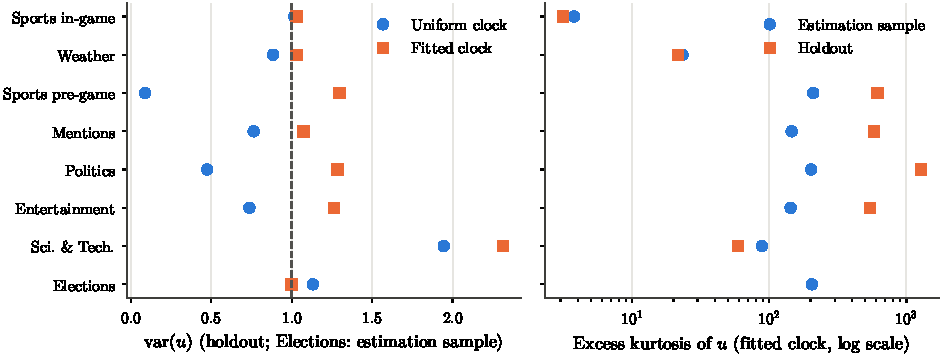
\includegraphics[width=\textwidth]{figures/fig_dyn_u.pdf}
\caption{Standardized innovations $\ustd$ (\cref{eq:dyn-u}) by category. Left: holdout (October 2026) variance under the uniform and the fitted clock; Elections has no holdout and shows the estimation sample. Right: excess kurtosis under the fitted clock, estimation sample and holdout, on a log scale. Only in-game sports are close to Gaussian.}
\label{fig:dyn-u}
\end{figure}

\subsubsection{Backbone}\label{sec:dyn-res-backbone}

\Cref{fig:dyn-backbone} plots squared price changes against the price level, after removing the
clock and quote noise.
Variance falls toward the edges more slowly than the probit backbone of M0
  implies, and far more slowly than the logit-normal backbone $[\pr(1-\pr)]^2$.
The QLIKE estimate of $\beta$ is 0.39 for pre-game sports, 0.47
  in-game, 0.58 for weather and 0.31--0.81 elsewhere. The Roll-corrected cell regression gives 0.44,
  0.49 and 0.54 for the same three categories in the estimation sample (\cref{tab:dyn-backbone}).

Logit-normal is rejected. It loses to probit on the estimation sample in every
  category ($t$ from 3.5 to 7.8, except Elections at 1.0). On the holdout it is worse in six of seven
  categories, significantly so in three (in-game $t=4.7$, weather $2.8$, Politics $2.4$).
Out of sample, the free-$\beta$ backbone beats probit in pre-game sports
  ($t=-1.7$), in-game ($-2.5$) and weather ($-1.8$), and loses in Entertainment ($+1.6$).
% source: results_cat.json:categories.*.backbone_table, beta_cells

Part of the extra volatility near the edges reflects the 1\cents{} tick: at $\pr=0.04$ a one-tick
move is large relative to $\varphi(\Phi^{-1}(\pr))$. The tick-grid control of
\cref{sec:dyn-res-drift} shows how much the grid alone distorts probit-unit statistics.

\begin{figure}[t]
\centering
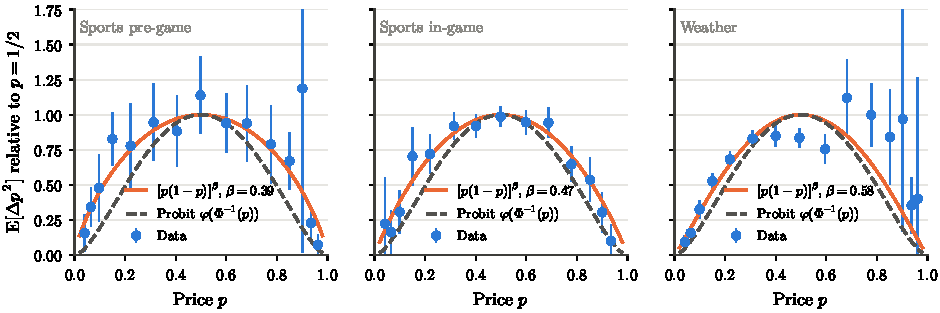
\includegraphics[width=\textwidth]{figures/fig_dyn_backbone.pdf}
\caption{Backbone. Points: mean of $[(\Delta \pr)^2-k s^2]/c_{j(\tauexp)}^2$ by price bin, estimation sample (before 1 October 2026), with $\pm2$ event-clustered standard errors; $c_j$ and $k$ are from the fitted power backbone, so the series is normalized to one at $\pr=1/2$. The solid line is the fitted $[\pr(1-\pr)]^{2\beta}$, normalized the same way; the dashed line is the probit backbone $\varphi(\Phi^{-1}(\pr))^2$ of M0. The logit-normal curve ($\beta=1$) lies below both and is omitted.}
\label{fig:dyn-backbone}
\end{figure}

\subsubsection{Stochastic volatility and leverage}\label{sec:dyn-res-sv}

\Cref{tab:dyn-sv} reports volatility clustering after the fitted clock is removed.
The within-market first-order autocorrelation of $|\ustd|$, which nets out
  static differences in volatility between markets, is 0.09--0.14 on the estimation sample ($t$ from
  2.0 to 6.4). It remains positive on the holdout, at 0.06--0.30.

The within-market half-life is 7--21 hours. The implied M1 vol-of-vol
  $\nu$ is 0.29--0.48 per $\sqrt{\text{day}}$. Weather is the exception, at 40 hours: its markets
  mostly live under 48 hours, so the within-market estimate rests on few markets.
Outside weather, the pooled autocorrelation decays more
  slowly, with half-lives of 21--29 hours; the difference is persistent heterogeneity in $\alpha$
  across markets.
% source: results_cat.json:categories.*.sv.{dev,holdout}.{acf_chosen,acf_within,fit_within,leverage,leverage_price_space}

The vol--price correlation $\rho$ is robust only in-game.
In-game, volatility rises after moves toward $1/2$: the correlation is $-0.11$
  ($t=-7.0$) on the estimation sample and $-0.08$ ($t=-4.2$) on the holdout in probit units, and
  $-0.14$ ($t=-8.8$) in price units.
Elsewhere the probit-unit correlation is indistinguishable from zero, except
  Entertainment and Science \& Technology ($+0.02$ and $+0.06$, $t\approx3$). The price-unit
  correlation is small and negative (weather $-0.03$, $t=-5.7$).
Because the sign depends on the units outside the in-game regime, we attribute it there to
backbone and tick mechanics rather than to a structural $\rho$. \Cref{sec:res-hf} shows that the
in-game effect is absent at minute scales.

\begin{table}[t]
\centering
\begin{threeparttable}
\caption{Stochastic volatility, leverage and jumps}\label{tab:dyn-sv}
\scriptsize
\setlength{\tabcolsep}{2.2pt}
% source: data/research/pm_vol/results_cat.json:categories.*.sv, jumps
\begin{tabular}{lccccccccc}
\toprule
 & \multicolumn{3}{c}{$\Corr(|\ustd_t|,|\ustd_{t+1}|)$} & Half-life & $\nu$ & \multicolumn{2}{c}{Leverage corr.\ ($t$)} & Jump share & Zero- \\
\cmidrule(lr){2-4}\cmidrule(lr){7-8}
Category & pooled & within ($t$) & within, hold. & (h) & per $\sqrt{\text{day}}$ & probit & price & est.\ / hold. & move \\
\midrule
Sports in-game & 0.12 & -- & 0.22 & -- & -- & $-0.109$ ($-7.0$) & $-0.144$ ($-8.8$) & 0.66 / 0.65 & 0.12 \\
Sports pre-game & 0.16 & 0.14 (6.4) & 0.21 & 9.4 & 0.48 & 0.001 (0.2) & $-0.009$ ($-2.2$) & 0.74 / 0.72 & 0.73 \\
Weather & 0.13 & 0.12 (2.0) & 0.30 & 40.1 & 0.16 & $-0.010$ ($-1.7$) & $-0.034$ ($-5.7$) & 0.62 / 0.55 & 0.22 \\
Mentions & 0.09 & 0.09 (5.5) & 0.06 & 6.8 & 0.44 & 0.006 (0.6) & $-0.003$ ($-0.3$) & 0.85 / 0.82 & 0.72 \\
Politics & 0.11 & 0.09 (4.6) & 0.28 & 11.6 & 0.33 & 0.009 (0.7) & $-0.031$ ($-2.4$) & 0.78 / 0.85 & 0.76 \\
Elections & 0.13 & 0.13 (3.5) & -- & 21.2 & 0.29 & $-0.001$ ($-0.1$) & $-0.023$ ($-1.5$) & 0.81 / -- & 0.85 \\
Entertainment & 0.11 & 0.09 (5.9) & 0.12 & 13.4 & 0.33 & 0.022 (3.2) & 0.006 (0.8) & 0.70 / 0.73 & 0.81 \\
Sci.\ \& Tech. & 0.14 & 0.10 (4.4) & 0.24 & 11.6 & 0.40 & 0.059 (3.5) & 0.021 (1.5) & 0.76 / 0.80 & 0.72 \\
\bottomrule
\end{tabular}
\begin{tablenotes}[flushleft]\footnotesize
\item Hourly $\ustd$ under the fitted clock. Estimation sample: before 1 October 2026; holdout: October 2026. Unless marked, statistics are from the estimation sample.
\item \emph{Within}: $|\ustd|$ demeaned by market, markets with at least 48 steps (in-game legs are too short). Half-life and $\nu$ come from the within-market fit $A\phi^k$, $k=1,\ldots,24$ (\cref{sec:dyn-sv}).
\item \emph{Leverage}: $\Corr(\sgn(\Zt_t)x_t,\,\tfrac16\sum_{j\le6}|x_{t+j}|)$ for $\pr\in[0.1,0.9]$, with $x=\ustd$ (probit) or $x=\Delta\pr$ over the backbone volatility (price); negative means volatility rises after moves toward $1/2$.
\item \emph{Jump share}: posterior-weighted share of $\sum(\Delta\pr)^2$ from the EM jump component (\cref{eq:dyn-em}). \emph{Zero-move}: share of hours without a mid change.
\item $t$ clustered by event.
\end{tablenotes}
\end{threeparttable}
\end{table}

\subsubsection{Forecasting realized variance}\label{sec:dyn-res-forecast}

\Cref{tab:dyn-forecast} compares the forecasts on the holdout.
Under QLIKE, M1 (fitted clock with the filtered
  vol state) beats \textsc{hist} in pre-game sports (one hour: $t=-6.0$; six hours: $t=-30.3$),
  weather ($-8.2$ and $-6.1$), in-game sports ($-3.0$) and Politics at one hour ($-2.2$).
The filtered state improves on M0 without it in pre-game
  sports ($t=-2.8$ and $-2.2$), in-game ($-3.1$), Politics at one hour ($-5.2$) and Mentions at six
  hours ($-2.2$).
M1 does not beat \textsc{hist} for Mentions, the category whose
  scheduled end drifts by about ten hours in October.

QLIKE and MSE disagree. Under MSE, M1 is never significantly better than M0 and is
  significantly worse in several cases (pre-game sports: $t=2.3$ and $4.2$). Down-weighting a quiet
  market pays under QLIKE, which penalizes under-prediction of small variances; MSE is dominated by
  the jumps that the filter cannot anticipate.
Replacing the probit backbone by the fitted power backbone (\textsc{m1bb}
  against M1, holdout QLIKE) helps only for pre-game sports at one hour ($t=-2.4$). It is worse in
  most other cases, for example weather at one hour ($t=5.4$).
% source: data/research/pm_vol/results_fc.json:forecast.tables

\begin{table}[t]
\centering
\begin{threeparttable}
\caption{Forecasting next-period realized variance (holdout)}\label{tab:dyn-forecast}
\footnotesize
\setlength{\tabcolsep}{3pt}
% source: data/research/pm_vol/results_fc.json:forecast.tables (split = holdout)
\begin{tabular}{lcrrccccccc}
\toprule
 & & & & \multicolumn{3}{c}{QLIKE difference ($t$)} & \multicolumn{2}{c}{MSE rel.\ to \textsc{hist}} & MSE \\
\cmidrule(lr){5-7}\cmidrule(lr){8-9}
Category & $H$ & Rows & Events & M1 $-$ \textsc{hist} & M1 $-$ M0 & M0 $-$ \textsc{hist} & M0 & M1 & M1$-$M0 ($t$) \\
\midrule
Sports in-game & 1 & 5{,}685 & 2568 & $-0.43$ ($-3.0$) & $-0.03$ ($-3.1$) & $-0.40$ ($-2.7$) & 0.32 & 0.32 & (1.2) \\
Sports pre-game & 1 & 208{,}130 & 3204 & $-0.58$ ($-6.0$) & $-0.56$ ($-2.8$) & $-0.01$ ($-0.1$) & 1.19 & 1.40 & (2.3) \\
Weather & 1 & 10{,}746 & 770 & $-0.36$ ($-8.2$) & $-0.11$ ($-1.9$) & $-0.26$ ($-3.4$) & 0.42 & 0.42 & (0.5) \\
Mentions & 1 & 13{,}781 & 36 & 0.96 (1.1) & $-0.36$ ($-1.4$) & 1.33 (1.5) & 0.96 & 0.97 & (0.1) \\
Politics & 1 & 16{,}106 & 83 & $-0.74$ ($-2.2$) & $-0.39$ ($-5.2$) & $-0.35$ ($-1.1$) & 0.57 & 0.79 & (1.7) \\
Entertainment & 1 & 28{,}394 & 56 & $-3.27$ ($-1.6$) & $-0.07$ ($-0.2$) & $-3.20$ ($-1.3$) & 0.94 & 0.97 & (1.4) \\
Sci.\ \& Tech. & 1 & 6{,}961 & 75 & $-0.28$ ($-2.1$) & 0.05 (0.4) & $-0.34$ ($-2.3$) & 0.10 & 1.02 & (2.8) \\
\addlinespace
Sports pre-game & 6 & 194{,}028 & 2854 & $-2.54$ ($-30.3$) & $-0.41$ ($-2.2$) & $-2.13$ ($-8.5$) & 0.40 & 0.85 & (4.2) \\
Weather & 6 & 3{,}873 & 546 & $-0.48$ ($-6.1$) & $-0.19$ ($-0.9$) & $-0.29$ ($-1.1$) & 0.33 & 0.34 & (3.3) \\
Mentions & 6 & 12{,}071 & 34 & 0.07 (0.3) & $-0.24$ ($-2.2$) & 0.31 (0.9) & 0.50 & 0.56 & (1.2) \\
Politics & 6 & 15{,}446 & 51 & $-0.70$ ($-1.6$) & $-0.23$ ($-1.0$) & $-0.47$ ($-1.2$) & 0.05 & 0.69 & (1.9) \\
Entertainment & 6 & 27{,}379 & 54 & $-4.45$ ($-1.5$) & $-0.15$ ($-0.7$) & $-4.30$ ($-1.3$) & 0.81 & 1.01 & (1.0) \\
Sci.\ \& Tech. & 6 & 5{,}451 & 65 & $-0.08$ ($-0.5$) & 0.01 (0.1) & $-0.09$ ($-0.6$) & 0.03 & 0.57 & (2.5) \\
\bottomrule
\end{tabular}
\begin{tablenotes}[flushleft]\footnotesize
\item Target: $RV_{t,H}=\sum_{j<H}(\Delta\pr_{t+j})^2$ (cents$^2$), $H$ in hours; decision rows with at least 24\,h of history. All forecasts, windows, EWMA half-lives and weights are calibrated on the estimation sample (before 1 October 2026); the table reports the holdout (October 2026). Elections has no holdout.
\item QLIKE differences are mean per-row loss differences (negative: the first model is better), $t$ clustered by event. MSE columns are holdout MSE relative to \textsc{hist}; the last column is the $t$-statistic of the per-row MSE difference M1 $-$ M0 (positive: M1 worse).
\end{tablenotes}
\end{threeparttable}
\end{table}

\paragraph{Economic significance.}
Spreads that are wide relative to the model's expected move do not mean that liquidity provision
earns its spread. Consider joining both sides of the best quotes every hour, with fills inferred
only from trades that print through the quote, positions held to settlement, and Kalshi maker fees.
This loses 1.25\cents{} per filled contract on the estimation sample ($t=-3.7$, 27{,}036 fills) and
1.56\cents{} on the holdout ($t=-4.0$, 17{,}055 fills). Restricting quotes to hours in which the
half-spread is at least 20 times the model's expected one-hour move, a threshold chosen on the
estimation sample, gives $+1.61$\cents{} per fill on the holdout ($t=0.7$, 350 fills). That is no
better than a plain half-spread filter of at least 10\cents{} with no model ($+1.70$\cents, $t=0.9$).
% source: data/research/pm_vol/maker.json:table
The cost to a liquidity provider is adverse selection on the fills that do trade through, not
diffusion risk, which the clock measures well. We do not pursue trading applications further.

\paragraph{Limitations.}
\begin{itemize}
\item The candle samples of the smaller categories were selected partly on volume, which affects
  the variance-identity ratios and limits the number of events.
\item Elections has no holdout because its October series have no prior schedule.
\item The Mentions schedule estimated on the \estim{} is about ten hours off in October.
\item Hourly candles cannot separate jumps from short bursts of stochastic volatility; the in-game
  L2 data in \cref{sec:res-hf} address this for sports.
\end{itemize}

\subsection{High-frequency in-game dynamics}\label{sec:res-hf}
% High-frequency in-game dynamics from the recorded L2 (two nights, 50 game legs).
% Every number traces to data/research/pm_vol/hf_results.json, drift_sim.json or drift_tail.json
% (written by src/albert/research/pm_vol.py; report research-pm-vol-hf-20261109T221912Z).

The in-game sample has 50 game-winner legs (NBA 14, NCAAF 14, NFL 10, NHL 12), with 6{,}965
in-game minutes over two nights (\cref{sec:dyn-hf}). % source: hf_results.json:games
Every statistic is reported next to the matched M0 control of \cref{sec:dyn-control}, which has the
same games, windows, starting prices and spreads but no jumps and no stochastic volatility. Five
facts emerge.
\begin{enumerate}
\item The variance scales like Brownian motion from one second to five minutes, at a level set by
  the league.
\item The mid shows no measurable bid--ask bounce, unlike a quote re-rounded to the tick each
  second.
\item The shape is far from Gaussian at seconds and becomes nearly Gaussian only at about five
  minutes, because about half of the variance arrives in jumps.
\item Jump sizes follow Stern's fixed-score scaling in basketball but not in football or hockey.
\item There is no vol--price correlation beyond what M0 implies at minute scales.
\end{enumerate}

\subsubsection{Scale invariance and the variance signature}\label{sec:dyn-res-hf-scale}

\Cref{tab:dyn-hf-m0} reports the standardized innovation under the uniform clock at each horizon.
Variance is flat in the horizon. $\Var(\ustd)$ is 0.71, 0.77, 0.77, 0.73 and 0.77 at
  1, 5, 15, 60 and 300 seconds, so the Brownian time scaling holds across two and a half orders of
  magnitude. The level is below one ($t$ of $\ustd^2-1$ between $-3.5$ and $-5.1$, by game). With
  start spreads of at most 2\cents{} it is 0.66--0.77.

The level is set by the league, and the per-league values are also flat in the
  horizon. NBA games run above the uniform clock ($\Var(\ustd)$ of 1.17--1.33); NCAAF (0.47--0.54),
  NFL (0.57--0.64) and NHL (0.57--0.67) run below it. A plausible reading is that the scheduled end
  is a poor proxy for the remaining game clock: long stoppages in football and the buffer in the
  scheduled expiration both make $\tauexp$ too long.

The shape is not scale-invariant. Excess kurtosis falls from 151 at one second to 51,
  24 and 9 at 5, 15 and 60 seconds, and to 2 at five minutes; $P(|\ustd|>4)$ falls from 0.99\% to
  zero.
The control behaves differently. In the matched control the tick grid inflates
  $\Var(\ustd)$ to 2.64 at one second, falling to 1.02 at one minute, and kurtosis stays below 7.
% source: hf_results.json:m0, m0_sim

\begin{table}[t]
\centering
\begin{threeparttable}
\caption{In-game M0 test by horizon: data and matched tick-grid control}\label{tab:dyn-hf-m0}
\scriptsize
\setlength{\tabcolsep}{3pt}
% source: data/research/pm_vol/hf_results.json:m0, m0_sim (start_spread_max_c = 3 unless noted)
\begin{tabular}{rrcccccccc}
\toprule
 & & \multicolumn{5}{c}{Data} & \multicolumn{3}{c}{M0 control (1\cents{} grid)} \\
\cmidrule(lr){3-7}\cmidrule(lr){8-10}
$h$ (s) & Steps & $\Var(\ustd)$ & ($t$) & Exc.\ kurt. & $P(|\ustd|>4)$, \% & $\Var(\ustd)$, 2\cents & $\Var(\ustd)$ & Exc.\ kurt. & $P(|\ustd|>4)$, \% \\
\midrule
1 & 319{,}821 & 0.71 & ($-5.1$) & 151.3 & 0.99 & 0.66 & 2.64 & 6.3 & 2.97 \\
5 & 63{,}909 & 0.77 & ($-3.6$) & 51.1 & 0.99 & 0.74 & 1.42 & 1.1 & 0.47 \\
15 & 21{,}277 & 0.77 & ($-3.6$) & 23.7 & 0.79 & 0.76 & 1.16 & 0.2 & 0.06 \\
60 & 5{,}265 & 0.73 & ($-4.4$) & 9.0 & 0.53 & 0.73 & 1.02 & 0.1 & 0.00 \\
300 & 991 & 0.77 & ($-3.5$) & 2.0 & 0.00 & 0.77 & 1.07 & 0.0 & 0.00 \\
\midrule
\multicolumn{10}{l}{\emph{By league (data): $\Var(\ustd)$ at $h=$ 1, 5, 15, 60, 300\,s; excess kurtosis at 1, 60, 300\,s}} \\
\multicolumn{2}{l}{NBA (14 games)} & 1.17 & 1.33 & 1.31 & 1.26 & 1.29 & 62.6 & 3.2 & 0.2 \\
\multicolumn{2}{l}{NCAAF (14)} & 0.47 & 0.48 & 0.49 & 0.48 & 0.54 & 161.3 & 9.9 & 1.8 \\
\multicolumn{2}{l}{NFL (10)} & 0.57 & 0.61 & 0.64 & 0.62 & 0.59 & 167.4 & 7.6 & 2.6 \\
\multicolumn{2}{l}{NHL (12)} & 0.65 & 0.65 & 0.65 & 0.57 & 0.67 & 309.9 & 24.1 & 4.4 \\
\bottomrule
\end{tabular}
\begin{tablenotes}[flushleft]\footnotesize
\item Recorded Kalshi L2, nights of 7--8 and 8--9 November 2026; one game-winner leg per game, 50 games. Non-overlapping $h$-second steps under the uniform clock to the scheduled end; start spread $\le3$\cents{} (``2\cents'': $\le2$\cents), mid in $[0.03,0.97]$; end spread $\le10$\cents.
\item ($t$): $t$-statistic of $\E[\ustd^2-1]$, clustered by game. The control simulates an M0 path per game and quotes it on the 1\cents{} grid with that game's spreads (\cref{sec:dyn-control}).
\item In the league rows, the columns under Data hold $\Var(\ustd)$ at the five horizons and the control columns hold the data's excess kurtosis at 1, 60 and 300\,s.
\end{tablenotes}
\end{threeparttable}
\end{table}

\Cref{fig:dyn-signature} shows the variance signature.
Realized variance of the mid per in-game hour is flat, between 453 and
  524\,c$^2$ for sampling intervals from 1 to 600 seconds. Fitting \cref{eq:dyn-signature} gives
  $\sigma^2=503$\,c$^2$ per hour and a noise variance at its lower bound of zero.
The control has the textbook signature: 1{,}148\,c$^2$ at one second,
  falling to 608 at one minute, with $\eta=0.27$\cents{} and noise accounting for 46\% of
  one-second realized variance.
% source: hf_results.json:signature, signature_fit, signature_sim, signature_fit_sim
Kalshi in-game mids therefore do not flicker across the tick. The book moves when the price moves,
and quote discreteness appears as stickiness rather than bounce. The slight rise of realized
variance from 1 to 10 seconds (453 to 524\,c$^2$) is mild positive autocorrelation at the seconds
scale: quotes take a few seconds to adjust. Beyond about ten seconds increments are uncorrelated.
For realized-variance estimation this means sparse sampling corrections
\citep{zhang2005,aitsahalia2005,hansenlunde2006} are unnecessary on this venue at these horizons.

\begin{figure}[t]
\centering
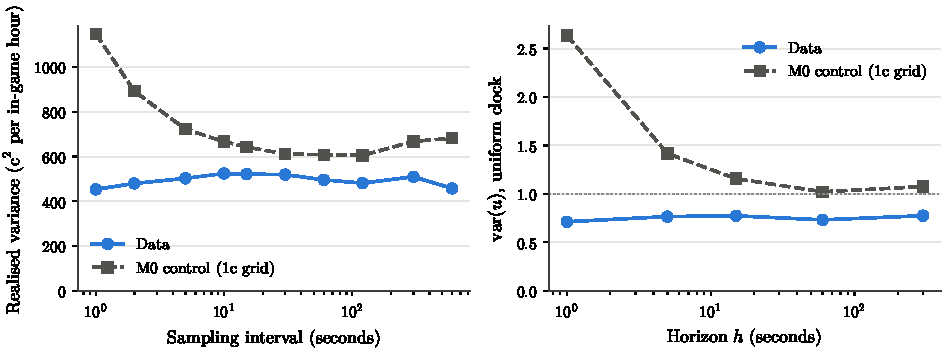
\includegraphics[width=\textwidth]{figures/fig_dyn_signature.pdf}
\caption{In-game variance signature and time scaling, recorded L2, two nights, 50 games. Left: realized variance of the mid per in-game hour against the sampling interval. Right: $\Var(\ustd)$ under the uniform clock against the horizon; the dotted line marks one. Dashed: the matched M0 control, quoted on the 1\cents{} grid with each game's own spreads.}
\label{fig:dyn-signature}
\end{figure}

\subsubsection{The probit-drift shortfall}\label{sec:dyn-res-drift}

In the hourly data the outward probit drift, which keeps $\pr$ a martingale under M0, is only a
fraction of its predicted size. The instrumental-variable estimates of \cref{sec:dyn-clock} are no
closer to one, so quote noise in $\Zt_t$ does not explain it. \Cref{tab:dyn-drift} and
\cref{fig:dyn-drift} test whether the price grid does.
In weather, Mentions, Elections and Science \& Technology,
  M0 paths quoted on the 1\cents{} grid with the real spreads reproduce the measured slope (data
  0.57, 0.42, 0.35, 0.47; tick control 0.32, 0.48, 0.37, 0.53). There the shortfall comes from the
  grid, the 0.5\cents{} probit clip and, for weather, the steep clock, which together truncate
  outward moves near the edges.
Ticks explain it only in part for Entertainment (0.35 against
  0.71) and Politics (0.73 against 1.03).

They do not explain it for sports: pre-game hourly
  0.11 ($\text{s.e.}=0.08$) against 0.93, and in-game L2 0.46 (0.21) at 60 seconds and 0.40 (0.25)
  at 300 seconds, against 1.37 and 0.87.
Stale quotes add nothing. Re-quoting only in hours with real activity gives the same
  slopes as the tick control.
% source: drift_sim.json (p_range = all); hf_results.json:drift_hf

Three further results locate the residual shortfall and rule out under-reaction as its source.
The price itself does not drift. The mean of $\sgn(\Zt_t)\Delta\pr$ is
  $+0.003$\cents{} per hour pre-game ($t=1.3$) and $-0.004$\cents{} per minute in-game ($t=-0.1$).
  A Gaussian M0 price with the measured Z-drift would drift by $-0.020$\cents{} per hour pre-game,
  which lies outside the confidence band of the measured value.
The shortfall is not in the tails. Trimming with windows that bias in opposite
  directions leaves the slope low: pre-game 0.13 and 0.05, in-game 0.68 and 0.61 at 60 seconds.
The core carries little of the clock. Within the core ($|\ustd|\le2$),
  $\E(\Delta\Zt)^2$ is only 8\% (pre-game), 19\% (Mentions, Entertainment) and 34\% (in-game, 60\,s)
  of the clock increment $L$. Within that core, the local second-order martingale ratio
  $\E[\sgn(\Zt)\Delta\Zt]/\E[\tfrac12|\Zt|(\Delta\Zt)^2]$ is 1.35--2.26.
% source: drift_tail.json

So the diffusive part of the motion drifts outward at least as much as a martingale requires given
its own variance. The shortfall arises because most of the clock's information arrives in jumps,
and the Gaussian compensator $e^{L/2}$ of M0 overstates the drift needed when the variance is
jump-borne. That is the M2 regime of \cref{sec:model}, not under-reaction. The only under-reaction
we find is the seconds-scale adjustment visible in the signature plot.

\begin{table}[t]
\centering
\begin{threeparttable}
\caption{Probit-drift slope: data, tick-grid controls and where the shortfall lies}\label{tab:dyn-drift}
\scriptsize
\setlength{\tabcolsep}{2.5pt}
% source: data/research/pm_vol/drift_sim.json (p_range = all), hf_results.json:drift_hf, drift_tail.json
\begin{tabular}{lcccccccc}
\toprule
 & \multicolumn{4}{c}{Slope (M0 $=1$)} & Trimmed slope & Core & Local & $\E[\sgn(\Zt)\Delta\pr]$ \\
\cmidrule(lr){2-5}
Sample & Data (s.e.) & Tick (s.e.) & Stale & True & $|\ustd|\le2$ / $|\Delta\Zt|\le2$sd & $\E(\Delta\Zt)^2/\E L$ & ratio & \cents{} ($t$) \\
\midrule
Weather (1\,h) & 0.57 (0.05) & 0.32 (0.01) & 0.28 & 0.57 & 0.69 / 0.62 & 0.49 & 1.35 & $-0.021$ ($-1.0$) \\
Mentions (1\,h) & 0.42 (0.12) & 0.48 (0.10) & 0.43 & 0.88 & 0.39 / 0.37 & 0.19 & 1.86 & 0.026 (1.5) \\
Elections (1\,h) & 0.35 (0.10) & 0.37 (0.12) & 0.34 & 0.84 & -- & -- & -- & 0.006 (1.6) \\
Sci.\ \& Tech.\ (1\,h) & 0.47 (0.16) & 0.53 (0.10) & 0.41 & 0.69 & -- & -- & -- & 0.026 (1.8) \\
Entertainment (1\,h) & 0.35 (0.15) & 0.71 (0.10) & 0.71 & 1.16 & 0.25 / 0.25 & 0.19 & 1.82 & $-0.003$ ($-0.9$) \\
Politics (1\,h) & 0.73 (0.11) & 1.03 (0.21) & 0.99 & 1.11 & 0.58 / 0.56 & 0.22 & 2.19 & $-0.010$ ($-0.9$) \\
Sports pre-game (1\,h) & 0.11 (0.08) & 0.93 (0.09) & 0.92 & 1.06 & 0.13 / 0.05 & 0.08 & 1.43 & 0.003 (1.3) \\
In-game L2 (60\,s) & 0.46 (0.21) & 1.37 (0.39) & -- & 1.29 & 0.68 / 0.61 & 0.34 & 2.26 & $-0.004$ ($-0.1$) \\
In-game L2 (300\,s) & 0.40 (0.25) & 0.87 (0.32) & -- & 0.93 & 0.51 / 0.47 & 0.48 & 1.35 & 0.031 (0.1) \\
\bottomrule
\end{tabular}
\begin{tablenotes}[flushleft]\footnotesize
\item Slope of $\tilde\Zt_{t+h}-\tilde\Zt_t$ on $\tilde\Zt_t(e^{L/2}-1)$, steps with $L\le2$. Hourly rows: estimation sample (before 1 October 2026), category clock fitted on the estimation sample. L2 rows: in-game, uniform clock. Standard errors clustered by event (hourly) or game (L2).
\item \emph{Tick}, \emph{Stale}, \emph{True}: M0 paths simulated on the same grids, quoted on the 1\cents{} grid with the real spreads, re-quoted only in hours with real activity, or not quoted (\cref{sec:dyn-control}).
\item \emph{Trimmed}: windows centred on M0's mean (biases toward 1) and on zero drift (biases toward 0). \emph{Core} and \emph{Local ratio}: within $|\ustd|\le2$; local ratio $=\E[\sgn(\Zt)\Delta\Zt]/\E[\frac12|\Zt|(\Delta\Zt)^2]$ on $|\Zt|\ge0.5$ (one for a martingale). The trimming diagnostics were run for the categories shown.
\item Last column: per hour (hourly rows) or per step (L2 rows), $t$ clustered as above.
\end{tablenotes}
\end{threeparttable}
\end{table}

\begin{figure}[t]
\centering
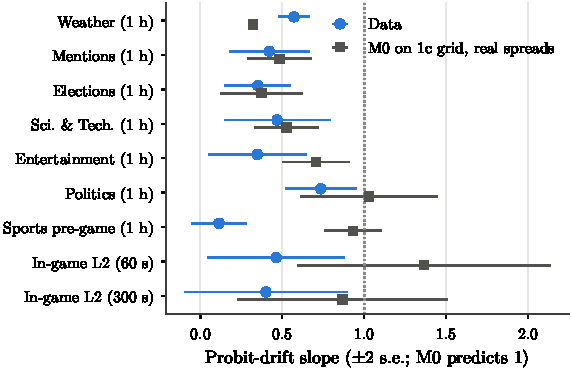
\includegraphics[width=0.66\textwidth]{figures/fig_dyn_drift.pdf}
\caption{Probit-drift slope ($\pm2$ standard errors, clustered by event or game) in the data and in M0 paths quoted on the 1\cents{} grid with the real spreads. Hourly rows: estimation sample (before 1 October 2026). L2 rows: in-game, two nights. The dotted line is M0's prediction. Ticks reproduce the shortfall in weather, Mentions, Elections and Science \& Technology but not in sports.}
\label{fig:dyn-drift}
\end{figure}

\subsubsection{Jumps and Stern's scaling}\label{sec:dyn-res-hf-jumps}

Panel A of \cref{tab:dyn-hf-jumps} measures how much of the in-game variance arrives in jumps.
Bipower variation misses 59\%, 53\% and 48\% of realized variance at 5, 10 and
  15 seconds; the median game shows 61--66\%. In the control, bipower variation misses only 8--16\%:
  the familiar small-sample and discreteness bias of bipower tests on a tick grid. The excess over
  the control, about 40--45 percentage points, is a conservative estimate of the in-game jump share.
Threshold jumps (more than four local standard deviations and at least 2\cents) carry
  51--68\% of realized variance, against 1\% or less in the control.
At 10 seconds we detect 859 jumps in 50 games, about 7.4 per
  in-game hour, with a median size of 3.5\cents. The control produces 58.
These shares are consistent with the hourly EM estimate for in-game sports (0.65--0.66 of
$\sum(\Delta\pr)^2$, \cref{tab:dyn-sv}).
% source: hf_results.json:jumps, jumps_sim, n_jumps_sim_10s, stern

For a fixed score increment, Stern's Brownian game model implies that the price jump scales as
$\varphi(\Zt)/\sqrt{\tauexp}$ (Panel B).
In the NBA the log--log slope is $1.08$ ($\text{s.e.}=0.09$), as predicted.

For the NFL, NCAAF and NHL the slope is 0.50 (0.10), 0.56 (0.08) and 0.65 (0.16); the
  pooled slope with league fixed effects is 0.69 (0.07).

Basketball scoring is frequent and small, close to the Brownian limit. Touchdowns, field goals and
goals are large and discrete, and their price impact depends on the game state through more than
$\varphi(\Zt)$. Measuring $\tauexp$ to the scheduled end rather than the game clock also flattens the
slope.

\subsubsection{Leverage at minute scales}\label{sec:dyn-res-hf-lev}

At horizons of one, two and five minutes (Panel C), the vol--price correlation in probit units is
$+0.016$, $+0.003$ and $+0.045$, all with $|t|<1.4$, matching the control's zero. In price units
the correlation is negative ($-0.056$ to $-0.088$). M0 itself produces this mechanically, because
$\varphi(\Zt)$ rises as the price moves toward $1/2$; the control gives $-0.07$ to $-0.17$. The
hourly in-game correlation of $-0.11$ in probit units (\cref{tab:dyn-sv}) therefore has no
counterpart at minute scales. If it is structural, it reflects game-state changes over hours, such
as the late stages of close games, rather than short-run feedback.
% source: hf_results.json:leverage, leverage_sim

\begin{table}[t]
\centering
\begin{threeparttable}
\caption{In-game jumps, Stern scaling and leverage}\label{tab:dyn-hf-jumps}
\footnotesize
\setlength{\tabcolsep}{3.5pt}
% source: data/research/pm_vol/hf_results.json:jumps, jumps_sim, stern, leverage, leverage_sim
\begin{tabular}{lccccc}
\toprule
\multicolumn{6}{l}{\emph{A. Share of realized variance from jumps}} \\
$h$ (s) & Bipower & Bipower, med.\ game & Bipower, control & Threshold & Threshold, control \\
\midrule
5 & 0.59 & 0.66 & 0.16 & 0.68 & 0.005 \\
10 & 0.53 & 0.61 & 0.09 & 0.57 & 0.009 \\
15 & 0.48 & 0.63 & 0.08 & 0.51 & 0.010 \\
\midrule
\multicolumn{6}{l}{\emph{B. Jump size against $\varphi(\Zt)/\sqrt{\tauexp}$, 10\,s jumps (Stern: slope 1)}} \\
League & Jumps & Games & Med.\ $|\Delta\pr|$ (\cents) & Price slope (s.e.) & Probit slope (s.e.) \\
\midrule
Pooled (league f.e.) & 859 & 50 & 3.5 & 0.69 (0.07) & 0.72 (0.10) \\
NBA & 236 & 14 & 4.0 & 1.08 (0.09) & 1.92 (0.12) \\
NCAAF & 187 & 14 & 3.5 & 0.56 (0.08) & 0.41 (0.14) \\
NFL & 284 & 10 & 3.5 & 0.50 (0.10) & 0.55 (0.11) \\
NHL & 152 & 12 & 3.0 & 0.65 (0.16) & 0.59 (0.21) \\
\midrule
\multicolumn{6}{l}{\emph{C. Leverage, \cref{eq:dyn-lev} with $x$ for $\ustd$ ($t$)}} \\
$h$ (s) & Steps & $x=\ustd$, data & $x=\ustd$, control & $x=\Delta\pr$, data & $x=\Delta\pr$, control \\
\midrule
60 & 4{,}447 & 0.016 (0.9) & 0.000 (0.0) & $-0.056$ ($-2.3$) & $-0.068$ ($-2.9$) \\
120 & 2{,}181 & 0.003 (0.1) & $-0.007$ ($-0.3$) & $-0.088$ ($-2.8$) & $-0.106$ ($-3.5$) \\
300 & 822 & 0.045 (1.4) & 0.008 (0.2) & $-0.075$ ($-1.7$) & $-0.165$ ($-4.7$) \\
\bottomrule
\end{tabular}
\begin{tablenotes}[flushleft]\footnotesize
\item Recorded L2, two nights, 50 games; steps with start spread $\le3$\cents{} and mid in $[0.03,0.97]$ (Panel C: $[0.1,0.9]$). Control: M0 paths quoted on the 1\cents{} grid with each game's spreads.
\item A: bipower share $=(RV-BV)/RV$; threshold jumps have $|\ustd|>4$ local bipower standard deviations and $|\Delta\pr|\ge2$\cents. B: price slope of $\log|\Delta\pr|$ on $\log[\varphi(\Zt)/\sqrt{\tauexp}]$; probit slope of $\log|\Delta\Zt|$ on $\log\tauexp^{-1/2}$; OLS, standard errors clustered by game. C: correlation of $\sgn(\Zt_t)x_t$ with the mean $|x|$ over the next five steps; $t$ clustered by game; negative values mean volatility rises after moves toward $1/2$.
\end{tablenotes}
\end{threeparttable}
\end{table}

\paragraph{Limitations.}
\begin{itemize}
\item The sample covers two nights and 50 games, so league-level estimates rest on 10--14 games
  each.
\item The in-game window comes from the schedule and can include a few pre-kickoff minutes, which
  pushes $\Var(\ustd)$ down.
\item $\tauexp$ is measured to the scheduled settlement time, not the game clock.
\item Without a score feed, ``jumps'' are price discontinuities, not verified scoring events.
\end{itemize}

\subsection{Strike ladders: the prediction-market smile}\label{sec:res-lad}
% Strike ladders: results. All numbers from data/research/pm_smile/summary.json (written by
% albert.research.pm_smile analyze, report data/reports/research-pm-smile-20261109T220959Z) unless
% a comment says otherwise. Figures: paper/scripts/fig_ladders.py.

\paragraph{Sample.}
The fitted sample has 24,192 snapshots of 10,177 ladders in 9,213 events from 309 series, priced
from 232,594 leg quotes. There are 12,627 snapshots in the \estim{} and 11,565 in the holdout.
% source: summary.json:coverage (column sums); snapshots.parquet (series count)
Sports ladders account for 16,342 snapshots and weather for 7,271. Politics (270 snapshots),
entertainment (207), science and technology (57) and other climate series (44) are small.
\Cref{tab:lad-sample} in \cref{app:lad} gives coverage by group. Most attrition comes from legs
without a recent candle or with a spread above 5\cents. Among weather lows, where the middle
brackets are often quoted wider than 5\cents, it also comes from incomplete bracket sets.
% source: summary.json:build_stats

\subsubsection{The shape of the smile}

Every group has a smile (\cref{tab:lad-smile,fig:lad-smile}): the curvature $c$ in
\eqref{eq:lad-smile} is positive, with a 95\% interval excluding zero, in every group, lead and
sample. Implied wings are therefore fatter than a normal distribution with
the ATM width. The skew differs by underlying.
\begin{itemize}
\item \emph{Sports totals and team totals} are right-skewed, $s=0.071$ and $0.046$ six hours
  before expiry. Upper-wing volatilities exceed lower-wing ones, as for a count bounded below.
\item \emph{Spreads}, oriented to the favourite, are nearly symmetric ($s=0.010$).
\item \emph{Weather highs and lows} carry a small left skew ($s=-0.017$ and $-0.031$).
\item \emph{Politics} ladders have no significant skew and a curvature of about 0.07, at the upper
  end of the range (weather lows and entertainment reach 0.087 and 0.088).
\end{itemize}
The pooled curvature at a given lead is stable across leads: weather highs give
$c=0.054$--$0.055$ at every lead from 36 to 16 hours (\cref{tab:lad-smile-full}).
% source: summary.json:smile (split "both")
The median per-snapshot curvature is smaller than the pooled one for sports, for example
$-0.005$ against $0.014$ for totals at six hours. The pooled curvature is driven by the far wings,
where (\cref{fig:lad-smile}) the volatility ratio rises steeply beyond $|m|\approx2$. Part of that
rise is mechanical: a wing quoted at the 1\cents{} tick has an implied volatility that grows with
$|m|$ whatever the true tail.

\begin{table}[t]
\centering\footnotesize
\setlength{\tabcolsep}{2.8pt}
\begin{threeparttable}
\caption{Implied smile and density shape by ladder group.}\label{tab:lad-smile}
% source: summary.json:smile (split "both", lead as shown); summary.json:jf_shapes (lead_h = -1)
\begin{tabular}{@{}llcccccc@{}}
\toprule
 & & \multicolumn{2}{c}{Smile, \eqref{eq:lad-smile}} & \multicolumn{2}{c}{Bowley skewness} & \multicolumn{2}{c}{Tail weight} \\
\cmidrule(lr){3-4}\cmidrule(lr){5-6}\cmidrule(lr){7-8}
Group & Lead & $s$ ($t$) & $c$ ($t$) & Estimation & Holdout & Estimation & Holdout \\
\midrule
Weather highs & 24 h & $-0.017$ ($-14.4$) & 0.055 (62.2) & $-0.015$ / $-0.077$ & $-0.020$ / $-0.033$ & 1.290 / 1.050 & 1.231 / 1.044 \\
Weather lows  & 36 h & $-0.031$ ($-5.3$) & 0.067 (18.1) & -- & -- & -- & -- \\
Sports totals & 6 h  & 0.071 (66.3) & 0.014 (12.6) & 0.123 / 0.116 & 0.101 / 0.067 & 1.184 / 1.082 & 1.200 / 1.030 \\
Team totals   & 6 h  & 0.046 (30.0) & 0.023 (18.7) & 0.095 / 0.070 & 0.054 / 0.028 & 1.395 / 1.075 & 1.245 / 1.057 \\
Spreads       & 6 h  & 0.010 (4.4) & 0.041 (8.9) & 0.035 / 0.035 & 0.002 / 0.026 & 1.364 / 1.190 & 1.129 / 1.055 \\
Politics      & 6 h  & 0.008 (0.8) & 0.070 (18.1) & 0.008 / 0.074 & 0.031 / $-0.036$ & 2.588 / 1.422 & 2.605 / 1.161 \\
\bottomrule
\end{tabular}
\begin{tablenotes}[flushleft]\footnotesize
\item Smile: pooled least squares of $\sigma_K/\satm-1$ on $(1,m,m^2)$ over off-ATM strikes at the
lead shown, estimation sample (before 1 October 2026) and holdout (October 2026) pooled; $t$
clustered by event. All leads, samples and 95\% intervals are in \cref{tab:lad-smile-full}.
Bowley skewness and tail weight (1 for a normal) come from Jones--Faddy skew-$t$ fits in
standardised units over all leads; each cell is implied / realised. Implied fits use the pooled
survival points; realised fits are interval-censored maximum likelihood on $(X_T-\Fmed)/\satm$.
Cluster-bootstrap 90\% intervals of the implied tail weight are at most 0.08 wide in the
sports and weather-high cells. Weather-low skew-$t$ fits are unstable (implied tail weight 2.59
in the estimation sample and 1.02 in the holdout) and are omitted.
\end{tablenotes}
\end{threeparttable}
\end{table}

\begin{figure}[t]
\centering
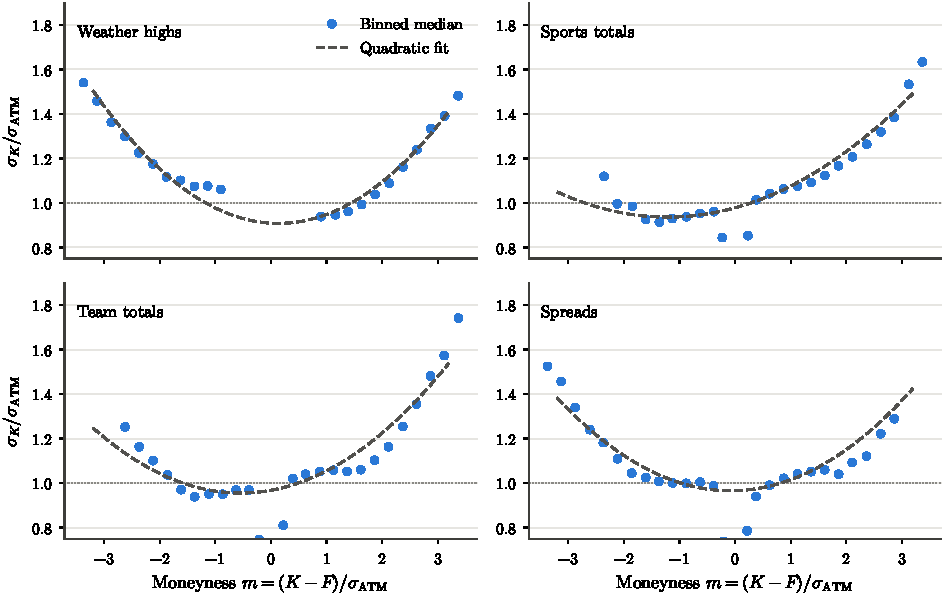
\includegraphics[width=\textwidth]{figures/fig_lad_smile.pdf}
\caption{Implied volatility smile. Median $\sigma_K/\satm$ in moneyness bins of width 0.25 (bins
with at least 30 strikes), all leads and both samples pooled, with the pooled quadratic fit of
\eqref{eq:lad-smile}. The dotted line is the flat smile of a normal implied distribution. Bins
near $m=0$ are noisy because $\sigma_K=(\Fmed-K)/\Phi^{-1}(S)$ has a small denominator there.}
\label{fig:lad-smile}
\end{figure}

The skew-$t$ summaries compare like with like (\cref{tab:lad-smile}, last four columns). The
implied skew has the right sign and roughly the right size. For sports totals the implied Bowley
skewness is 0.123 and 0.101 in the two samples, against 0.116 and 0.067 realised. Weather highs
are left-skewed in both the implied and the realised fits. Implied tails, however, are
consistently heavier than realised ones. The implied tail weight is 1.13--1.40 for sports and
1.23--1.29 for weather highs, against 1.03--1.19 and 1.04--1.05 realised. That gap is the
cross-strike form of the favourite--longshot bias~\citep{griffith1949,thalerziemba1988,snowbergwolfers2010}.

\subsubsection{Smile dynamics: sticky moneyness, not sticky strike}

\Cref{tab:lad-dyn} reports the regressions \eqref{eq:lad-atm}--\eqref{eq:lad-fixedk} on
consecutive snapshot pairs. Two pieces of evidence reject a sticky-strike smile.

\emph{The ATM point does not slide along the smile.} When the median moves, $\satm$ barely
responds. The slope $b$ is 0.017 for sports totals, $-0.031$ for team totals, $-0.020$ for spreads
and $-0.040$ for weather highs. A smile fixed in strike would give the pooled skew instead (0.065,
0.039, 0.013 and $-0.014$). Using each snapshot's own skew, the coefficient $\delta$ that should
equal 1 under sticky strike is between 0.06 and 0.54 in the weather and sports groups, and $\delta=1$ is rejected at $|t|\ge4.1$ for
totals, team totals and weather highs.

\emph{The volatility at a fixed strike moves with the median} (\cref{fig:lad-sticky}). With the
pooled smile, the sticky-moneyness coefficient $\gamma$ is 1.01 for spreads, 1.17 for weather highs,
1.31 for totals and 2.11 for team totals ($t$ from 9 to 25 against zero). Sticky strike ($\gamma=0$)
is rejected in every group. For totals and team totals the coefficient also exceeds one: the
smile moves more than one-for-one with the median, possibly because the wings re-price as the
game state changes.

The raw response has the sign sticky moneyness predicts. In sports totals, where $s>0$, the
volatility at a fixed strike falls when the median rises: $-0.081$ per unit of $\Delta\Fmed_n$
($t=-15.9$). With each snapshot's own smile the coefficients fall to 0.25--0.63 in sports,
consistent with attenuation from measurement error in snapshot-level $(s,c)$. Weather highs, whose
snapshot smiles are better determined, give 1.17 under either definition.
% source: summary.json:dynamics_atm, dynamics_fixed_strike

\begin{table}[t]
\centering\footnotesize
\setlength{\tabcolsep}{2.4pt}
\begin{threeparttable}
\caption{Smile dynamics between consecutive snapshots.}\label{tab:lad-dyn}
% source: summary.json:dynamics_atm and summary.json:dynamics_fixed_strike
\begin{tabular}{@{}lrccccccc@{}}
\toprule
 & & \multicolumn{2}{c}{ATM, \eqref{eq:lad-atm}} & \multicolumn{3}{c}{Fixed strike, \eqref{eq:lad-fixedk}} & \multicolumn{2}{c}{Backbone $\beta$} \\
\cmidrule(lr){3-4}\cmidrule(lr){5-7}\cmidrule(lr){8-9}
Group & Pairs & $b$ ($t$) & $\bar s$ & $\gamma$ pooled ($t_{\gamma=1}$) & $\gamma$ snapshot & $\partial\sigma_K/\partial\Fmed$ ($t$) & Within ($t$) & Cross ($t$) \\
\midrule
Weather highs & 4,230 & $-0.040$ ($-7.4$) & $-0.014$ & 1.17 (3.6) & 1.17 & 0.019 (2.0) & -- & -- \\
Sports totals & 3,984 & 0.017 (1.4) & 0.065 & 1.31 (4.5) & 0.63 & $-0.081$ ($-15.9$) & 0.28 (3.2) & 0.29 (13.2) \\
Team totals   & 2,566 & $-0.031$ ($-2.8$) & 0.039 & 2.11 (10.1) & 0.30 & $-0.117$ ($-14.1$) & $-0.12$ ($-2.9$) & 0.22 (13.8) \\
Spreads       & 2,250 & $-0.020$ ($-1.5$) & 0.013 & 1.01 (0.1) & 0.25 & $-0.003$ ($-0.4$) & -- & -- \\
Politics      & 155   & $-0.056$ ($-0.8$) & 0.017 & 0.68 ($-2.5$) & 0.33 & 0.055 (1.8) & 0.69 (1.2) & 0.20 (1.9) \\
\bottomrule
\end{tabular}
\begin{tablenotes}[flushleft]\footnotesize
\item Pairs of consecutive snapshots of one ladder, estimation sample (before 1 October 2026) and
holdout (October 2026) pooled. Fixed effects for each group and lead pair; $t$ clustered by event.
$b$: slope of $\Delta\satm/\satm$ on $\Delta\Fmed/\satm$. $\bar s$: mean pooled skew, the
sticky-strike prediction for $b$ (sticky moneyness predicts 0). The coefficient $\delta$ on
$s\,\Delta\Fmed/\satm$ with each snapshot's skew (1 under sticky strike) is 0.23, 0.06, 0.12, 0.54
and $-0.31$ in the five rows ($t_{\delta=1}=-4.9$, $-4.1$, $-5.3$, $-1.3$, $-6.4$). $\gamma$: coefficient
on the sticky-moneyness prediction $-(s+2cm)\Delta\Fmed/\satm$, using the group-and-lead pooled
smile or each snapshot's own smile (1 under sticky moneyness, 0 under sticky strike); the pooled
$\gamma$ has $t$ between 9.4 and 24.6 against zero (5.3 for politics). Fixed-strike pairs: 5,259
(weather highs), 28,108 (totals), 16,490 (team totals), 24,867 (spreads), 730 (politics).
$\partial\sigma_K/\partial\Fmed$: raw slope of the fixed-strike change on $\Delta\Fmed/\satm$.
Backbone: $\Delta\log\satm$ on $\Delta\log\Fmed$ within ladders, and $\log\satm$ on $\log\Fmed$
with series-by-lead fixed effects, for positive underlyings only.
\end{tablenotes}
\end{threeparttable}
\end{table}

\begin{figure}[t]
\centering
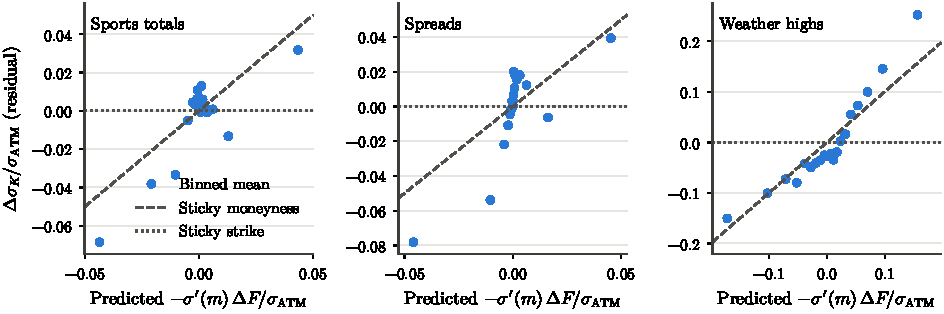
\includegraphics[width=\textwidth]{figures/fig_lad_sticky.pdf}
\caption{Fixed-strike volatility change against the sticky-moneyness prediction
$-\sigma'(m)\,\Delta\Fmed/\satm$ (pooled smile), after removing group-by-lead-pair means and
partialling out the level term of \eqref{eq:lad-fixedk}. Points are means in 20 quantile bins
of the prediction. Sticky moneyness predicts the dashed 45-degree line, sticky strike the dotted
zero line. In sports most pairs have small median moves; the slope is identified by the
larger moves.}
\label{fig:lad-sticky}
\end{figure}

\emph{Backbone.} For sports totals, $\satm$ rises with the level of the median both across games
($\beta=0.29$, $t=13.2$) and within a game between snapshots ($\beta=0.28$, $t=3.2$). Both are
well below the square-root exponent $\tfrac12$ of a Poisson count. For team totals the cross-section gives
$\beta=0.22$ but the within-game exponent is slightly negative ($-0.12$). The SABR-style level
backbone is therefore weak: the volatility of a ladder is set mainly by its moneyness and its
clock, not by the level of the underlying.

\subsubsection{ATM term structure}

\Cref{fig:lad-termstructure} plots $\log\satm$ against the lead within ladders. The estimated
exponents $\eta$ (\cref{tab:lad-term}) separate three information clocks.
% source: summary.json:term_structure
\begin{itemize}
\item \emph{Weather highs} have $\eta=0.773$ [0.760, 0.786], well above the uniform-clock value
  $\tfrac12$. Uncertainty about the daily maximum resolves late, during the afternoon of the
  measurement day.
\item \emph{Weather lows} have $\eta=0.480$ [0.413, 0.546], indistinguishable from $\tfrac12$.
  Their profile is flat from 16 to 8 hours, after the morning minimum has been observed.
\item \emph{Politics, entertainment and science} ladders are sub-diffusive (0.35, 0.19 and 0.24).
  Their information arrives in lumps close to resolution.
\item \emph{Sports ladders} have no pre-game time decay at all ($\eta=0.001$--$0.009$): nothing is
  learned about the score before the game starts.
\end{itemize}

\begin{figure}[t]
\centering
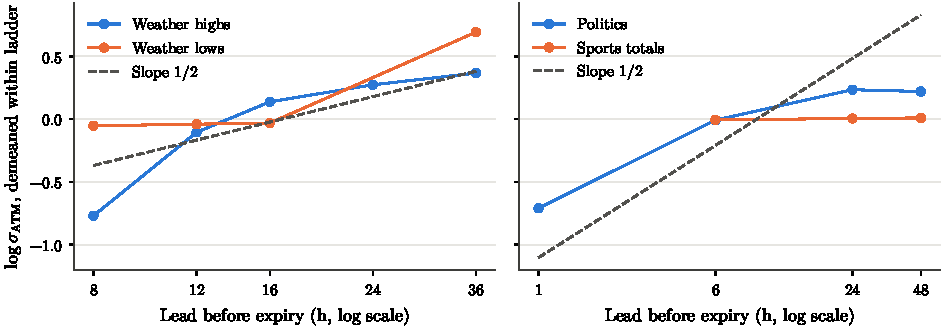
\includegraphics[width=\textwidth]{figures/fig_lad_termstructure.pdf}
\caption{ATM term structure. Mean of $\log\satm$, demeaned within ladder, by lead before expiry
(log scale). Left: weather highs and lows (hours before the measurement-day close). Right: politics and
sports totals (hours before the expected expiration; sports pre-game leads only). The dashed line
has slope $\tfrac12$, the uniform information clock.}
\label{fig:lad-termstructure}
\end{figure}

\subsubsection{Calibration against the realised outcome}

\Cref{tab:lad-calib} and \cref{fig:lad-calibration} test the implied distribution against
$X_T$. Sports ladders are calibrated in width and shape. In the holdout the width ratio is 1.02--1.03
(no $|t|$ above 1.1). The fractional PIT histogram is flat, with outer-decile shares of 0.192--0.202
against 0.2. In the \estim{} the widths are slightly too narrow (totals 1.045, $t=2.2$; spreads
1.144, $t=4.0$), and spreads put too much mass in the outer deciles (0.234); neither carries over
to the holdout.

Weather is too wide. The width ratio for highs is 0.941 ($t=-2.4$) and 0.890 ($t=-3.8$), and the
PIT puts too little mass in the outer deciles for both highs and lows (0.168--0.180, $t$ from
$-3.2$ to $-6.3$). Sports totals show a location bias: the realised total lands above the implied
median by $0.121\,\satm$ in the \estim{} ($t=5.1$) and $0.064\,\satm$ in the holdout ($t=2.4$).
% source: summary.json:width (lead_h = -1), summary.json:pit

The tail-mass comparison (\cref{fig:lad-calibration}, right; \cref{tab:lad-tails}) locates the
excess width in the wings.
\begin{itemize}
\item \emph{Weather highs.} Beyond $|m|\ge2.5$ the market prices 0.93--1.11\cents{} of tail mass
  per strike; realised frequencies are 0--0.30\cents{} ($z_{H_0}$ between $-0.5$ and $-2.6$, all
  negative).
\item \emph{Weather lows.} Every wing and threshold has $z_{H_0}<0$.
\item \emph{Sports.} The evidence is mixed. Holdout upper tails of totals at $|m|\ge2.5$ are
  overpriced (1.70\cents{} implied, 0.11\cents{} realised, $z_{H_0}=-2.2$), but the same cell in the
  \estim{} is not (1.77 against 2.19\cents).
\item \emph{Politics and entertainment.} Beyond $|m|\ge1.5$, wings are priced at 0.8--3.3\cents{} and
  are realised less often in most cells, but with at most 64 events per cell no $z_{H_0}$ is below
  $-1.3$.
\end{itemize}
% source: summary.json:tail_summary

\begin{table}[t]
\centering\small
\setlength{\tabcolsep}{4pt}
\begin{threeparttable}
\caption{Calibration of the implied distribution against the realised outcome.}\label{tab:lad-calib}
% source: summary.json:width (lead_h = -1) and summary.json:pit
\begin{tabular}{@{}lcccccc@{}}
\toprule
 & \multicolumn{2}{c}{Width ratio $\lambda$ ($t_{\lambda=1}$)} & \multicolumn{2}{c}{Location $\mu$ ($t$)} & \multicolumn{2}{c}{PIT outer-decile share ($t_{0.2}$)} \\
\cmidrule(lr){2-3}\cmidrule(lr){4-5}\cmidrule(lr){6-7}
Group & Estimation & Holdout & Estimation & Holdout & Estimation & Holdout \\
\midrule
Weather highs & 0.941 ($-2.4$) & 0.890 ($-3.8$) & 0.066 (1.9) & $-0.095$ ($-2.4$) & 0.178 ($-3.2$) & 0.170 ($-3.9$) \\
Weather lows  & 0.916 ($-0.7$) & 0.949 ($-0.7$) & $-0.081$ ($-1.5$) & 0.064 (0.8) & 0.168 ($-6.3$) & 0.180 ($-3.5$) \\
Sports totals & 1.045 (2.2) & 1.021 (1.0) & 0.121 (5.1) & 0.064 (2.4) & 0.196 ($-0.6$) & 0.192 ($-0.9$) \\
Team totals   & 1.045 (1.6) & 1.025 (1.0) & 0.127 (3.7) & 0.021 (0.6) & 0.199 ($-0.1$) & 0.202 (0.2) \\
Spreads       & 1.144 (4.0) & 1.027 (1.1) & 0.000 (0.0) & $-0.047$ ($-1.5$) & 0.234 (2.7) & 0.201 (0.1) \\
Politics      & 1.216 (1.0) & 1.297 (1.8) & $-0.152$ ($-0.9$) & 0.052 (0.3) & 0.192 ($-0.2$) & 0.233 (0.9) \\
Entertainment & 1.179 (1.9) & 0.852 ($-1.6$) & 0.013 (0.1) & 0.056 (0.3) & 0.205 (0.2) & 0.164 ($-2.8$) \\
\bottomrule
\end{tabular}
\begin{tablenotes}[flushleft]\footnotesize
\item One observation per snapshot, all leads pooled; estimation sample (before 1 October 2026),
holdout (October 2026). $\lambda$, $\mu$: interval-censored normal maximum likelihood for
$(X_T-\Fmed)/\satm$; $\lambda<1$ means the implied ATM width is too wide. PIT: fractional
histogram of the interval-censored probability integral transform; share of mass in the deciles
$[0,0.1)$ and $[0.9,1]$, 0.2 under calibration. All $t$ statistics cluster by event. Spread
locations are in the favourite's orientation.
\end{tablenotes}
\end{threeparttable}
\end{table}

\begin{figure}[t]
\centering
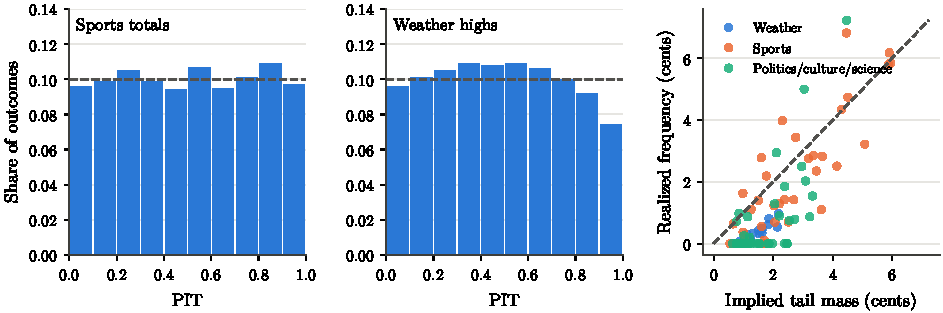
\includegraphics[width=\textwidth]{figures/fig_lad_calibration.pdf}
\caption{Calibration. Left and centre: fractional PIT histograms in the holdout (October 2026) for
sports totals and weather highs; the dashed line is the uniform density. Right: implied tail mass
against realised frequency, per group, sample, wing and threshold $|m|\ge1,\dots,2.5$ (thresholds
from 1.5 shown), in cents; the dashed line is calibration.}
\label{fig:lad-calibration}
\end{figure}

\subsubsection{Implied versus realised variance between snapshots}

\Cref{fig:lad-variance} and \cref{tab:lad-variance} report the ratio \eqref{eq:lad-vr}.
% source: summary.json:variance_between
\emph{Sports, pre-game.} Both terms are nearly zero, since neither the median nor the width moves,
and the ratio is not informative.
\emph{Sports, in play} (6 hours to 1 hour before expiry). Realised variance falls short of the
implied variance drop:
\begin{itemize}
\item totals 0.90 [0.81, 0.98];
\item spreads 0.92 [0.84, 1.04];
\item team totals 0.65 [0.59, 0.70].
\end{itemize}
The implied distribution narrows faster than its median moves: a variance premium, sizeable only
for team totals.

\emph{Weather highs} change sign across the day. The ratio is 1.02 from 36 to 24 hours, 0.66
[0.58, 0.73] overnight (24 to 16 hours) and 1.08 in the morning (16 to 12 hours). It reaches 1.55
[1.37, 1.74] in the afternoon (12 to 8 hours), when the median moves more than the narrowing of
the distribution allows. The weather median is also not a martingale. Its standardised drift is
$-0.046$ overnight ($t=-4.5$) and positive in the other three windows ($t$ from 2.8 to 5.8): the
market under-forecasts the daytime maximum until observations arrive.

\begin{figure}[t]
\centering
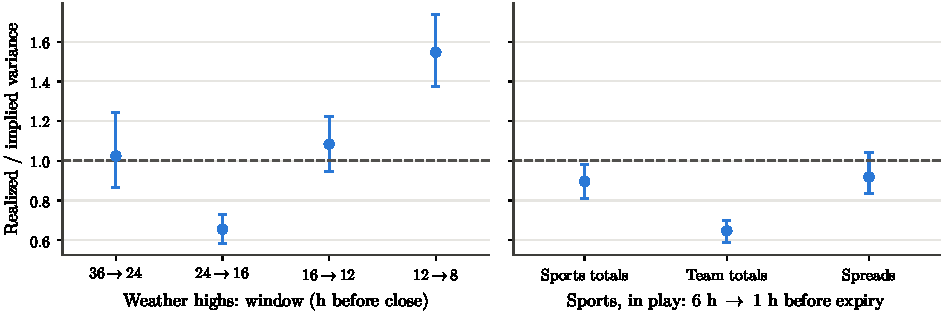
\includegraphics[width=\textwidth]{figures/fig_lad_variance.pdf}
\caption{Realised over implied variance between consecutive snapshots, \eqref{eq:lad-vr}, with
90\% cluster-bootstrap intervals over events. Left: weather highs by window (hours before the
measurement-day close). Right: sports ladders in play, 6 to 1 hours before the expected
expiration. The dashed line is equality.}
\label{fig:lad-variance}
\end{figure}

\subsubsection{Economic significance}

The wing premium is small in money terms.
% source: summary.json:pooled_rules (scope "all groups")
\begin{itemize}
\item \emph{Gating by model moneyness.} Selling the tail side of every leg with model moneyness
  $|m|\ge2.5$ at the snapshot quote, after the taker fee, returns $+0.23\cents$ per contract in the
  \estim{} ($t_{\text{risk}}=0.4$, 2,741 contracts) and $+1.10\cents$ in the holdout
  ($t_{\text{risk}}=2.0$, 3,006 contracts).
\item \emph{Gating by price alone.} The control (tail price at most 2\cents) returns $+0.31$ and
  $+0.25\cents$.
\item \emph{Within one price band.} Among tails priced at most 5\cents, legs with $|m|\ge2$ return
  $+0.29$ and $+0.49\cents$ while legs with $|m|<2$ return $-1.22$ and $-0.85\cents$: moneyness
  separates the overpriced wings from the rest.
\end{itemize}
The gain per contract is bounded by the 1\cents{} tick, and the evidence is weak once
settlement risk is taken into account. Net-of-fee arbitrage between legs (monotonicity or bracket
sums) appears in 30 of 24,192 snapshots. % source: summary.json:arbitrage (sums)

\subsubsection{Limitations}

Several limitations apply.
\begin{itemize}
\item \emph{Quotes.} They are hourly candle closes up to two hours old, without displayed size, and
  closes of different legs are not synchronous.
\item \emph{Spread filter.} The 5\cents{} filter discards many weather-low bracket sets and most
  far wings that have no bid.
\item \emph{Tick floor.} Wings quoted at the 1\cents{} tick inflate far-wing volatilities, so part of
  the measured curvature is a price-grid effect.
\item \emph{Interval censoring.} The realised outcome is known only up to the bracket containing
  it. This limits the precision of the realised skew-$t$ fits, which carry no intervals.
\item \emph{Fixed-strike coefficient.} With snapshot smiles it is attenuated by measurement error.
  With pooled smiles it inherits any misspecification of a common smile within a group and lead.
\item \emph{Sports clock.} The expected expiration of sports markets is a scheduled time, so the
  1 hour snapshot falls at different stages of different games.
\item \emph{Multiple comparisons.} We report many groups, leads and tests. The statements above
  rely on patterns that recur across groups or samples rather than on single cells.
\end{itemize}

\subsection{Deadline contracts: hazard term structures and theta}\label{sec:res-haz}
% Deadline contracts: results. Every number is taken from the saved study outputs:
% data/research/pm_hazard/summary.json (keys noted next to each table and key number).

\subsubsection{Implied hazards are too high, most of all in the last day}\label{haz-res-calib}

\Cref{haz-tab-calib} reports the hazard multiplier $k$ of \cref{haz-eq-k} for the pooled event,
mention and count contracts, by lead and split. In the \estim{} the implied hazard is too high at
every lead. Realised hazards are about 61\% of implied ones within a day of the deadline and 61--79\%
at longer leads, and every 90\% interval lies below one. In cents, prices exceed realised frequencies
by 1.2--8.6\cents{} per contract, and the gap grows with the lead because longer windows carry
higher prices. The holdout confirms the near-deadline result: $k=0.62$ within six hours and $0.51$ at
6--24 hours, with intervals below one. Beyond three days the holdout point estimates lie between 0.69
and 0.98, but with 23--52 clusters per cell the intervals include one.
% source: summary.json:calibration_by_split (group core)

\begin{table}[t]
\centering
\begin{threeparttable}
\caption{Calibration of implied hazards by lead (events, mentions and counts)}\label{haz-tab-calib}
\footnotesize
% source: data/research/pm_hazard/summary.json:calibration_by_split (group = core)
\setlength{\tabcolsep}{3.5pt}
\begin{tabular}{@{}lrrcrrrcr@{}}
\toprule
 & \multicolumn{4}{c}{Estimation sample} & \multicolumn{4}{c}{Holdout} \\
 & \multicolumn{4}{c}{(before 1 October 2026)} & \multicolumn{4}{c}{(October 2026)} \\
\cmidrule(lr){2-5}\cmidrule(l){6-9}
Lead & $n$ (cl.) & Mid & $k$ [90\% int.] & $\bar y-\bar p$ ($t$) & $n$ (cl.) & Mid & $k$ [90\% int.] & $\bar y-\bar p$ ($t$) \\
\midrule
$<6$ h   & 3{,}658 (438) & 0.143 & 0.61 [0.55, 0.68] & $-1.23$ ($-7.30$) & 376 (66) & 0.117 & 0.62 [0.44, 0.92] & $-1.35$ ($-1.90$) \\
6--24 h  & 3{,}236 (335) & 0.197 & 0.61 [0.55, 0.68] & $-2.25$ ($-6.77$) & 393 (60) & 0.142 & 0.51 [0.38, 0.67] & $-2.98$ ($-2.94$) \\
1--3 d   & 3{,}058 (315) & 0.243 & 0.73 [0.65, 0.82] & $-2.27$ ($-4.19$) & 357 (43) & 0.243 & 0.71 [0.50, 0.93] & $-2.46$ ($-1.62$) \\
3--7 d   & 3{,}300 (321) & 0.336 & 0.79 [0.72, 0.88] & $-3.22$ ($-3.83$) & 351 (52) & 0.304 & 0.98 [0.71, 1.35] & $-0.23$ ($-0.09$) \\
7--14 d  & 1{,}396 (249) & 0.193 & 0.68 [0.56, 0.80] & $-4.14$ ($-3.96$) &  97 (42) & 0.250 & 0.69 [0.45, 1.24] & $-4.38$ ($-1.23$) \\
14--30 d & 1{,}301 (256) & 0.303 & 0.68 [0.59, 0.78] & $-5.93$ ($-4.59$) & 118 (42) & 0.424 & 0.84 [0.54, 1.19] & $-2.58$ ($-0.66$) \\
30--60 d &    968 (199) & 0.346 & 0.61 [0.52, 0.71] & $-8.55$ ($-5.51$) &  48 (23) & 0.587 & 0.85 [0.52, 1.44] & $-2.44$ ($-0.52$) \\
\bottomrule
\end{tabular}
\begin{tablenotes}\footnotesize
\item One observation per contract and grid lead with spread at most 10\textcent; $n$ observations
and, in parentheses, event clusters. Mid is the mean quote mid. $k$ solves \cref{haz-eq-k}
(realised/implied cumulative hazard; $k<1$: implied hazard too high). Its interval is the 5th--95th
percentile over 200 bootstrap resamples of event clusters. $\bar y-\bar p$ is the mean outcome minus
mid in cents (\textcent), with the $t$-statistic clustered by event. The \estim{} contains contracts with
deadlines before 1 October 2026; the holdout contains decisions taken in October 2026.
\end{tablenotes}
\end{threeparttable}
\end{table}

\Cref{haz-fig-calib} splits the pooled multiplier by contract type. One-off events carry the largest
overpricing near the deadline, $k=0.47$ [0.34, 0.62] within six hours, and lie between 0.58 and 0.76
at longer leads. Mentions are overpriced within a day ($k\approx0.65$) but close to calibrated beyond a
week, where the intervals include one. Eliminations, whose resolution is a scheduled episode, show
$k\approx0.68$--$0.70$ within a day and are calibrated beyond three days.
% source: summary.json:calibration_by_kind_lead
By category, the strongest near-deadline overpricing is in science and technology ($k=0.23$
[0.12, 0.36] within a day) and politics (0.50 [0.40, 0.62]). Elections, sports beyond a week, and
climate are not distinguishable from calibrated (\cref{haz-tab-category}).
% source: summary.json:calibration_core_category

The longshot cells carry most of the near-deadline effect in relative terms. Within six hours,
quotes with mids below 5\cents{} average 1.3\cents, yet only 0.1\% of them resolve YES. For 5--15\cents{}
quotes, $k$ ranges from 0.34 to 0.82 across leads (\cref{haz-tab-longshot}).
% source: summary.json:calibration_core_lead_price
Part of the sub-5\cents{} gap is mechanical. With a one-cent tick the mid cannot fall below half a
cent, and a one-cent ask is the cheapest YES on offer. The pattern matches the time-to-expiry
deterioration of calibration documented by \citet{pageclemen2013} and the longshot overpricing
surveyed by \citet{snowbergwolfers2010}. Here it appears in hazard units and concentrates in the
final day.

\begin{figure}[t]
\centering
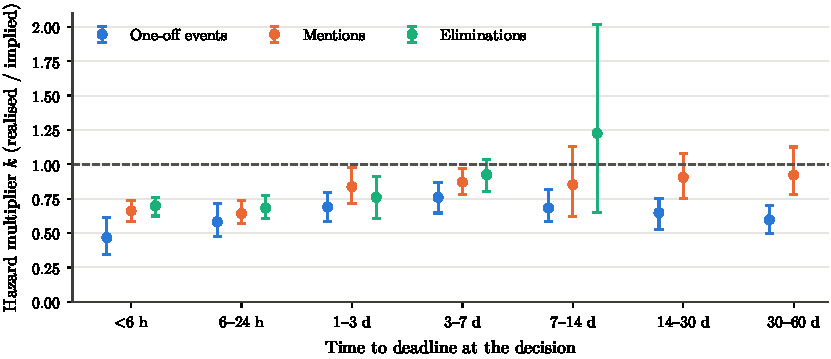
\includegraphics[width=\textwidth]{figures/fig_haz_calibration.pdf}
\caption{Hazard multiplier $k$ (realised over implied cumulative hazard) by lead and contract type,
all splits pooled, with 5th--95th percentile intervals from 200 cluster-bootstrap resamples. The
dashed line is perfect calibration. Cells with fewer than 30 observations are omitted.}
\label{haz-fig-calib}
% source: summary.json:calibration_by_kind_lead
\end{figure}

\subsubsection{Implied hazard term structures}\label{haz-res-term}

Across strips, the forward hazard curve is more often rising than flat. Of 3{,}019 daily snapshots
on 194 strips, 48\% are rising, 35\% front-loaded, 15\% flat and 2.4\% inverted, and the median ratio
of the last forward hazard to the spot hazard is 1.20 (\cref{haz-tab-term}).
% source: summary.json:term_structure_shapes
The shape differs by category in an interpretable way:
\begin{itemize}
\item Science and technology strips, mostly product-release dates, are rising in 61\% of snapshots
  with a median ratio of 2.0. The market expects a release later rather than sooner.
\item Climate strips (storm and seasonal milestones) are also rising.
\item Entertainment, sports and elections lean front-loaded (median ratios 0.70--0.89): if the
  occurrence does not come soon, it becomes less likely.
\item Politics is mixed, with a median ratio of 1.10.
\end{itemize}

Along a single contract, the implied hazard rises steeply as the deadline approaches without an event
(\cref{haz-fig-path-theta}a). Relative to its value seven days out, the median $\hbarimp$ is 1.4 times
higher at 72 hours, 2.3 times at 24 hours, 7 times at 6 hours and 33 times at one hour for politics.
Science and technology and entertainment follow nearly the same path; mentions are milder, at 10
times at one hour.
% source: summary.json:decay_paths_by_category (anchor 168 h)
A flat deterministic hazard would keep this ratio at one. Taken at face value, prices imply a hazard
concentrated near the deadline; the timing evidence below shows that realised hazards are concentrated
there too, but by much less.

\begin{table}[t]
\centering
\begin{threeparttable}
\caption{Hazard term-structure shapes and static-arbitrage frequency by category}\label{haz-tab-term}
\footnotesize
% source: summary.json:term_structure_shapes:by_category and summary.json:static_arbitrage_by_category
\setlength{\tabcolsep}{4pt}
\begin{tabular}{@{}lrrrrrrrrrr@{}}
\toprule
 & \multicolumn{6}{c}{Forward-hazard shape (daily snapshots)} & \multicolumn{4}{c}{Adjacent nested pairs (hourly)} \\
\cmidrule(lr){2-7}\cmidrule(l){8-11}
Category & Snap. & Strips & $h_{\mathrm{fwd}}/h_{\mathrm{spot}}$ & Rising & Front & Inv. & Pair-h & $p_1>p_2$ & Crossed & Exec. \\
\midrule
Politics          & 1{,}631 & 102 & 1.10 & 0.44 & 0.35 & 0.024 & 63{,}520 & 0.022 & 0.0016 & 0.0008 \\
Science \& tech.  &    783 &  38 & 2.02 & 0.61 & 0.29 & 0.022 & 32{,}955 & 0.033 & 0.0012 & 0.0007 \\
Entertainment     &    400 &  22 & 0.89 & 0.41 & 0.45 & 0.022 & 15{,}108 & 0.060 & 0.0017 & 0.0012 \\
Sports            &    126 &  17 & 0.70 & 0.43 & 0.48 & 0.048 & 14{,}173 & 0.044 & 0.0018 & 0.0011 \\
Elections         &     46 &   9 & 0.89 & 0.39 & 0.46 & 0.022 &  2{,}196 & 0.010 & 0.0005 & 0.0005 \\
Climate \& weather &    33 &   6 & 1.74 & 0.70 & 0.09 & 0.000 &  2{,}467 & 0.149 & 0.0004 & 0.0004 \\
\midrule
All               & 3{,}019 & 194 & 1.20 & 0.48 & 0.35 & 0.024 & 130{,}419 & 0.034 & & \\
\bottomrule
\end{tabular}
\begin{tablenotes}\footnotesize
\item Left: one snapshot per strip and day (16:00 UTC candle, spread at most 10\textcent), legs open,
windows started and nested. $h_{\mathrm{fwd}}/h_{\mathrm{spot}}$ is the median ratio of the last
forward hazard to the spot hazard to the first deadline. Rising: ratio above 1.25; Front: below 0.8;
Inv.: some forward hazard negative; the remaining share is flat. Right: adjacent nested legs quoted in
the same hourly candle. $p_1>p_2$: the earlier deadline's mid exceeds the later one's. Crossed: the
earlier bid exceeds the later ask. Exec.: the crossing survives the taker fee on both legs. Shares of
pair-hours; all splits pooled.
\end{tablenotes}
\end{threeparttable}
\end{table}

\subsubsection{Theta: prices decay too slowly near the deadline}\label{haz-res-theta}

Conditional on no event, prices fall more slowly than the flat-hazard theta at every lead
(\cref{haz-tab-theta}). The realised no-event change is 28--69\% of the model change, and the gap is
significant everywhere ($t$ between 3.6 and 11.5). Jumps are also rarer than the implied hazard
predicts: 18 against 74 expected in the last six hours, and 40 against 98 at 6--24 hours. The two
effects net out to a near-zero martingale drift at most leads. The exception is the last six hours,
where prices fall by 0.86\cents{} per grid step on average ($t=-7.2$), and marginally the 14--30 day
leads ($-1.3$\cents, $t=-2.1$).
% source: summary.json:theta (group core)
Read together, slow decay and rare jumps mean that the price path is close to a martingale away from
the deadline but not in the final hours. In those hours the excess is not removed by decay and is
paid off only at settlement.

\begin{table}[t]
\centering
\begin{threeparttable}
\caption{Theta, jumps and martingale drift over the next grid step (events, mentions and counts)}\label{haz-tab-theta}
\footnotesize
% source: data/research/pm_hazard/summary.json:theta (group = core)
\begin{tabular}{@{}lrrrrrrrr@{}}
\toprule
 & & & \multicolumn{2}{c}{Jumps} & \multicolumn{3}{c}{No-event change (\textcent)} & \\
\cmidrule(lr){4-5}\cmidrule(lr){6-8}
Lead & $n$ (cl.) & Drift \textcent{} ($t$) & Real. & Flat & Real. & Flat & Ratio ($t$ gap) & $\sigma_{\ln\hbarimp}$ \\
\midrule
$<6$ h   & 3{,}580 (451) & $-0.86$ ($-7.18$) &  18 &  74.2 & $-1.19$ & $-1.85$ & 0.65 (10.1) & 2.23 \\
6--24 h  & 3{,}108 (355) & $-0.35$ ($-1.55$) &  40 &  98.1 & $-1.14$ & $-2.40$ & 0.48 (10.2) & 1.22 \\
1--3 d   & 2{,}771 (317) & $0.34$ ($1.12$)   &  72 & 168.9 & $-1.23$ & $-4.43$ & 0.28 (11.5) & 0.79 \\
3--7 d   & 2{,}994 (321) & $-0.31$ ($-0.58$) & 243 & 341.3 & $-4.42$ & $-6.40$ & 0.69 (3.6)  & 0.53 \\
7--14 d  & 1{,}303 (240) & $-0.28$ ($-0.59$) &  27 &  82.2 & $-1.38$ & $-3.98$ & 0.35 (5.6)  & 0.39 \\
14--30 d & 1{,}188 (238) & $-1.30$ ($-2.10$) &  65 & 126.1 & $-3.76$ & $-6.00$ & 0.63 (4.5)  & 0.27 \\
30--60 d &    792 (189) & $-0.28$ ($-0.32$) &  70 & 106.0 & $-3.83$ & $-6.38$ & 0.60 (3.6)  & 0.21 \\
\bottomrule
\end{tabular}
\begin{tablenotes}\footnotesize
\item Priced observations (spread at most 10\textcent, mid below 0.9, no event yet), all splits pooled;
the step runs to the next grid point (to $T$ at the 1-hour lead). Drift: mean price change with the
price set to 1 after a jump, $t$ clustered by event. Jumps: realised count against the flat-hazard
expectation $\sum(1-e^{-\hbarimp\Delta})$. No-event change: mean realised mid change against the
flat-hazard theta $(1-p)(1-e^{\hbarimp\Delta})$. Ratio: realised over model, with the clustered $t$ of
their difference. $\sigma_{\ln\hbarimp}$: standard deviation of $\Delta\ln\hbarimp/\sqrt{\Delta}$ per
square-root day on no-jump steps. Conditioning on ``no event'' uses the event-time upper bound and is
descriptive.
\end{tablenotes}
\end{threeparttable}
\end{table}

\Cref{haz-fig-path-theta}b follows the 15--50\cents{} cohort from seven days out. With no event, the
mean price is still 41\% of its starting level 24 hours before the deadline (the flat model gives
16\%), 28\% at six hours (model 4\%) and 15\% one hour before (model 0.7\%). In levels this is
10.4\cents{} against 4.2\cents{} at 24 hours and 3.2\cents{} against 0.2\cents{} at one hour.
% source: summary.json:decay_paths (anchor 168, group core, p0_b 15-50)
Longshots starting below 15\cents{} (mean 5.6--6.2\cents) settle on a plateau of 1.4--2.1\cents{}
inside the last day, against model values of 0.03--0.9\cents. This plateau is largely the tick floor.
% source: summary.json:decay_paths (p0_b longshot<15)
Eliminations show the scheduled-event version of the same picture: no-event decay is only 12--31\%
of flat theta beyond six hours, because the price should not decay until the episode airs.
% source: summary.json:theta (group elimination)

\begin{figure}[t]
\centering
\begin{subfigure}[t]{0.49\textwidth}
\centering
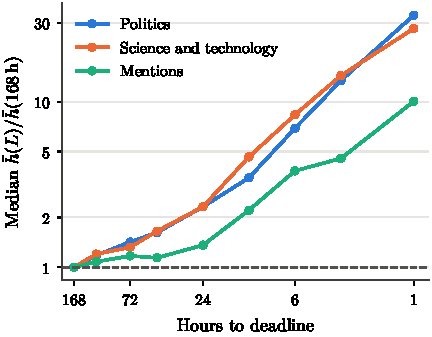
\includegraphics[width=\textwidth]{figures/fig_haz_hazard_path.pdf}
\caption{Median implied hazard relative to 168 h}
\end{subfigure}\hfill
\begin{subfigure}[t]{0.49\textwidth}
\centering
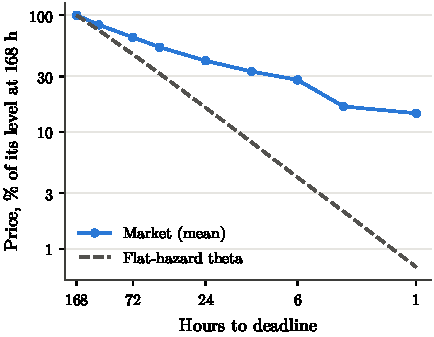
\includegraphics[width=\textwidth]{figures/fig_haz_theta.pdf}
\caption{Theta path, 15--50\textcent{} cohort}
\end{subfigure}
\caption{Implied hazard and price paths of deadline contracts with no event yet, anchored seven days
(168 h) before the deadline. (a)~Median of $\hbarimp(L)/\hbarimp(168\,\mathrm{h})$ for the three
largest categories; a flat deterministic hazard gives one (dashed). (b)~Mean price relative to its
anchor value for contracts priced 15--50\textcent{} at the anchor, against the flat-hazard theta path
$[1-(1-p_A)^{\tau_L/\tau_A}]/p_A$ (dashed). Both axes are logarithmic. Conditioning on no event uses
the event-time upper bound and is descriptive.}
\label{haz-fig-path-theta}
% source: summary.json:decay_paths_by_category; summary.json:decay_paths (core, 15-50, anchor 168)
\end{figure}

\subsubsection{When do deadline events happen?}\label{haz-res-timing}

Resolutions arrive later in the window than the flat implied hazard predicts
(\cref{haz-fig-timing-var}a). For the 807 event, mention and count contracts that resolved YES (238
clusters), the mean probability integral transform is 0.61 ($t=7.7$; Kolmogorov--Smirnov distance
0.16). Of these resolutions, 15.7\% fall in the last tenth of the window against 6.4\% under the flat
hazard, and 20\% in the final day.
% source: summary.json:event_timing:all_core
One-off events are the most back-loaded (mean PIT 0.65, $t=8.3$; 19.7\% in the last tenth). Mentions
follow at 0.60 ($t=4.6$), while counts are consistent with a flat hazard (0.52, $t=0.35$). Eliminations
are a scheduled reveal: their PIT is 0.95 and 84\% of resolutions fall in the last tenth.
% source: summary.json:event_timing:by_kind

This evidence and the calibration results fit together. Realised hazards do rise towards the
deadline, which is why a flat hazard misplaces events. But the market's implied hazard rises much
faster (\cref{haz-fig-path-theta}a). In the final six hours, the realised number of resolutions is a
quarter of what the prevailing implied hazards predict (18 against 74, \cref{haz-tab-theta}). The net
result is a deadline premium concentrated in the final day.

\begin{figure}[t]
\centering
\begin{subfigure}[t]{0.49\textwidth}
\centering
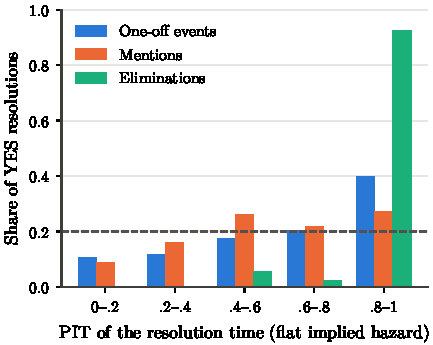
\includegraphics[width=\textwidth]{figures/fig_haz_timing.pdf}
\caption{Event timing}
\end{subfigure}\hfill
\begin{subfigure}[t]{0.49\textwidth}
\centering
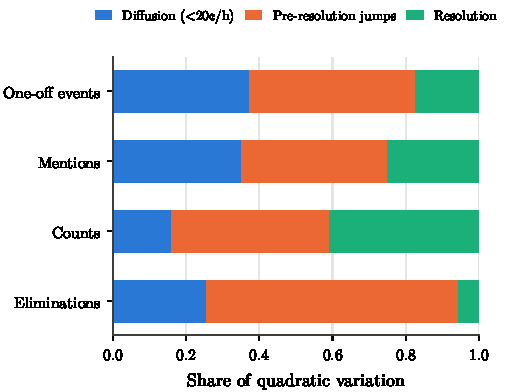
\includegraphics[width=\textwidth]{figures/fig_haz_variance.pdf}
\caption{Variance decomposition}
\end{subfigure}
\caption{(a)~Distribution of the probability integral transform of YES resolution times under the
flat hazard implied by the first priced pre-event quote; uniform (dashed) if the implied hazard shape
were right. (b)~Shares of the quadratic variation of the hourly mid up to settlement: diffusion
(hourly changes below 20\textcent), jumps of at least 20\textcent{} before resolution, and the
resolution step (the YES jump plus the NO deadline step).}
\label{haz-fig-timing-var}
% source: summary.json:event_timing:by_kind; summary.json:jump_diffusion_qv
\end{figure}

\subsubsection{Jumps, diffusion and the implied-hazard process}\label{haz-res-jumps}

Most price variance before resolution is news, not the resolution itself
(\cref{haz-fig-timing-var}b). For the 4{,}032 event, mention and count contracts with enough hourly
quotes, hourly changes below 20\cents{} account for 34\% of quadratic variation, and jumps of at
least 20\cents{} before resolution (about 0.5 per contract) for 42\%. The YES resolution jump accounts
for 23\%, and the NO deadline step for 0.8\%. Prices of contracts that resolve YES stand at 84\cents{}
on average two hours before the event-time bound, so the final jump averages 16\cents. The total is
1.19 times $\sum p_0(1-p_0)$, close to the martingale identity, with the excess consistent with
bid-ask bounce. Among events, mentions and counts, the YES resolution share is smallest for one-off events (16\%)
and largest for counts (37\%).
Eliminations are dominated by pre-resolution jumps (69\%), as episodes reveal information in large
steps.
% source: summary.json:jump_diffusion_qv

The implied hazard itself diffuses, with a volatility that rises towards the deadline. The standard
deviation of $\Delta\ln\hbarimp$ is 0.21--0.39 per square-root day beyond a week and 2.2 within six
hours (\cref{haz-tab-theta}). A CIR fit (\cref{haz-eq-cir}) is rejected as a description of
$\hbarimp$: the estimated mean reversion is negative at every horizon, $\kappa=-0.05$ per day beyond
three days and $-2.0$ within three days. The implied average hazard drifts upward towards the
deadline instead of reverting (\cref{haz-tab-cir}). A Cox model for these contracts therefore needs a
deterministic deadline-shaped component in the intensity, with diffusion around it of roughly 0.4 per
square-root day in log terms far from the deadline.
% source: summary.json:cir (group core)

\subsubsection{Static arbitrage across strips}\label{haz-res-arb}

Monotonicity violations are common at the mid but almost never executable (\cref{haz-tab-term}). Over
130{,}419 pair-hours on 898 adjacent nested pairs, the earlier deadline's mid exceeds the later one's
3.4\% of the time, but the earlier bid exceeds the later ask in only 0.04--0.18\% of pair-hours by
category. After taker fees, 108 pair-hours on 52 pairs in 36 strips remain, with a median locked-in
payoff of 0.8\cents{} per pair at unknown displayed size.
% source: summary.json:term_structure:monotonicity; summary.json:static_arbitrage_by_category
Calendar spreads show that forward segments are overpriced as well. In the \estim, the implied
conditional probability of an event between the two deadlines is 0.27 against a realised 0.21, and
buying the forward (NO on the near leg, YES on the far leg) loses 8.5\cents{} per pair ($t=-5.0$).
In the holdout it loses 7.2\cents{} ($t=-2.2$; 105 observations on 31 pairs).
% source: summary.json:term_structure:calendar

\subsubsection{Economic significance}\label{haz-res-econ}

The overpricing does not yield a robust trading rule (\cref{haz-tab-econ}). Buying NO when the
dev-fitted multiplier table shows an edge earns 19.0\cents{} per contract in-sample but $-5.3$\cents{}
($t=-0.8$; 49 trades in 13 clusters) in the holdout. A price-only calibration model does no better.
Buying NO on every quote below 50\cents{} earns 1.3\cents{} in the holdout ($t=1.65$), and 0.06\cents{}
on the first signal per contract. In a logistic blend with the mid, the hazard model's holdout
coefficient is 0.006 ($t=0.04$): out of sample it adds no information to the price.
% source: summary.json:economic

\subsubsection{Limitations}\label{haz-res-limits}
Several limitations qualify these results:
\begin{itemize}
\item The holdout is short: 2{,}076 priced observations, with at most 66 event clusters per lead cell.
% source: summary.json:universe:split_rows; summary.json:calibration_by_split
\item The event time is an upper bound. It makes resolutions look slightly late, biasing the timing
  PIT towards back-loading by an amount that is small relative to windows of days or weeks.
\item The one-cent tick floors longshot prices and explains much of their stickiness near the
  deadline.
\item History before 15 August 2026 comes from series chosen by title keyword. The choice does not
  depend on outcomes, but it can miss one-off series with other titles.
\item Strip nesting relies on the issuance order of legs.
\item The CIR fit uses an average rather than a spot intensity.
\end{itemize}


\section{Discussion}\label{sec:discussion}
\subsection{A unified description}

The three studies support one description of prediction-market prices. A binary contract's fair
price is a digital option on a latent state, written either as a score, as a numeric outcome, or as
the waiting time to an event. The state is revealed according to an information clock, with
short-lived random variation in the rate of revelation and a large share of discrete jumps:
\begin{align*}
  \text{single contract or ladder leg:}\quad &\pr_t=\Prob(Y_T>K\mid\F_t),\\
  &\dd Y_t=\alpha_t\,s(t)\,\dd W_t+J_t\,\dd N_t,\qquad \dd\alpha_t=\nu\alpha_t\,\dd B_t,\\
  \text{deadline contract:}\quad &\pr_t=1-\E_t\Big[e^{-\int_t^T h_u\dd u}\Big],\qquad
  h_u=h^{\det}(T-u)\,\xi_u ,
\end{align*}
where $h^{\det}$ is a deterministic hazard profile that rises into the deadline and $\xi$ a
log-diffusion. \Cref{tab:disc-facts} collects the estimates that pin down each component.

\begin{table}[t]
\centering
\begin{threeparttable}
\caption{Stylized facts by model component and contract type.}\label{tab:disc-facts}
\small
\begin{tabular}{@{}p{0.2\textwidth}p{0.36\textwidth}p{0.36\textwidth}@{}}
\toprule
Component & Estimate & Where it comes from \\
\midrule
Variance budget & realized variance over $\pr_0(1-\pr_0)$: 0.93--1.01 & weather, sports (\cref{sec:res-dyn}); 1.19 for deadlines (\cref{sec:res-haz}) \\
Clock & uniform in-game; back-loaded weather; flat pre-game; hazard rising into deadline & \cref{sec:res-dyn,sec:res-lad,sec:res-haz} \\
Backbone & $\beta\approx0.3$--$0.8$; logit-normal rejected & \cref{sec:res-dyn} \\
Stochastic volatility & half-life 7--21\,h (weather about 40\,h), $\nu\approx0.3$--$0.5$ per $\sqrt{\text{day}}$ & \cref{sec:res-dyn} \\
Jumps & 55--85\% of hourly variance; about half of in-game variance at 5--15\,s & \cref{sec:res-dyn,sec:res-hf} \\
Smile & convex, sticky in moneyness; tails too heavy & \cref{sec:res-lad} \\
Premia & implied tail mass, hazard and variance exceed realized & \cref{sec:res-lad,sec:res-haz} \\
\bottomrule
\end{tabular}
\end{threeparttable}
\end{table}

\subsection{Why clocks differ}

The information clock is the object that varies most across contract types, and it has a clear
economic reading: it is the schedule on which the world reveals the answer.
\begin{itemize}
  \item \emph{In-game sports.} Scoring opportunities arrive roughly uniformly in game time, so a
  uniform clock fits, exactly as in \citet{stern1994}.
  \item \emph{Pre-game sports.} Before the start almost nothing is learned, apart from occasional
  team news, so the clock runs at a few percent of the in-game rate.
  \item \emph{Weather.} Daily temperature extremes are revealed by observations late in the local
  day, giving a back-loaded clock with a pronounced time-of-day profile.
  \item \emph{Deadline contracts.} The implied hazard rises into the deadline. Part of this is real,
  since announcements do bunch late. But realized event timing is less concentrated than prices
  imply, so part of the rise is a premium (\cref{sec:res-haz}).
\end{itemize}

For pricing, the clock is to a binary contract what the term structure of implied variance is to
an option. A single contract's price carries no volatility information. A ladder's at-the-money
term structure and a deadline strip's forward hazards do, and both can be compared with the clock
measured from price paths.

\subsection{Jumps and the limits of the Gaussian model}

M0 gets the clock right and the shape wrong. Outside in-game sports, hourly standardised
innovations have excess kurtosis from tens to hundreds. Even within games, roughly half of
second-scale variance arrives in discrete moves. Several consequences follow.
\begin{itemize}
  \item \emph{Variance forecasts.} QLIKE and MSE rank the forecasting models differently: filtering
  the volatility state helps in quiet periods and hurts across jumps.
  \item \emph{Drift.} The outward drift of the probit price per unit of total variance falls short
  of the Gaussian prediction, as \cref{sec:model-m2} anticipates.
  \item \emph{Derivative pricing.} Any instrument that depends on the path, such as the
  variance and first-passage claims proposed by \citet{dalen2025}, must model jumps explicitly.
\end{itemize}

The basketball result is a useful benchmark. In the NBA, jump sizes scale with the Stern factor
$\varphi(\Zt)/\sqrt{\tauexp}$ almost exactly. In lower-scoring sports they scale less steeply.
This is consistent with scores that are rarer, larger and more state-dependent, for which
\citet{fengpolsonxu2016}'s Skellam model is the natural replacement.

\subsection{Backbone and smile dynamics}

The estimated backbone exponent of 0.3--0.8 places price volatility closer to the Wright--Fisher
(Jacobi) diffusion than to the logit-normal model that is common in practice. This independently
supports the Wright--Fisher component of \citet{xi2026}.

In ladders, the smile moves with the implied median: volatility at a fixed strike shifts as the
median moves, while at-the-money volatility does not slide along a fixed smile. In
\citet{derman1999}'s terms, the market treats the outcome distribution as a location--scale family
that is re-centred on news. That is natural when news shifts the expected outcome (a score, a
forecast update) without changing the remaining uncertainty much.

\subsection{A tail-and-time premium}

The one systematic departure from fair pricing appears in three forms:
\begin{itemize}
  \item implied tails across strikes are heavier than realized tails;
  \item implied hazards exceed realized hazards at every lead before a deadline, and prices decay
  more slowly than the hazard model requires;
  \item before and during games, ladders imply more variance than is subsequently realized.
\end{itemize}
In each case the market overprices the probability of an outcome far from the centre, or of an
event within a short window. This is the favourite--longshot bias of \citet{snowbergwolfers2010}
and \citet{burgi2025}, seen across strikes and across time.

Three features of the venue limit how far it can be corrected.
\begin{itemize}
  \item \emph{Tick grid.} The one-cent grid caps the gain from selling an overpriced 1--2\cents
  contract at about a cent.
  \item \emph{Fees.} Per-order rounding of fees makes small orders near the edges expensive.
  \item \emph{Collateral.} Selling a longshot requires posting nearly the full contract value as
  collateral.
\end{itemize}
In line with these limits, simple rules that sell the premium earn at most a few cents per contract
out of sample, and none is robust across samples. The premium is a stable feature of prices, not
an exploitable inefficiency at retail scale.

Two departures from the martingale property remain.
\begin{itemize}
  \item \emph{Weather.} Ladder medians for daily highs drift down overnight and up during the day.
  This may reflect a forecast input that under-predicts daytime maxima until observations arrive.
  \item \emph{Deadline contracts.} Prices fall faster than the martingale allows in their final
  hours, as stale prices catch up with the deadline.
\end{itemize}
Both are localised and small.

\subsection{Limitations}

The sample covers February to October 2026 for quotes and November 2026 for order books, a period
of rapid growth on the venue. Hourly candles hide intra-hour dynamics, and the base quote panel is
weighted toward actively traded markets. The order-book study covers two evenings and 50 game
markets.

We do not observe the game clock or the score. In-game time to expiry is measured to scheduled
settlement, which probably explains part of the cross-league dispersion. Event times of deadline
contracts are upper bounds inferred from prices and closing times.

Finally, we report many cells across categories, horizons and leads. We emphasise patterns that
hold in sign across the estimation and holdout samples, but individual cells should be read with
multiple testing in mind.


\section{Conclusion}\label{sec:conclusion}
We have proposed and calibrated an option-pricing framework for prediction-market contracts. A
binary contract is a digital option on a latent state, and its price dynamics are governed by an
information clock that releases a fixed variance budget $\pr_0(1-\pr_0)$. The Gaussian version
yields a Black--Scholes equation with a digital payoff and an exact transition law. A bounded SABR
extension and jumps bring it to the data. Strike ladders and deadline strips extend the framework
to implied distributions, smiles and hazard term structures.

On Kalshi:
\begin{itemize}
  \item the framework describes timing well, in that clocks are stable, category-specific and
  forecastable;
  \item it describes shape poorly unless jumps are included;
  \item it identifies a single pricing anomaly, a premium on tail outcomes and on short time
  windows.
\end{itemize}

Four extensions follow naturally:
\begin{itemize}
  \item using the game clock and score to test jump laws directly;
  \item longer order-book samples;
  \item contracts on the same outcome at two horizons, such as the first half and the full game,
  which would identify the clock without a model;
  \item pricing derivatives written on prediction-market prices, for which this framework supplies
  the dynamics.
\end{itemize}


\bibliographystyle{plainnat}
\bibliography{references,bib/dynamics,bib/ladders,bib/hazard}

\appendix
\section{Derivations}\label{app:derivations}
\paragraph{Proof of \cref{lem:variance}.}
Since $\pr$ is a square-integrable martingale, $\pr^2-\langle\pr\rangle$ is a martingale. Hence
$\E\langle\pr\rangle_T=\E\pr_T^2-\pr_0^2$. Because $\pr_T\in\{0,1\}$, $\pr_T^2=\pr_T$ and
$\E\pr_T=\pr_0$, so $\E\langle\pr\rangle_T=\pr_0-\pr_0^2$. For a discrete grid, martingale
increments are orthogonal, so
$\E\sum_i(\pr_{t_{i+1}}-\pr_{t_i})^2=\E(\pr_T-\pr_0)^2=\pr_0(1-\pr_0)$. \qed

\paragraph{Proof of \cref{prop:m0}.}
\emph{Price.} Given $\F_t$, $Y_T=Y_t+\int_t^T s\,\dd W\sim\N(Y_t,\Vrem_t)$, so
$\Prob(Y_T>0\mid\F_t)=\Phi(Y_t/\sqrt{\Vrem_t})$. Write $\pr(t,y)=\Phi(y/\sqrt{\Vrem_t})$. With
$\dot\Vrem_t=-s(t)^2$ and $\zeta=y/\sqrt{\Vrem_t}$:
\[
  \partial_t\pr=\varphi(\zeta)\,y\,\tfrac12\Vrem_t^{-3/2}s(t)^2,\qquad
  \partial_{yy}\pr=\varphi'(\zeta)/\Vrem_t=-\zeta\varphi(\zeta)/\Vrem_t .
\]
Hence $\partial_t\pr+\tfrac12 s^2\partial_{yy}\pr
=\tfrac12 s^2\varphi(\zeta)\big[y\Vrem^{-3/2}-\zeta\Vrem^{-1}\big]=0$. The terminal condition holds
because $\Vrem_t\to0$ as $t\to T$.

\emph{Dynamics.} By It\^o's formula for $\Zt=Y\Vrem^{-1/2}$,
\[
  \dd\Zt=\Vrem^{-1/2}s\,\dd W+Y\cdot\big(-\tfrac12\big)\Vrem^{-3/2}\dot\Vrem\,\dd t
  =\sqrt{\irate}\,\dd W+\tfrac12\irate\Zt\,\dd t .
\]
Applying It\^o to $\pr=\Phi(\Zt)$:
\[
  \dd\pr=\varphi(\Zt)\big(\sqrt{\irate}\,\dd W+\tfrac12\irate\Zt\,\dd t\big)+\tfrac12\varphi'(\Zt)\,\irate\,\dd t
  =\varphi(\Zt)\sqrt{\irate}\,\dd W ,
\]
since $\varphi'(z)=-z\varphi(z)$.

\emph{Transition.} $Y_{t+h}=Y_t+\xi$ with $\xi\sim\N(0,\Vrem_t-\Vrem_{t+h})$ independent of $\F_t$.
Then
\[
  \Zt_{t+h}=\frac{Y_t+\xi}{\sqrt{\Vrem_{t+h}}}=\Zt_t\sqrt{R}+\frac{\xi}{\sqrt{\Vrem_{t+h}}},
\]
and $\Var\big(\xi/\sqrt{\Vrem_{t+h}}\big)=(\Vrem_t-\Vrem_{t+h})/\Vrem_{t+h}=R-1$. The distribution of
$\pr_{t+h}$ follows because $\Phi$ is increasing. \qed

\paragraph{Uniform clock.} With $s$ constant, $\Vrem_t=s^2(T-t)$, $\irate_t=1/(T-t)$ and
$R=\tauexp/(\tauexp-h)$. For a power-law clock $\Vrem_t\propto\tauexp^{\gamma}$, $\irate_t=\gamma/\tauexp$.
A ladder whose at-the-money implied volatility scales as $\satm\propto\tauexp^{b}$ therefore implies
$\irate_t=2b/\tauexp$; Brownian information gives $b=\tfrac12$.

\paragraph{Backbone asymptotics.} Near zero, Mills' ratio gives
$\varphi(\Phi^{-1}(\pr))=\pr\,|\Phi^{-1}(\pr)|\,(1+o(1))$, and
$|\Phi^{-1}(\pr)|=\sqrt{2\ln(1/\pr)}\,(1+o(1))$. So
$\varphi(\Phi^{-1}(\pr))\sim\pr\sqrt{2\ln(1/\pr)}$, which lies between $g_1(\pr)\sim\pr$ and
$g_{1/2}(\pr)\sim\sqrt{\pr}$.

\paragraph{Proof of \cref{prop:smile}.}
(i) If $X_T\mid\F_t\sim\N(\Fmed,\sigma^2)$ then $S(K)=\Phi((\Fmed-K)/\sigma)$ and $\sigma_K=\sigma$ for
every $K$.

(ii) Let $X_T=\Fmed+\sigma_0\varepsilon$ with $\varepsilon$ symmetric, with distribution $G$ and
upper quartile $x_q$, so that $G(x_q)=\tfrac34$. Take $K>\Fmed$ and $x=(K-\Fmed)/\sigma_0$. Then
$S(K)=1-G(x)$ and $\sigma_K=\sigma_0\,x/\Phi^{-1}(G(x))$. Matching the interquartile range defines
$\satm=\sigma_0x_q/\Phi^{-1}(\tfrac34)$, so
\[
  \frac{\sigma_K}{\satm}=\frac{x}{x_q}\cdot\frac{\Phi^{-1}(\tfrac34)}{\Phi^{-1}(G(x))}.
\]
Heavier tails than the quartile-matched Gaussian means
$1-G(x)>1-\Phi\big(x\,\Phi^{-1}(\tfrac34)/x_q\big)$ for $x>x_q$. That is,
$\Phi^{-1}(G(x))<x\,\Phi^{-1}(\tfrac34)/x_q$, which gives $\sigma_K/\satm>1$. The case $K<\Fmed$
follows by symmetry. For a Student-$t$ with $\nu$ degrees of freedom, $x/\Phi^{-1}(G(x))$ is
increasing in $x>0$. We verified this numerically on a fine grid for $\nu\in[1.5,100]$; we do not
prove it in general. This gives monotonicity in $|m|$.

(iii) Under right skew the upper tail is heavier than the lower one, so by the same argument
applied to each tail separately, $\sigma_K$ is larger for $m>0$ than for $m<0$ at equal $|m|$.
\qed

\paragraph{Proof of \eqref{eq:varswap}.}
If $X_T\mid\F_t\sim\N(\Fmed_t,\satm(t)^2)$ for all $t$, then $\Fmed_t=\E[X_T\mid\F_t]$ is a martingale.
By the conditional-variance decomposition,
\[
  \satm(t)^2=\E_t\big[\satm(t+h)^2\big]+\Var_t(\Fmed_{t+h}) .
\]
Taking expectations gives \eqref{eq:varswap}. Without Gaussianity the identity holds for the
conditional mean and variance. The empirical version uses the median and the interquartile scale
as robust proxies. \qed

\paragraph{Proof of \cref{prop:hazard}.}
On $\{\vartheta>t\}$, $\Prob(\vartheta\le T\mid\F_t)=1-\E_t\exp(-\int_t^T h)$ is the standard
reduced-form survival formula \citep{lando1998}. For deterministic $h$,
$\pr_t=1-\exp(-H(t,T))$ with $\partial_tH=-h_t$, so $\dot\pr_t=-h_t e^{-H}=-h_t(1-\pr_t)$.

Write $D_t=\ind{\vartheta\le t}$. The price process is $\pr_t=D_t+(1-D_t)(1-e^{-H(t,T)})$, and
\[
  \dd\pr_t=(1-D_{t-})\big[-h_t(1-\pr_{t-})\,\dd t+(1-\pr_{t-})\,\dd D_t\big]
  =(1-D_{t-})(1-\pr_{t-})\big(\dd D_t-h_t\,\dd t\big).
\]
This is a martingale because $D_t-\int_0^{t\wedge\vartheta}h_u\,\dd u$ is one. For the term
structure, $1-\pr_t(T_i)=\exp(-H(t,T_i))$, so $H(T_1,T_2)=H(t,T_2)-H(t,T_1)\ge0$, and the forward
hazard formula follows. \qed

\section{Additional results: single-contract dynamics}\label{app:dyn}
% Additional results for the single-contract dynamics study.
% Sources: data/research/pm_vol/results_vi.json, results_cat.json (written by src/albert/research/pm_vol.py).

\paragraph{Variance identity.}
\Cref{tab:dyn-vi} reports the market-level check of the variance identity behind
\cref{sec:dyn-res-mart}.
The path share falls as the sampling interval grows,
  because two-sided quotes with spreads of at most 4\cents{} become sparse near resolution.
For sports the identity holds even though 93--95\% of the variance is realized after the
  last such quote, mostly in-game and at the final whistle.
Sampling every hour or every 24 hours gives the same picture.
  For weather the total ratio is 0.96, 0.97 and 0.96 on the estimation sample at 1, 6 and 24 hours.
  % source: results_vi.json:variance_identity (Climate and Weather, dev)

\begin{table}[ht]
\centering
\begin{threeparttable}
\caption{Variance identity by category}\label{tab:dyn-vi}
\scriptsize
\setlength{\tabcolsep}{3pt}
% source: data/research/pm_vol/results_vi.json:variance_identity (sample_h = 6)
\begin{tabular}{llrrcccc}
\toprule
Category & Split & Markets & Events & $\E(y-\pr_0)^2/\E\,\pr_0(1-\pr_0)$ ($t$) & Total ratio ($t$) & Path share & Terminal share \\
\midrule
Sports (all) & Est. & 9{,}533 & 8{,}551 & 0.99 ($-1.8$) & 0.98 ($-2.0$) & 0.07 & 0.93 \\
Sports (all) & Holdout & 10{,}007 & 8{,}991 & 1.01 (1.5) & 1.01 (1.3) & 0.05 & 0.95 \\
Weather & Est. & 5{,}838 & 1{,}183 & 0.96 ($-3.0$) & 0.97 ($-1.7$) & 0.29 & 0.70 \\
Weather & Holdout & 4{,}595 & 938 & 0.94 ($-3.2$) & 0.93 ($-3.1$) & 0.30 & 0.68 \\
Mentions & Est. & 336 & 109 & 1.05 (0.8) & 1.00 (0.0) & 0.27 & 0.73 \\
Mentions & Holdout & 478 & 98 & 1.20 (4.0) & 1.30 (4.7) & 0.23 & 0.82 \\
Politics & Est. & 274 & 102 & 1.34 (2.7) & 1.21 (1.9) & 0.68 & 0.44 \\
Politics & Holdout & 534 & 167 & 1.15 (1.5) & 1.26 (2.5) & 0.77 & 0.39 \\
Elections & Est. & 363 & 100 & 0.94 ($-0.8$) & 0.86 ($-1.6$) & 0.37 & 0.57 \\
Elections & Holdout & 369 & 120 & 1.30 (2.7) & 1.16 (1.6) & 0.72 & 0.38 \\
Entertainment & Est. & 438 & 174 & 1.24 (2.7) & 1.37 (3.5) & 0.84 & 0.39 \\
Entertainment & Holdout & 375 & 129 & 1.08 (0.8) & 1.06 (0.6) & 0.80 & 0.24 \\
Sci.\ \& Tech. & Est. & 333 & 96 & 1.19 (1.5) & 1.25 (1.9) & 0.85 & 0.32 \\
Sci.\ \& Tech. & Holdout & 382 & 129 & 1.53 (3.7) & 1.62 (3.9) & 1.25 & 0.23 \\
\bottomrule
\end{tabular}
\begin{tablenotes}[flushleft]\footnotesize
\item One row per market; quotes with spread $\le4$\cents{} sampled every 6 hours. $\pr_0$ is the first such mid and $y$ the settled outcome. \emph{Total ratio}: $\E[\sum(\Delta\pr)^2+(y-\pr_{\text{last}})^2]/\E[\pr_0(1-\pr_0)]$, which equals one for a calibrated martingale (\cref{sec:model}). \emph{Path} and \emph{terminal share}: the two parts of the numerator relative to it.
\item Split by close date: estimation sample (before 1 October 2026) and holdout (October 2026). This check fits no parameters, so Elections has a holdout here. $t$ for the mean difference from $\pr_0(1-\pr_0)$, clustered by event.
\item Candle samples outside sports and weather were partly selected on trading volume (ex post), which biases their ratios upward.
\end{tablenotes}
\end{threeparttable}
\end{table}

\paragraph{Backbone fits.}
\Cref{tab:dyn-backbone} gives the full backbone comparison behind \cref{sec:dyn-res-backbone} and
\cref{fig:dyn-backbone}.

\begin{table}[ht]
\centering
\begin{threeparttable}
\caption{Backbone estimates and QLIKE comparisons}\label{tab:dyn-backbone}
\scriptsize
\setlength{\tabcolsep}{2.2pt}
% source: data/research/pm_vol/results_cat.json:categories.*.backbone_table, beta_cells
\begin{tabular}{lccccccccc}
\toprule
 & \multicolumn{3}{c}{$\beta$} & \multicolumn{2}{c}{Est., vs.\ probit ($t$)} & \multicolumn{3}{c}{Holdout, vs.\ probit ($t$)} \\
\cmidrule(lr){2-4}\cmidrule(lr){5-6}\cmidrule(lr){7-9}
Category & QLIKE & Roll (s.e.) & Roll, hold. & Logit & Power & Logit & Power & Jacobi \\
\midrule
Sports in-game & 0.47 & 0.49 (0.14) & 0.35 & 0.016 (4.9) & $-0.020$ ($-1.8$) & 0.032 (4.7) & $-0.058$ ($-2.5$) & $-0.054$ ($-2.7$) \\
Sports pre-game & 0.39 & 0.44 (0.04) & 0.26 & 0.044 (6.2) & $-0.044$ ($-3.5$) & 0.070 (1.6) & $-0.090$ ($-1.6$) & $-0.075$ ($-1.7$) \\
Weather & 0.58 & 0.54 (0.04) & 0.69 & 0.054 (5.5) & $-0.029$ ($-2.7$) & 0.028 (2.8) & $-0.018$ ($-1.8$) & $-0.009$ ($-0.7$) \\
Mentions & 0.63 & 0.76 (0.11) & 0.60 & 0.045 (3.5) & $-0.014$ ($-1.1$) & 0.247 (1.2) & $-0.187$ ($-1.0$) & $-0.257$ ($-0.9$) \\
Politics & 0.39 & 0.49 (0.14) & 0.82 & 0.075 (4.0) & $-0.078$ ($-1.5$) & 0.161 (2.4) & $-0.144$ ($-1.2$) & $-0.142$ ($-1.4$) \\
Elections & 0.81 & 0.86 (0.10) & -- & 0.028 (1.0) & 0.000 ($-0.1$) & -- & -- & -- \\
Entertainment & 0.65 & 0.62 (0.05) & 0.95 & 0.040 (5.2) & $-0.014$ ($-1.9$) & $-0.005$ ($-0.2$) & 0.041 (1.6) & 0.108 (2.0) \\
Sci.\ \& Tech. & 0.31 & 0.51 (0.12) & 0.93 & 0.137 (7.8) & $-0.203$ ($-2.9$) & 0.081 (1.0) & $-0.572$ ($-1.2$) & $-0.595$ ($-1.3$) \\
\bottomrule
\end{tabular}
\begin{tablenotes}[flushleft]\footnotesize
\item Hourly steps; estimation sample (before 1 October 2026) and holdout (October 2026). \emph{QLIKE}: $\beta$ of the power backbone in \cref{eq:dyn-backbone}, fitted on the estimation sample. \emph{Roll}: log cell-mean regression on Roll-corrected $(\Delta\pr)^2$, with $\tauexp$-bucket fixed effects; standard errors from an event-level Poisson bootstrap (100 draws).
\item QLIKE differences are mean per-step losses relative to the probit backbone of M0 (negative: better than probit). Logit is $\beta=1$, Jacobi is $\beta=1/2$, and ``Power'' uses the estimated $\beta$. $t$ clustered by event.
\end{tablenotes}
\end{threeparttable}
\end{table}

\section{Additional results: strike ladders}\label{app:lad}
% Strike ladders: additional tables. Generated from data/research/pm_smile/summary.json.
This appendix reports the ladder sample by group (\cref{tab:lad-sample}), the smile parameters
for every group, lead and sample (\cref{tab:lad-smile-full}), the ATM term-structure exponents
(\cref{tab:lad-term}), the tail-mass comparison underlying \cref{fig:lad-calibration}
(\cref{tab:lad-tails}), the variance ratios underlying \cref{fig:lad-variance}
(\cref{tab:lad-variance}) and the economic-significance calculation (\cref{tab:lad-econ}).

\begin{table}[ht]
\centering\small
\begin{threeparttable}
\caption{Ladder sample by group.}\label{tab:lad-sample}
% source: data/research/pm_smile/summary.json:coverage
\begin{tabular}{@{}lrrrrrrr@{}}
\toprule
Group & Series & Events & Ladders & Snapshots & Leg quotes & Estimation & Holdout \\
\midrule
Weather highs & 24 & 1,531 & 1,531 & 5,762 & 34,572 & 3,286 & 2,476 \\
Weather lows & 24 & 836 & 836 & 1,509 & 9,054 & 801 & 708 \\
Sports totals & 149 & 3,778 & 3,778 & 7,762 & 78,874 & 4,245 & 3,517 \\
Team totals & 24 & 1,040 & 2,004 & 4,570 & 44,560 & 2,279 & 2,291 \\
Spreads & 44 & 1,760 & 1,760 & 4,010 & 61,022 & 1,740 & 2,270 \\
Politics & 11 & 115 & 115 & 270 & 2,157 & 110 & 160 \\
Entertainment & 11 & 82 & 82 & 207 & 1,775 & 122 & 85 \\
Science/tech & 14 & 33 & 33 & 57 & 280 & 34 & 23 \\
Other climate & 7 & 37 & 37 & 44 & 297 & 10 & 34 \\
Elections & 1 & 1 & 1 & 1 & 3 & 0 & 1 \\
\bottomrule
\end{tabular}
\begin{tablenotes}[flushleft]\footnotesize
\item Fitted snapshots (at least three survival points, median inside the quoted strikes). Leg
quotes: legs with spread at most 5\cents{} used in the fits. Estimation and holdout columns count
snapshots of events expiring before 1 October 2026 and in October 2026. Team-total events carry
one ladder per team.
\end{tablenotes}
\end{threeparttable}
\end{table}

\begin{table}[ht]
\centering\scriptsize
\setlength{\tabcolsep}{3.5pt}
\begin{threeparttable}
\caption{Smile parameters by group, lead and sample.}\label{tab:lad-smile-full}
% source: data/research/pm_smile/summary.json:smile (split dev = estimation, holdout)
\begin{tabular}{@{}llrrcccc@{}}
\toprule
Group & Lead & Snapshots & Strikes & $s$ [95\% CI] & $c$ [95\% CI] & Median $s$ & Median $c$ \\
\midrule
Weather highs & 36 h, est. & 668 & 1,758 & $-0.017$ [$-0.020$, $-0.013$] & 0.053 [0.051, 0.056] & $-0.024$ & 0.033 \\
Weather highs & 36 h, hold. & 489 & 1,162 & $-0.018$ [$-0.021$, $-0.014$] & 0.058 [0.056, 0.060] & $-0.025$ & 0.033 \\
Weather highs & 24 h, est. & 734 & 1,668 & $-0.019$ [$-0.022$, $-0.015$] & 0.054 [0.052, 0.056] & $-0.032$ & 0.035 \\
Weather highs & 24 h, hold. & 538 & 1,042 & $-0.015$ [$-0.018$, $-0.011$] & 0.056 [0.054, 0.059] & $-0.023$ & 0.033 \\
Weather highs & 16 h, est. & 741 & 1,348 & $-0.019$ [$-0.023$, $-0.016$] & 0.054 [0.051, 0.056] & $-0.036$ & 0.035 \\
Weather highs & 16 h, hold. & 553 & 876 & $-0.011$ [$-0.015$, $-0.008$] & 0.055 [0.052, 0.057] & $-0.019$ & 0.030 \\
Weather highs & 12 h, est. & 520 & 603 & 0.002 [$-0.003$, 0.006] & 0.058 [0.054, 0.062] & $-0.022$ & 0.030 \\
Weather highs & 12 h, hold. & 357 & 302 & $-0.004$ [$-0.011$, 0.003] & 0.053 [0.048, 0.058] & 0.004 & 0.033 \\
Weather lows & 36 h, est. & 87 & 205 & $-0.030$ [$-0.043$, $-0.018$] & 0.069 [0.061, 0.077] & $-0.041$ & 0.038 \\
Weather lows & 36 h, hold. & 15 & 33 & $-0.032$ [$-0.061$, $-0.003$] & 0.058 [0.046, 0.070] & $-0.014$ & 0.037 \\
Sports totals & 48 h, est. & 123 & 1,160 & 0.044 [0.037, 0.051] & 0.025 [0.018, 0.032] & 0.054 & 0.004 \\
Sports totals & 48 h, hold. & 175 & 1,498 & 0.057 [0.047, 0.068] & 0.038 [0.015, 0.061] & 0.059 & 0.005 \\
Sports totals & 24 h, est. & 986 & 7,702 & 0.068 [0.065, 0.072] & 0.021 [0.017, 0.024] & 0.086 & 0.001 \\
Sports totals & 24 h, hold. & 1,253 & 9,841 & 0.058 [0.056, 0.061] & 0.022 [0.018, 0.026] & 0.073 & 0.000 \\
Sports totals & 6 h, est. & 2,141 & 13,196 & 0.088 [0.085, 0.092] & 0.007 [0.005, 0.010] & 0.098 & $-0.007$ \\
Sports totals & 6 h, hold. & 1,574 & 12,494 & 0.057 [0.055, 0.059] & 0.018 [0.014, 0.021] & 0.071 & $-0.004$ \\
Sports totals & 1 h, est. & 995 & 4,954 & 0.117 [0.107, 0.127] & 0.026 [0.019, 0.033] & 0.155 & $-0.024$ \\
Sports totals & 1 h, hold. & 515 & 4,277 & 0.050 [0.044, 0.056] & 0.039 [0.036, 0.042] & 0.072 & 0.019 \\
Team totals & 48 h, est. & 103 & 806 & 0.000 [$-0.007$, 0.007] & 0.037 [0.033, 0.042] & 0.004 & 0.024 \\
Team totals & 48 h, hold. & 173 & 1,320 & 0.008 [0.004, 0.012] & 0.036 [0.033, 0.039] & 0.003 & 0.019 \\
Team totals & 24 h, est. & 730 & 4,246 & 0.052 [0.044, 0.059] & 0.043 [0.032, 0.053] & 0.075 & $-0.002$ \\
Team totals & 24 h, hold. & 851 & 6,758 & 0.035 [0.032, 0.039] & 0.022 [0.018, 0.025] & 0.038 & 0.002 \\
Team totals & 6 h, est. & 1,023 & 6,589 & 0.061 [0.056, 0.067] & 0.028 [0.024, 0.031] & 0.119 & $-0.011$ \\
Team totals & 6 h, hold. & 958 & 9,148 & 0.035 [0.031, 0.038] & 0.020 [0.016, 0.024] & 0.036 & $-0.006$ \\
Team totals & 1 h, est. & 423 & 1,555 & 0.114 [0.098, 0.131] & 0.041 [0.035, 0.048] & 0.202 & $-0.017$ \\
Team totals & 1 h, hold. & 309 & 2,247 & 0.028 [0.020, 0.035] & 0.050 [0.046, 0.054] & 0.038 & 0.026 \\
Spreads & 48 h, est. & 95 & 1,491 & 0.030 [0.014, 0.046] & 0.056 [0.049, 0.062] & $-0.001$ & 0.031 \\
Spreads & 48 h, hold. & 151 & 1,643 & 0.017 [$-0.004$, 0.037] & 0.055 [0.025, 0.085] & $-0.012$ & 0.025 \\
Spreads & 24 h, est. & 501 & 6,486 & 0.019 [0.013, 0.025] & 0.045 [0.040, 0.050] & 0.002 & 0.017 \\
Spreads & 24 h, hold. & 735 & 10,167 & 0.009 [0.003, 0.016] & 0.031 [0.023, 0.038] & $-0.002$ & 0.012 \\
Spreads & 6 h, est. & 755 & 7,711 & 0.017 [0.011, 0.023] & 0.053 [0.038, 0.068] & $-0.005$ & 0.008 \\
Spreads & 6 h, hold. & 966 & 12,318 & 0.006 [0.001, 0.012] & 0.036 [0.025, 0.047] & $-0.002$ & 0.010 \\
Spreads & 1 h, est. & 389 & 2,638 & 0.010 [$-0.001$, 0.021] & 0.062 [0.055, 0.068] & $-0.005$ & 0.030 \\
Spreads & 1 h, hold. & 418 & 4,467 & $-0.011$ [$-0.017$, $-0.006$] & 0.037 [0.034, 0.039] & $-0.016$ & 0.023 \\
Politics & 48 h, est. & 25 & 69 & 0.034 [$-0.002$, 0.070] & 0.057 [0.045, 0.069] & 0.078 & 0.044 \\
Politics & 48 h, hold. & 28 & 108 & 0.033 [0.011, 0.055] & 0.065 [0.052, 0.079] & 0.014 & 0.043 \\
Politics & 24 h, est. & 35 & 105 & $-0.001$ [$-0.022$, 0.021] & 0.083 [0.071, 0.095] & $-0.012$ & 0.071 \\
Politics & 24 h, hold. & 51 & 224 & 0.015 [$-0.004$, 0.034] & 0.068 [0.055, 0.081] & 0.007 & 0.052 \\
Politics & 6 h, est. & 32 & 76 & 0.002 [$-0.025$, 0.028] & 0.066 [0.055, 0.077] & 0.001 & 0.072 \\
Politics & 6 h, hold. & 51 & 177 & 0.010 [$-0.013$, 0.032] & 0.074 [0.064, 0.084] & 0.013 & 0.060 \\
Science/tech & 48 h, hold. & 14 & 34 & 0.012 [$-0.030$, 0.054] & 0.061 [0.037, 0.086] & 0.126 & 0.125 \\
Other climate & 24 h, hold. & 26 & 126 & 0.156 [0.135, 0.178] & 0.019 [0.003, 0.035] & 0.164 & 0.009 \\
\bottomrule
\end{tabular}
\begin{tablenotes}[flushleft]\footnotesize
\item Pooled least squares of $\sigma_K/\satm-1=a+s\,m+c\,m^2$ over off-ATM strikes ($|z|\ge0.25$,
$|m|\le3.5$, the two strikes straddling $\Fmed$ excluded) in cells with at least 30 strikes;
est.\ = estimation sample (before 1 October 2026), hold.\ = holdout (October 2026); 95\% intervals
from standard errors clustered by event. Median $s$, $c$: medians of the per-snapshot fits with
$a=0$ (snapshots with at least three off-ATM strikes).
\end{tablenotes}
\end{threeparttable}
\end{table}

\begin{table}[ht]
\centering\small
\begin{threeparttable}
\caption{ATM term structure: exponent of $\satm$ in the lead.}\label{tab:lad-term}
% source: data/research/pm_smile/summary.json:term_structure
\begin{tabular}{@{}lrrccc@{}}
\toprule
Group & Snapshots & Ladders & $\eta$ & 95\% CI & $t_{\eta=1/2}$ \\
\midrule
Weather highs & 5,640 & 1,409 & 0.773 & [0.760, 0.786] & 41.3 \\
Weather lows & 1,162 & 489 & 0.480 & [0.413, 0.546] & $-0.6$ \\
Sports totals & 4,749 & 2,227 & 0.009 & [0.007, 0.010] & $-595.8$ \\
Team totals & 3,430 & 1,580 & 0.001 & [$-0.003$, 0.005] & $-261.1$ \\
Spreads & 2,706 & 1,231 & 0.001 & [$-0.002$, 0.004] & $-325.9$ \\
Politics & 245 & 90 & 0.348 & [0.288, 0.408] & $-5.0$ \\
Entertainment & 184 & 59 & 0.186 & [0.138, 0.234] & $-12.7$ \\
Science/tech & 38 & 14 & 0.241 & [0.170, 0.311] & $-7.2$ \\
\bottomrule
\end{tabular}
\begin{tablenotes}[flushleft]\footnotesize
\item Within-ladder regression of $\log\satm$ on the log lead (ladders with at least two
snapshots), estimation sample and holdout pooled; intervals and $t$ clustered by event. Sports
use the pre-game leads (48, 24, 6 hours); weather leads are hours before the measurement-day close.
\end{tablenotes}
\end{threeparttable}
\end{table}

\begin{table}[ht]
\centering\scriptsize
\setlength{\tabcolsep}{3pt}
\begin{threeparttable}
\caption{Implied and realised tail mass beyond $|m|$ (cents per strike).}\label{tab:lad-tails}
% source: data/research/pm_smile/summary.json:tail_summary
\begin{tabular}{@{}llrccccrcccc@{}}
\toprule
 & & \multicolumn{5}{c}{Lower wing ($m\le-k$)} & \multicolumn{5}{c}{Upper wing ($m\ge k$)} \\
\cmidrule(lr){3-7}\cmidrule(lr){8-12}
Group & Sample, $k$ & Strikes & Implied & Realised & Normal & $z_{H_0}$ & Strikes & Implied & Realised & Normal & $z_{H_0}$ \\
\midrule
Weather highs & est., 1.5 & 5,031 & 2.17 & 0.97 & 1.07 & 0.83 & 5,545 & 1.85 & 0.63 & 1.12 & $-1.28$ \\
Weather highs & est., 2.5 & 2,953 & 1.11 & 0.30 & 0.09 & $-0.50$ & 3,386 & 0.95 & 0.03 & 0.09 & $-2.57$ \\
Weather highs & hold., 1.5 & 4,066 & 1.86 & 0.81 & 0.95 & 0.35 & 4,539 & 1.61 & 0.48 & 0.95 & $-1.74$ \\
Weather highs & hold., 2.5 & 2,580 & 1.05 & 0.00 & 0.09 & $-2.37$ & 2,959 & 0.93 & 0.00 & 0.07 & $-2.29$ \\
Weather lows & est., 1.5 & 2,221 & 2.14 & 0.54 & 0.95 & $-2.23$ & 1,425 & 0.96 & 0.00 & 0.58 & $-1.98$ \\
Weather lows & est., 2.5 & 1,552 & 1.54 & 0.32 & 0.01 & $-2.05$ & 949 & 0.65 & 0.00 & 0.14 & $-1.54$ \\
Weather lows & hold., 1.5 & 2,083 & 1.64 & 0.48 & 0.82 & $-1.49$ & 1,338 & 0.87 & 0.07 & 0.51 & $-1.49$ \\
Weather lows & hold., 2.5 & 1,471 & 1.14 & 0.14 & 0.01 & $-1.54$ & 925 & 0.66 & 0.00 & 0.15 & $-1.45$ \\
Sports totals & est., 1.5 & 936 & 3.45 & 2.35 & 4.05 & $-0.96$ & 2,200 & 5.90 & 6.18 & 3.35 & 0.67 \\
Sports totals & est., 2.5 & 157 & 0.66 & 0.64 & 0.24 & $-0.06$ & 456 & 1.77 & 2.19 & 0.18 & 0.45 \\
Sports totals & hold., 1.5 & 3,018 & 2.21 & 1.29 & 2.69 & $-0.71$ & 3,476 & 5.08 & 3.22 & 3.02 & $-0.77$ \\
Sports totals & hold., 2.5 & 858 & 0.55 & 0.00 & 0.12 & $-1.20$ & 914 & 1.70 & 0.11 & 0.15 & $-2.17$ \\
Team totals & est., 1.5 & 1,086 & 3.19 & 2.76 & 3.33 & $-0.30$ & 1,930 & 5.95 & 5.85 & 3.09 & 0.44 \\
Team totals & est., 2.5 & 158 & 0.80 & 0.00 & 0.20 & $-0.83$ & 362 & 3.62 & 1.10 & 0.19 & $-2.03$ \\
Team totals & hold., 1.5 & 1,933 & 3.35 & 2.85 & 3.24 & 0.34 & 2,551 & 4.51 & 4.74 & 2.96 & 1.46 \\
Team totals & hold., 2.5 & 334 & 1.05 & 0.00 & 0.18 & $-1.00$ & 568 & 2.06 & 0.70 & 0.17 & $-0.89$ \\
Spreads & est., 1.5 & 2,097 & 4.46 & 6.82 & 3.17 & 0.59 & 501 & 5.88 & 5.79 & 3.72 & 0.65 \\
Spreads & est., 2.5 & 539 & 1.60 & 2.78 & 0.14 & 1.10 & 90 & 1.26 & 1.11 & 0.17 & 0.39 \\
Spreads & hold., 1.5 & 4,000 & 3.65 & 2.83 & 2.86 & $-1.02$ & 1,425 & 4.30 & 4.35 & 3.44 & $-0.63$ \\
Spreads & hold., 2.5 & 1,135 & 1.04 & 0.26 & 0.14 & $-1.74$ & 193 & 1.63 & 0.00 & 0.24 & $-1.23$ \\
Politics & est., 1.5 & 197 & 3.09 & 2.03 & 1.26 & 0.10 & 320 & 2.96 & 2.50 & 0.87 & 1.29 \\
Politics & est., 2.5 & 123 & 1.86 & 0.00 & 0.07 & $-0.84$ & 232 & 2.05 & 1.29 & 0.04 & 0.22 \\
Politics & hold., 1.5 & 343 & 3.23 & 0.87 & 1.14 & $-0.32$ & 454 & 3.32 & 1.54 & 0.78 & $-0.06$ \\
Politics & hold., 2.5 & 222 & 2.21 & 0.90 & 0.07 & $-0.37$ & 338 & 2.38 & 0.00 & 0.05 & $-1.23$ \\
Entertainment & est., 1.5 & 343 & 1.14 & 0.87 & 0.57 & $-0.30$ & 478 & 1.20 & 0.21 & 0.47 & $-0.80$ \\
Entertainment & est., 2.5 & 280 & 0.76 & 0.71 & 0.08 & $-0.38$ & 402 & 0.94 & 0.00 & 0.05 & $-0.68$ \\
Entertainment & hold., 1.5 & 383 & 1.02 & 0.26 & 0.39 & 1.01 & 485 & 1.03 & 0.00 & 0.30 & $-0.68$ \\
Entertainment & hold., 2.5 & 331 & 0.76 & 0.00 & 0.04 & $-0.53$ & 433 & 0.84 & 0.00 & 0.03 & $-0.56$ \\
\bottomrule
\end{tabular}
\begin{tablenotes}[flushleft]\footnotesize
\item All strikes beyond the threshold, all leads; est.\ = estimation sample (before 1 October
2026), hold.\ = holdout (October 2026). Implied: $S(K)$ in the upper wing, $1-S(K)$ in the lower
wing; realised: the corresponding settled indicator; Normal: $\Phi(-|m|)$, the tail of a normal
with the ATM width. $z_{H_0}$: event means of realised minus implied over the variance implied
by the quotes (events independent), which remains valid when no tail event occurs.
\end{tablenotes}
\end{threeparttable}
\end{table}

\begin{table}[ht]
\centering\small
\begin{threeparttable}
\caption{Realised and implied variance between consecutive snapshots.}\label{tab:lad-variance}
% source: data/research/pm_smile/summary.json:variance_between
\begin{tabular}{@{}llrrccccc@{}}
\toprule
Group & Window & Pairs & Events & RV & IV & RV/IV & 90\% CI & Drift ($t$) \\
\midrule
Weather highs & 36$\to$24 & 1,034 & 1,034 & 0.1356 & 0.1324 & 1.024 & [0.867, 1.243] & 0.065 (5.8) \\
Weather highs & 24$\to$16 & 1,142 & 1,142 & 0.1259 & 0.1922 & 0.655 & [0.584, 0.731] & $-0.046$ ($-4.5$) \\
Weather highs & 16$\to$12 & 816 & 816 & 0.3329 & 0.3070 & 1.084 & [0.946, 1.221] & 0.060 (3.0) \\
Weather highs & 16$\to$8 & 339 & 339 & 0.8501 & 0.8345 & 1.019 & [0.901, 1.153] & 0.176 (3.6) \\
Weather highs & 12$\to$8 & 713 & 713 & 1.0595 & 0.6849 & 1.547 & [1.374, 1.738] & 0.106 (2.8) \\
Weather lows & 16$\to$12 & 236 & 236 & 0.0206 & 0.0709 & 0.291 & [0.248, 0.332] & 0.084 (11.0) \\
Weather lows & 12$\to$8 & 320 & 320 & 0.0208 & 0.0251 & 0.828 & [0.259, 1.890] & 0.036 (4.6) \\
Sports totals & 48$\to$24 & 296 & 296 & 0.0023 & 0.0053 & -- & -- & 0.003 (0.9) \\
Sports totals & 24$\to$6 & 2,225 & 2,225 & 0.0041 & 0.0177 & 0.233 & [0.189, 0.290] & 0.003 (2.0) \\
Sports totals & 6$\to$1 & 1,462 & 1,462 & 0.2797 & 0.3122 & 0.896 & [0.810, 0.982] & 0.022 (1.6) \\
Team totals & 48$\to$24 & 270 & 142 & 0.0012 & $-0.0202$ & -- & -- & $-0.002$ ($-0.8$) \\
Team totals & 24$\to$6 & 1,575 & 822 & 0.0033 & $-0.0329$ & -- & -- & $-0.001$ ($-0.6$) \\
Team totals & 6$\to$1 & 716 & 434 & 0.3507 & 0.5417 & 0.647 & [0.590, 0.701] & $-0.009$ ($-0.4$) \\
Spreads & 48$\to$24 & 244 & 244 & 0.0019 & $-0.0326$ & -- & -- & 0.003 (1.1) \\
Spreads & 24$\to$6 & 1,230 & 1,230 & 0.0040 & $-0.0088$ & -- & -- & 0.001 (0.5) \\
Spreads & 6$\to$1 & 773 & 773 & 0.4392 & 0.4786 & 0.918 & [0.835, 1.040] & 0.013 (0.6) \\
Politics & 48$\to$24 & 46 & 46 & 0.3432 & 0.0819 & 4.191 & [0.760, 23.987] & $-0.099$ ($-1.1$) \\
Politics & 24$\to$6 & 68 & 68 & 0.2657 & 0.2554 & 1.040 & [0.367, 3.623] & $-0.027$ ($-0.4$) \\
Politics & 6$\to$1 & 32 & 32 & 1.5147 & 0.6672 & 2.270 & [1.187, 4.407] & 0.576 (3.0) \\
\bottomrule
\end{tabular}
\begin{tablenotes}[flushleft]\footnotesize
\item Consecutive snapshots $t\to u$ of one ladder (window in hours before expiry; weather windows
with at least 100 pairs), estimation sample and holdout pooled. RV: mean of
$((\Fmed_u-\Fmed_t)/\sigma_t)^2$; IV: mean of $1-(\sigma_u/\sigma_t)^2$, with $\sigma=\satm$. RV/IV is
reported where IV exceeds 0.01; 90\% interval from 200 cluster-bootstrap replications over events.
Drift: mean of $(\Fmed_u-\Fmed_t)/\sigma_t$ with $t$ clustered by event. Sports windows from 6 to 1
hours are in play.
\end{tablenotes}
\end{threeparttable}
\end{table}


\begin{table}[ht]
\centering\small
\begin{threeparttable}
\caption{Economic significance: selling the tail side of ladder legs.}\label{tab:lad-econ}
% source: data/research/pm_smile/summary.json:pooled_rules (scope "all groups")
\begin{tabular}{@{}lrrrrrrr@{}}
\toprule
 & & \multicolumn{3}{c}{Estimation sample} & \multicolumn{3}{c}{Holdout} \\
\cmidrule(lr){3-5}\cmidrule(lr){6-8}
Rule & Tail price & Contracts & PnL & $t_{\text{risk}}$ & Contracts & PnL & $t_{\text{risk}}$ \\
\midrule
Every wing leg & 23.67 & 92,217 & $-2.30$ & $-2.90$ & 108,284 & $-1.75$ & $-2.11$ \\
Model, $|m|\ge1.5$ & 4.39 & 12,977 & $-0.78$ & $-1.63$ & 17,443 & $-0.22$ & $-0.46$ \\
Model, $|m|\ge2$ & 2.76 & 5,227 & 0.02 & 0.04 & 6,491 & 0.65 & 1.39 \\
Model, $|m|\ge2.5$ & 2.36 & 2,741 & 0.23 & 0.43 & 3,006 & 1.10 & 1.99 \\
Price, tail $\le2$\cents & 1.61 & 2,572 & 0.31 & 0.73 & 3,821 & 0.25 & 0.65 \\
Price, tail $\le3$\cents & 2.08 & 4,650 & 0.22 & 0.53 & 6,924 & $-0.04$ & $-0.09$ \\
Price, tail $\le5$\cents & 3.08 & 9,510 & $-0.47$ & $-1.12$ & 12,913 & $-0.21$ & $-0.49$ \\
Price, tail $\le10$\cents & 5.49 & 20,252 & $-1.26$ & $-2.56$ & 27,288 & $-0.91$ & $-1.81$ \\
Price $\le5$\cents{} and $|m|<2$ & 3.71 & 4,800 & $-1.22$ & $-2.37$ & 6,757 & $-0.85$ & $-1.65$ \\
Price $\le5$\cents{} and $|m|\ge2$ & 2.41 & 4,710 & 0.29 & 0.62 & 6,156 & 0.49 & 1.08 \\
\bottomrule
\end{tabular}
\begin{tablenotes}[flushleft]\footnotesize
\item Pre-specified rules pooled over all groups and leads, not tuned. Each qualifying leg at each
snapshot is one contract: the side opposite the tail is bought at the snapshot candle's ask (or
$1-$bid) with the Kalshi taker fee of its series and held to settlement. Tail price: mean mid of the
tail side (cents). PnL in cents per contract. $t_{\text{risk}}$: mean over its standard error under
settlement risk at the market price (per-contract s.d.\ $\sqrt{p(1-p)}$ summed within an event,
events independent). Estimation sample: before 1 October 2026; holdout: October 2026.
\end{tablenotes}
\end{threeparttable}
\end{table}

\section{Additional results: deadline contracts}\label{app:haz}
% Deadline contracts: additional tables. Every number is taken from
% data/research/pm_hazard/summary.json (keys noted next to each table).

\paragraph{Calibration by category and for longshots.}
\Cref{haz-tab-category} breaks the calibration of \cref{haz-tab-calib} down by category, and
\cref{haz-tab-longshot} reports the two cheapest price buckets by lead. Below 5\cents{} the hazard
multiplier is bounded below at 0.02 by construction when a cell has no YES outcomes, and the
one-cent tick bounds the mid from below, so those cells mainly describe the price floor.

\begin{table}[ht]
\centering
\begin{threeparttable}
\caption{Calibration of implied hazards by category (events, mentions and counts)}\label{haz-tab-category}
\footnotesize
% source: data/research/pm_hazard/summary.json:calibration_core_category
\begin{tabular}{@{}llrrcr@{}}
\toprule
Category & Lead & $n$ (cl.) & Mid & $k$ [90\% int.] & $\bar y-\bar p$ (\textcent; $t$) \\
\midrule
Politics           & $<1$ d  & 2{,}387 (274) & 0.108 & 0.50 [0.40, 0.62] & $-2.18$ ($-5.61$) \\
                   & 1--7 d  & 2{,}076 (206) & 0.200 & 0.64 [0.52, 0.84] & $-3.98$ ($-3.10$) \\
                   & $\ge7$ d & 2{,}021 (210) & 0.228 & 0.65 [0.54, 0.79] & $-5.39$ ($-4.33$) \\
Mentions           & $<1$ d  & 3{,}822 (70)  & 0.236 & 0.65 [0.58, 0.74] & $-1.74$ ($-5.39$) \\
                   & 1--7 d  & 4{,}181 (66)  & 0.353 & 0.86 [0.77, 0.95] & $-1.75$ ($-2.47$) \\
                   & $\ge7$ d & 1{,}048 (21)  & 0.411 & 0.89 [0.76, 1.05] & $-2.00$ ($-1.25$) \\
Science \& tech.   & $<1$ d  &    687 (51)  & 0.032 & 0.23 [0.12, 0.36] & $-2.16$ ($-6.14$) \\
                   & 1--7 d  &    399 (41)  & 0.138 & 0.55 [0.32, 0.82] & $-4.49$ ($-2.19$) \\
                   & $\ge7$ d &    587 (47)  & 0.233 & 0.59 [0.43, 0.84] & $-6.39$ ($-2.69$) \\
Sports             & $<1$ d  &    404 (37)  & 0.112 & 0.58 [0.45, 0.72] & $-1.58$ ($-3.49$) \\
                   & 1--7 d  &    266 (31)  & 0.271 & 0.82 [0.67, 1.25] & $-2.33$ ($-1.11$) \\
                   & $\ge7$ d &    242 (29)  & 0.323 & 1.02 [0.76, 1.79] & $0.33$ ($0.10$) \\
Entertainment      & $<1$ d  &    429 (66)  & 0.058 & 0.85 [0.35, 1.56] & $-0.39$ ($-0.37$) \\
                   & 1--7 d  &    273 (41)  & 0.214 & 0.64 [0.44, 1.06] & $-3.12$ ($-1.65$) \\
                   & $\ge7$ d &    411 (52)  & 0.295 & 0.38 [0.28, 0.57] & $-12.95$ ($-4.08$) \\
Elections          & $<1$ d  &    327 (31)  & 0.050 & 0.97 [0.47, 1.80] & $-0.08$ ($-0.07$) \\
                   & 1--7 d  &    190 (24)  & 0.150 & 1.15 [0.60, 2.27] & $1.35$ ($0.36$) \\
                   & $\ge7$ d &    229 (28)  & 0.217 & 0.81 [0.43, 1.56] & $-2.93$ ($-0.59$) \\
Climate \& weather & $<1$ d  &     37 (6)   & 0.140 & 0.85 [0.43, 1.56] & $-0.47$ ($-0.42$) \\
                   & 1--7 d  &     52 (8)   & 0.170 & 2.00 [0.35, 10.45] & $4.17$ ($0.51$) \\
                   & $\ge7$ d &     60 (10)  & 0.231 & 0.91 [0.36, 2.36] & $-1.44$ ($-0.16$) \\
\bottomrule
\end{tabular}
\begin{tablenotes}\footnotesize
\item As \cref{haz-tab-calib}, all splits pooled, eliminations excluded. Four categories with fewer
than four contracts (culture, health, social, world) are omitted.
\end{tablenotes}
\end{threeparttable}
\end{table}

\begin{table}[ht]
\centering
\begin{threeparttable}
\caption{Calibration of cheap contracts by lead (events, mentions and counts)}\label{haz-tab-longshot}
\footnotesize
% source: data/research/pm_hazard/summary.json:calibration_core_lead_price (price_b 0-5, 5-15)
\begin{tabular}{@{}lrrrcrrrc@{}}
\toprule
 & \multicolumn{4}{c}{Mid below 5\textcent} & \multicolumn{4}{c}{Mid 5--15\textcent} \\
\cmidrule(lr){2-5}\cmidrule(l){6-9}
Lead & $n$ (cl.) & Mid & YES & $k$ [90\% int.] & $n$ (cl.) & Mid & YES & $k$ [90\% int.] \\
\midrule
$<6$ h   & 3{,}388 (482) & 0.013 & 0.001 & 0.04 [0.02, 0.13] & 315 (108) & 0.078 & 0.051 & 0.64 [0.35, 1.01] \\
6--24 h  & 2{,}456 (353) & 0.018 & 0.002 & 0.11 [0.02, 0.20] & 600 (138) & 0.082 & 0.045 & 0.54 [0.33, 0.77] \\
1--3 d   & 1{,}565 (303) & 0.023 & 0.010 & 0.45 [0.27, 0.69] & 894 (179) & 0.084 & 0.049 & 0.58 [0.43, 0.74] \\
3--7 d   &    952 (269) & 0.023 & 0.011 & 0.45 [0.22, 0.71] & 869 (216) & 0.089 & 0.074 & 0.82 [0.61, 1.07] \\
7--14 d  &    571 (174) & 0.025 & 0.011 & 0.42 [0.21, 0.78] & 501 (163) & 0.086 & 0.052 & 0.59 [0.36, 0.84] \\
14--30 d &    314 (123) & 0.025 & 0.016 & 0.64 [0.19, 1.17] & 393 (160) & 0.089 & 0.041 & 0.44 [0.27, 0.64] \\
30--60 d &    230 (73)  & 0.028 & 0.000 & $\le 0.02$        & 246 (101) & 0.093 & 0.033 & 0.34 [0.14, 0.58] \\
\bottomrule
\end{tabular}
\begin{tablenotes}\footnotesize
\item As \cref{haz-tab-calib}, all splits pooled. YES is the share of observations whose contract
resolved YES. $k$ is reported as $\le 0.02$ when a cell has no YES outcome.
\end{tablenotes}
\end{threeparttable}
\end{table}

\paragraph{Event timing by type, category and starting price.}
\Cref{haz-tab-timing} extends the timing evidence of \cref{haz-res-timing}. Relative to the flat implied
hazard, the mean PIT exceeds 0.5 in every category with at least 15 resolutions and in every
starting-price bucket, and significantly so everywhere except elections ($t=1.79$). Sports and entertainment, where resolutions often hinge on scheduled games or
releases, are the most back-loaded.

\begin{table}[ht]
\centering
\begin{threeparttable}
\caption{Timing of YES resolutions relative to the flat implied hazard}\label{haz-tab-timing}
\footnotesize
% source: data/research/pm_hazard/summary.json:event_timing (all_core, by_kind, by_category, by_p0)
\setlength{\tabcolsep}{4pt}
\begin{tabular}{@{}lrrrrrrr@{}}
\toprule
 & $n$ (cl.) & $p_0$ & Anchor (h) & Mean PIT ($t$) & KS & Last 10\%: real./flat & Last day \\
\midrule
Events, mentions, counts & 807 (238) & 0.561 & 120 & 0.61 (7.72) & 0.16 & 0.157 / 0.064 & 0.201 \\
\addlinespace
One-off events  & 304 (151) & 0.560 & 504 & 0.65 (8.34)  & 0.22 & 0.197 / 0.063 & 0.207 \\
Mentions        & 447 (66)  & 0.566 & 120 & 0.60 (4.56)  & 0.16 & 0.132 / 0.064 & 0.201 \\
Counts          &  56 (21)  & 0.525 & 120 & 0.52 (0.35)  & 0.13 & 0.143 / 0.066 & 0.161 \\
Eliminations    &  92 (45)  & 0.510 & 120 & 0.95 (19.03) & 0.81 & 0.837 / 0.067 & 0.913 \\
\addlinespace
Politics        & 223 (102) & 0.559 & 504 & 0.60 (4.05)  & 0.14 & 0.152 / 0.063 & 0.157 \\
Science \& tech. &  44 (18) & 0.609 & 420 & 0.64 (2.46)  & 0.33 & 0.114 / 0.060 & 0.136 \\
Sports          &  39 (15)  & 0.517 & 504 & 0.74 (6.59)  & 0.38 & 0.359 / 0.067 & 0.385 \\
Elections       &  32 (18)  & 0.497 & 204 & 0.60 (1.79)  & 0.23 & 0.219 / 0.067 & 0.281 \\
Entertainment   &  15 (14)  & 0.583 & 1080 & 0.78 (6.52) & 0.44 & 0.267 / 0.063 & 0.267 \\
\addlinespace
$p_0<0.15$      &  42 (33)  & 0.089 & 120 & 0.64 (2.66)  & 0.24 & 0.238 / 0.096 & 0.238 \\
$0.15\le p_0<0.5$ & 246 (132) & 0.327 & 120 & 0.60 (4.57) & 0.16 & 0.175 / 0.083 & 0.228 \\
$0.5\le p_0<0.9$  & 519 (191) & 0.710 & 120 & 0.62 (7.07) & 0.17 & 0.143 / 0.052 & 0.185 \\
\bottomrule
\end{tabular}
\begin{tablenotes}\footnotesize
\item Contracts that resolved YES, anchored at their earliest priced pre-event grid quote with mid
below 0.9 ($p_0$: mean anchor price; Anchor: median anchor lead). PIT: $F(u)=[1-(1-p_0)^u]/p_0$ at
the elapsed window share $u$ of the event-time upper bound; uniform under the flat implied hazard.
$t$ tests mean PIT $=0.5$ with clustering by event. KS: Kolmogorov--Smirnov distance from uniform.
Last 10\%: share of resolutions in the last tenth of the window, realised and under the flat implied
hazard. Last day: share within 24 hours of the deadline. Category and price rows cover events,
mentions and counts. All splits pooled.
\end{tablenotes}
\end{threeparttable}
\end{table}

\paragraph{Variance decomposition and Cox intensity.}
\Cref{haz-tab-qv} gives the quadratic-variation shares behind \cref{haz-fig-timing-var}b, and
\cref{haz-tab-cir} the CIR fit of \cref{haz-eq-cir}. The negative mean-reversion estimates at both
horizons are the formal counterpart of the rising single-contract hazard paths in
\cref{haz-fig-path-theta}a.

\begin{table}[ht]
\centering
\begin{threeparttable}
\caption{Quadratic variation of the hourly mid up to settlement}\label{haz-tab-qv}
\footnotesize
% source: data/research/pm_hazard/summary.json:jump_diffusion_qv
\setlength{\tabcolsep}{4pt}
\begin{tabular}{@{}lrrrrrrrrr@{}}
\toprule
 & & & & \multicolumn{4}{c}{Share of quadratic variation} & & \\
\cmidrule(lr){5-8}
Type & Contracts & YES & Hours & Diff. & Jumps & YES res. & NO step & QV ratio & YES jump \\
\midrule
Events, mentions, counts & 4{,}032 & 0.405 & 133 & 0.344 & 0.423 & 0.225 & 0.008 & 1.19 & 0.162 \\
One-off events & 1{,}983 & 0.267 & 181 & 0.372 & 0.454 & 0.163 & 0.011 & 1.09 & 0.156 \\
Mentions       & 1{,}778 & 0.564 & 113 & 0.352 & 0.397 & 0.250 & 0.001 & 1.23 & 0.148 \\
Counts         &    271 & 0.373 & 117 & 0.160 & 0.433 & 0.374 & 0.033 & 1.50 & 0.326 \\
Eliminations   & 1{,}388 & 0.105 &  13 & 0.256 & 0.689 & 0.045 & 0.010 & 0.96 & 0.056 \\
\bottomrule
\end{tabular}
\begin{tablenotes}\footnotesize
\item Hourly mids with spread at most 10\textcent{} from the first quote in the last 62 days before the
deadline; contracts with at least six such hours. YES: share resolving YES. Hours: median count.
Diff.: hourly changes below 20\textcent{} before resolution. Jumps: hourly changes of at least
20\textcent{} before resolution. YES res.: $(1-m)^2$ from the last mid at least two hours before the
event-time upper bound. NO step: $m^2$ from the last mid before the deadline. QV ratio:
$\sum QV/\sum p_0(1-p_0)$, which is one in expectation for a martingale. YES jump: mean $1-m$ for
contracts that resolved YES. All splits pooled.
\end{tablenotes}
\end{threeparttable}
\end{table}

\begin{table}[ht]
\centering
\begin{threeparttable}
\caption{CIR-type fit of the implied average hazard on no-event steps}\label{haz-tab-cir}
\footnotesize
% source: data/research/pm_hazard/summary.json:cir
\begin{tabular}{@{}llrrrrrrr@{}}
\toprule
Type & Leads & Steps & Contracts & Median $\hbarimp$ (/d) & $\kappa$ (/d) & $\theta$ (/d) & $\sigma$ & $\sigma_{\ln\hbarimp}$ \\
\midrule
Events, mentions, counts & $\ge 3$ d & 5{,}034 & 1{,}987 & 0.023 & $-0.049$ & $-0.0002$ & 0.23 & 0.42 \\
                         & $<3$ d    & 3{,}729 & 1{,}279 & 0.113 & $-1.987$ & $0.0146$  & 8.16 & 1.45 \\
One-off events           & $\ge 3$ d & 2{,}660 &    924 & 0.014 & $-0.060$ & $0.0003$  & 0.27 & 0.41 \\
                         & $<3$ d    & 1{,}276 &    510 & 0.101 & $-2.219$ & $0.0108$  & 9.27 & 1.54 \\
Mentions                 & $\ge 3$ d & 2{,}105 &    910 & 0.037 & $-0.006$ & $-0.0443$ & 0.14 & 0.41 \\
                         & $<3$ d    & 2{,}090 &    659 & 0.105 & $-2.049$ & $0.0193$  & 7.92 & 1.34 \\
Counts                   & $\ge 3$ d &    269 &    153 & 0.048 & $-0.190$ & $0.0006$  & 0.37 & 0.57 \\
                         & $<3$ d    &    363 &    110 & 0.212 & $-1.396$ & $-0.0015$ & 4.40 & 1.57 \\
Eliminations             & $\ge 3$ d &    451 &    276 & 0.048 & $-0.306$ & $-0.0224$ & 0.92 & 0.67 \\
                         & $<3$ d    &    767 &    313 & 0.222 & $-2.810$ & $0.0161$  & 10.34 & 2.02 \\
\bottomrule
\end{tabular}
\begin{tablenotes}\footnotesize
\item Least-squares fit of \cref{haz-eq-cir} to $\lambda=\hbarimp$ (per day) over no-jump grid steps
with both mids in $(0.02, 0.98)$ and spread at most 10\textcent; $\sigma^2$ is the mean squared
residual per unit time. $\sigma_{\ln\hbarimp}$: standard deviation of $\Delta\ln\hbarimp/\sqrt{\Delta t}$
per square-root day. Negative $\kappa$ means no mean reversion: $\hbarimp$ drifts upward towards the
deadline, so $\theta$ is not a long-run level. All splits pooled.
\end{tablenotes}
\end{threeparttable}
\end{table}

\paragraph{Economic significance.}
\Cref{haz-tab-econ} reports the trading test summarised in \cref{haz-res-econ}. Thresholds are chosen
on the \estim{} by the highest mean profit with at least 30 trades, so the \estim{} columns are
in-sample.

\begin{table}[ht]
\centering
\begin{threeparttable}
\caption{Economic significance: buying NO at the NO ask, held to settlement}\label{haz-tab-econ}
\footnotesize
% source: data/research/pm_hazard/summary.json:economic
\setlength{\tabcolsep}{4pt}
\begin{tabular}{@{}llrrrr@{}}
\toprule
 & & \multicolumn{2}{c}{Estimation sample} & \multicolumn{2}{c}{Holdout} \\
 & & \multicolumn{2}{c}{(before 1 October 2026)} & \multicolumn{2}{c}{(October 2026)} \\
\cmidrule(lr){3-4}\cmidrule(l){5-6}
Rule & Unit & Trades (cl.) & \textcent{} ($t$) & Trades (cl.) & \textcent{} ($t$) \\
\midrule
Hazard model, edge $\ge 0.12$  & every signal  &    538 (143) & $19.02$ ($5.02$) &     49 (13) & $-5.30$ ($-0.83$) \\
                               & first per contract & 311 (143) & $16.15$ ($4.95$) &   29 (13) & $-8.53$ ($-1.26$) \\
Price-only model, edge $\ge 0.08$ & every signal &   444 (163) & $9.83$ ($2.77$)  &     27 (12) & $-7.43$ ($-0.78$) \\
                               & first per contract & 344 (163) & $8.20$ ($2.60$)  &   20 (12) & $-4.02$ ($-0.49$) \\
Control, YES mid $\le 0.50$    & every signal  & 18{,}949 (593) & $1.16$ ($4.35$) & 1{,}737 (89) & $1.32$ ($1.65$) \\
                               & first per contract & 3{,}561 (593) & $1.89$ ($3.44$) & 294 (89) & $0.06$ ($0.03$) \\
Maker NO bid, hazard model     & per fill      &     48 (12)  & $6.06$ ($0.68$)  &     29 (13) & $-3.17$ ($-0.46$) \\
Maker NO bid, mid              & per fill      &     32 (11)  & $6.56$ ($0.63$)  &     14 (9)  & $-10.29$ ($-1.02$) \\
\bottomrule
\end{tabular}
\begin{tablenotes}\footnotesize
\item Profit in cents (\textcent) per contract. One contract per signal at the NO ask ($1-$ YES bid) with the Kalshi taker fee
$0.07\,m\,P(1-P)$ rounded up to \$0.0001, held to settlement; quotes with spread at most
10\textcent. The hazard model is a multiplier table by type, lead and price fitted on the \estim; the
price-only model uses price buckets only; thresholds and the control's price cap are chosen on the
\estim. Maker rows rest a NO bid at $\lfloor 1-p-\text{margin}\rfloor$ until the next grid point and
count a fill only if a later trade prints through it (shared trade tape from 30 July 2026). $t$ is
clustered by event. In a logistic blend of the outcome on the logits of the mid and of the hazard
model, the hazard coefficient is 0.006 ($t=0.04$) in the holdout; holdout Brier scores are 0.0459
(mid) and 0.0472 (hazard model).
\end{tablenotes}
\end{threeparttable}
\end{table}


\end{document}
